%% ----------------------------------------------------------------
%% Thesis.tex -- MAIN FILE (the one that you compile with LaTeX)
%% ---------------------------------------------------------------- 

% Set up the document
\documentclass[a4paper, 12pt, twoside]{Thesis}  % Use the "Thesis" style, based on the ECS Thesis style by Steve Gunn
\graphicspath{Figures/}  % Location of the graphics files (set up for graphics to be in PDF format)
% Include any extra LaTeX packages required
\bibliographystyle{apalike}  % Use the "unsrtnat" BibTeX style for formatting the Bibliography
\usepackage[square, authoryear, comma, sort&compress]{natbib}  % Use the "Natbib" style for the references in the Bibliography
\usepackage{verbatim}  % Needed for the "comment" environment to make LaTeX comments
\usepackage{vector}  % Allows "\bvec{}" and "\buvec{}" for "blackboard" style bold vectors in maths
\hypersetup{urlcolor=cyan, colorlinks=true, linktocpage=true}  % Colours hyperlinks in blue, but this can be distracting if there are many links.

%%%%%% Start: Kelvin's Packages %%%%%% 
%\usepackage{apacite}
\usepackage{mathtools, amsmath, amssymb, amsthm, mathrsfs}
\usepackage{placeins}
\usepackage{wrapfig}
\usepackage[noabbrev]{cleveref}
\usepackage[usenames,dvipsnames]{xcolor}
\usepackage{CJKutf8}
\usepackage{bm}
\usepackage{graphicx}
\usepackage{psfrag}
\usepackage{epstopdf}
\usepackage{tikz}
\usepackage{smartdiagram}
\usepackage{upgreek}
\usepackage{stfloats}
\usepackage{dsfont}
\usepackage{wrapfig}
\usepackage{subfigure}

%\usepackage{caption}
%\usepackage{subcaption}
%\usepackage{subfigure}
%\usepackage{subfig}

%%% FLOW CHARTS
\usepackage{tikz}
\usetikzlibrary{shapes, arrows}
\usetikzlibrary{calc,arrows,decorations.pathmorphing,backgrounds,fit,positioning,shapes.symbols,chains}
\usetikzlibrary{decorations.pathreplacing}

%%%%%% End: Kelvin's Packages %%%%%% 

%%%%%% Start: Kelvin's Macro's %%%%%% 

\newtheoremstyle{indented}{3pt}{3pt}{\addtolength{\leftskip}{2.5em}}{}{\bfseries}{.}{.5em}{}
\theoremstyle{indented}

\newcommand{\matern}{Mat\'{e}rn }
\newcommand{\maternmath}{Mat\acute{e}rn }
\renewcommand{\vec}[1]{\boldsymbol{#1}}
\newcommand{\incite}[1]{\citeauthor{#1} [\citeyear{#1}]}
\newcommand{\numberthis}{\addtocounter{equation}{1}\tag{\theequation}}
\DeclareMathOperator*{\argmin}{arg\,min}
\DeclareMathOperator*{\argmax}{arg\,max}
%%%%%% End: Kelvin's Macro's %%%%%% 


\newdimen\testtemp
\newcommand{\ru}[1]{%
  \testtemp #1%
  \advance\testtemp .5pt%
  \divide\testtemp 2%
  \hbox to \testtemp{\leaders\hbox to 1mm{%
    \vrule height1mm depth0pt width.25pt\hfil}\hfil}%
  \hbox to 0pt{\hss\vrule height3mm depth0pt width.25pt\hss}%
  \hbox to \testtemp{\leaders\hbox to 1mm{%
    \hfil\vrule height1mm depth0pt width.25pt}\hfil}}

\def\textfraction{.1}
\fboxsep=-\fboxrule
\newcommand{\figbox}[1]{%
  \fbox{%
    \vbox to 1in{%
      \vfil
      \hbox to 2in{%
        \parbox{2in}{%
          \centering
          #1}}%
      \vfil
      \vbox to 0pt{%
        \vss
        \hbox to 2in{%
          \hfil
          \ru{1.1in}%
          \hfil}}}}}
          
%% ----------------------------------------------------------------
\begin{document}
\frontmatter      % Begin Roman style (i, ii, iii, iv...) page numbering
\title  {
\includegraphics[width=0.25\textwidth]{Figures/University-of-Sydney.png} \\ Informative Seafloor Exploration {\Large{for}} Benthic Habitat Mapping}
\authors  {\texorpdfstring
            {\href{mailto:yhsu9975@uni.sydney.edu.au}{Kelvin Y.S. Hsu}}
            {Kelvin Y.S. Hsu}
            }
\addresses  {\groupname\\\deptname\\\univname}  % Do not change this here, instead these must be set in the "Thesis.cls" file, please look through it instead
\date       {\today}
\subject    {}
\keywords   {}

\maketitle
%% ----------------------------------------------------------------

\setstretch{1.3}  % It is better to have smaller font and larger line spacing than the other way round

% Define the page headers using the FancyHdr package and set up for one-sided printing
\fancyhead{}  % Clears all page headers and footers
\rhead{\thepage}  % Sets the right side header to show the page number
\lhead{}  % Clears the left side page header

\pagestyle{fancy}  % Finally, use the "fancy" page style to implement the FancyHdr headers

%% ----------------------------------------------------------------
% Declaration Page required for the Thesis, your institution may give you a different text to place here
\Declaration{

\addtocontents{toc}{\vspace{0em}}  % Add a gap in the Contents, for aesthetics

I, Kelvin Y.S. Hsu, declare that this thesis titled, `Informative Seafloor Exploration for Benthic Habitat Mapping' and the work presented in it are my own. I confirm that:

\begin{itemize} 
\item[\tiny{$\blacksquare$}] This work was done wholly or mainly while in candidature for a research degree at this University.
 
\item[\tiny{$\blacksquare$}] Where any part of this thesis has previously been submitted for a degree or any other qualification at this University or any other institution, this has been clearly stated.
 
\item[\tiny{$\blacksquare$}] Where I have consulted the published work of others, this is always clearly attributed.
 
\item[\tiny{$\blacksquare$}] Where I have quoted from the work of others, the source is always given. With the exception of such quotations, this thesis is entirely my own work.
 
\item[\tiny{$\blacksquare$}] I have acknowledged all main sources of help.
 
\item[\tiny{$\blacksquare$}] Where the thesis is based on work done by myself jointly with others, I have made clear exactly what was done by others and what I have contributed myself.
\\
\end{itemize}
 
 
Signed:\\
\rule[1em]{25em}{0.5pt}  % This prints a line for the signature
 
Date:\\
\rule[1em]{25em}{0.5pt}  % This prints a line to write the date
}
\clearpage  % Declaration ended, now start a new page

%% ----------------------------------------------------------------
% The "Funny Quote Page"
\pagestyle{empty}  % No headers or footers for the following pages

\null\vfill
% Now comes the "Funny Quote", written in italics
\begin{CJK*}{UTF8}{bsmi}
\textit{``{\CJKfamily{bkai}三人行, 必有我師焉}''} \\
\textit{``Along a journey with three people, there is always one person I can learn from.''}
\begin{flushright}
	{\CJKfamily{bkai}孔子} \\
	Confucius
\end{flushright}
\end{CJK*}

%\textit{``Whatever the mind can conceive and believe, it can achieve.''}
%
%\begin{flushright}
%	 Napoleon Hill
%\end{flushright}

%\textit{``Whether you think you can, or you think you can't - you're right.''}
%
%\begin{flushright}
%	Henry Ford
%\end{flushright}

\vfill\vfill\vfill\vfill\vfill\vfill\null
\clearpage  % Funny Quote page ended, start a new page
%% ----------------------------------------------------------------

% The Abstract Page
\addtotoc{Abstract}  % Add the "Abstract" page entry to the Contents
\abstract{
\addtocontents{toc}{\vspace{0em}}  % Add a gap in the Contents, for aesthetics
	\begin{center}
	\textbf{Informative Seafloor Exploration for Benthic Habitat Mapping} \\
	\end{center}
	While seafloor bathymetry have been mapped extensively over the last few decades, geological and ecological observations of seafloor benthic zones only began recently. Unlike bathymetric mapping, data collection of benthic imagery requires \textit{in situ} exploration - a significantly slower and costly endeavour. An efficient exploration policy would therefore require solving the informative path planning problem. This thesis investigates a Gaussian process based informative exploration policy for benthic habitat mapping. Emphasis is placed on a mutual information measure as an acquisition criterion that is computationally feasible. A novel acquisition function, the linearised model differential entropy, is defined and derived which exhibit outstanding properties as compard to non-mutual information measures or Monte Carlo based mutual information measures. Along with the proposed receding horizon formulation for path planning, this work demonstrates the computational feasibility and performance of non-myopic acquisition under mutual linearised model differential entropy. Such a method is tested on collected benthic and bathymetric datasets from past AUV missions Scott Reef, Western Australia.
}

\clearpage  % Abstract ended, start a new page
%% ----------------------------------------------------------------

\setstretch{1.3}  % Reset the line-spacing to 1.3 for body text (if it has changed)

% The Acknowledgements page, for thanking everyone
\acknowledgements{
\addtocontents{toc}{\vspace{0em}}  % Add a gap in the Contents, for aesthetics
%
I am deeply grateful for the support from my supervisors Stefan Williams and Simon O'Callaghan. To Stef, thank you for being so down to earth and easy to talk to. You always manage to point me to the right direction just when I need it. To Simon, thank you for being so approachable to talk to. You always listen to what I have to say and reply with kind suggestions. Thank you for patiently thinking through problems and saying `hm, that's interesting alright' with me everytime I discover something strange or new. You made it easy for me to share my ideas and thoughts without fearing being in the wrong. In short, thank you both for your awesomeness.

I would also like to express my thanks to the people at NICTA, who made the working environment fun and enjoyable. This thesis would not be possible without their understanding and support. To Alistair, I admire your clear thinking and explanations. You always seem to understand what I am trying to ask even when I myself have trouble identifying my confusion. Many of the ideas developed in this thesis were inspired by our discussions. To Dan, thank you for your thoughtful advices and suggestions throughout the year. You were always quick to point out interesting things that I can look into. Thank you for stepping me through some of the difficult concepts in the beginning and even patiently helping me hunt those frustrating bugs when things were not working so well. To Lachlan, thank you for all the wise advices throughout the year. I still remember your detailed explanation about Bayesian inference and the almost philosophical note about logic and probability theory during the summer. That was very cool to listen to.

Finally, I would like to thank my friends and family for being the supportive bunch they always have been. From all the silly chats, stress inspired rants, mutual mocking, to the understanding support and encouragement, I would not have managed this much without you all. 




%
}
\clearpage  % End of the Acknowledgements
%% ----------------------------------------------------------------

\pagestyle{fancy}  %The page style headers have been "empty" all this time, now use the "fancy" headers as defined before to bring them back

%% ----------------------------------------------------------------
\lhead{\emph{Contents}}  % Set the left side page header to "Contents"
\tableofcontents  % Write out the Table of Contents

%% ----------------------------------------------------------------
\lhead{\emph{List of Figures}}  % Set the left side page header to "List if Figures"
\listoffigures  % Write out the List of Figures

%% ----------------------------------------------------------------
\lhead{\emph{List of Tables}}  % Set the left side page header to "List of Tables"
\listoftables  % Write out the List of Tables

%% ----------------------------------------------------------------
\setstretch{1.3}  % Set the line spacing to 1.3, this makes the following tables easier to read
\clearpage  % Start a new page
\lhead{\emph{Abbreviations}}  % Set the left side page header to "Abbreviations"
\listofsymbols{ll}  % Include a list of Abbreviations (a table of two columns)
{
% \textbf{Acronym} & \textbf{W}hat (it) \textbf{S}tands \textbf{F}or \\
		ACFR & Australian Centre of Field Robotics \\
		API & Application Programming Interface \\
		AUV & Autonomous Underwater Vehicle \\
		AVA & All Versus All \\
		\\
		BO & Bayesian Optimisation \\
		\\
		CDF & Cumulative Distribution Function \\
		\\
		EP & Expectation Propagation \\
		\\
		iid & independent and identically distributed \\
		\\
		GP & Gaussian Process \\ 
		GPBC & Gaussian Process Binary Classification/Classifier \\
		GPC & Gaussian Process Classification/Classifier \\
		GPLSC & Gaussian Process Least Squares Classification/Classifier \\
		GPMC & Gaussian Process Multi-Class Classification/Classifier \\
		GPR & Gaussian Process Regression \\
		\\
		LIDAR & Light Detection And Ranging \\
		LMDE & Linearised Model Differential Entropy \\
		LP & Laplace Approximation \\
		\\
		MCPIE & Monte Carlo Predictive Information Entropy \\
		MDE & Model Differential Entropy \\
		MDP & Markov Decision Processes \\
		\\
		NICTA & National ICT Australia \\
		\\
		OVA & One Versus All \\
		\\
		P1NN & Probabilistic One Nearest Neighbor \\
		PDF & Probability Distribution Function \\
		PIE & Predictive Information Entropy \\
		PLS & Probabilistic Least Squares \\
		POMDP & Partially Observable Markov Decision Processes \\
		PRM	& Probabilistic Road Map \\
		\\
		SBO & Sequential Bayesian Optimisation \\
		SE & Squared Exponential \\
		SONAR & Sound Navigation And Ranging \\
}

%%% ----------------------------------------------------------------
\clearpage  % Start a new page
\lhead{\emph{Notations}}  % Set the left side page header to "Notations"
\listofnotations{llcll}  % Include a list of Notations (a four column table)
{
	% Constant Name & Symbol & = & Constant Value (with units) \\
	Index Sets & $I_{n}$ & $:=$ & $\{1, 2, \dots, n\}$ & where $n \in \mathbb{N}$ \\
	Sequences & $\{a_{i}\}_{i \in I_{n}}$ & $:=$ & $\{a_{1}, a_{2}, \dots, a_{n}\}$ & \\
	Vector Shorthand & $\bvec{a} := \{a_{i}\}_{i \in I_{n}}$ & $\equiv$ & $[a_{1}, a_{2}, \dots, a_{n}]^{T} \in \mathbb{C}^{n}$ & if $a_{i} \in \mathbb{C} \quad \forall i \in I_{n}$ \\
	Matrix Shorthand & $A := \{\bvec{a}_{i}\}_{i \in I_{n}}$ & $\equiv$ & $[\bvec{a}_{1}, \bvec{a}_{2}, \dots, \bvec{a}_{n}]^{T} \in \mathbb{C}^{n \times p}$ & if $\bvec{a}_{i} \in \mathbb{C}^{p} \quad \forall i \in I_{n}$ \\
	Matrix as Sets & $\bvec{a} \in A$ & $\equiv$ & $\exists \; i \in I_{n}$ s.t. $\bvec{a}_{i} = \bvec{a}$ & where $A := \{\bvec{a}_{i}\}_{i \in I_{n}}$ \\
	Matrix Union & $A_{1} \cup A_{2}$ & $\equiv$ & $\big\{ \bvec{a} \big| \{\bvec{a} \in A_{1}\} \cup \{\bvec{a} \in A_{2}\} \big\}$ & $A_{1}$ Order Precedence \\
	Matrix Intersection & $A_{1} \cap A_{2}$ & $\equiv$ & $\big\{ \bvec{a} \big| \{\bvec{a} \in A_{1}\} \cap \{\bvec{a} \in A_{2}\} \big\}$ & $A_{1}$ Order Precedence \\
	Matrix Exclusion & $A_{1} \backslash A_{2}$ & $\equiv$ & $\big\{ \bvec{a} \big| \{\bvec{a} \in A_{1}\} \cup \{\bvec{a} \notin A_{2}\} \big\}$ & $A_{1}$ Order Precedence \\
}

%%% ----------------------------------------------------------------
\clearpage  %Start a new page
\lhead{\emph{Nomenclature}}  % Set the left side page header to "Nomenclature"
\listofnomenclature{ll}  % Include a list of Nomenclature (a three column table)
{
	% symbol & name \\
	$\bvec{p}$ & Position Vector \\
	$\bvec{x}$ & Feature Vector \\
	$\bvec{x}'$ & Feature Vector \\
	$f$ & Latent Function \\
	$y$ & Target Output \\
	$m$ & Expectance/Mean Function \\
	$k$ & Kernel/Covariance Function \\
	$\Sigma$ & Covariance Matrix \textit{or} Length Scale Matrix \\
	$l_{ij}$ & Joint Length Scale of Axis $i$ and $j$ \\
	$\sigma_{f}$ & Kernel Sensitivity \\
	$\vec{\uptheta}$ & Hyperparameters \\
	$K$ & Data Kernel \textit{or} Training Kernel \\
	$K^{\star}$ & Inference Kernel \\
	$K^{\star \star}$ & Query Kernel \\
	$p$ & Number of Features \\
	$n$ & Number of Training Points \\
	$n^{\star}$ & Number of Query Points \\
	$n_{C}$ & Number of Classes \\
	$n_{S}$ & Number of Samples \\
	$\mathcal{P}$ & Spatial Space \\
	$\mathcal{X}$ & Feature Space \\
	$\mathcal{Y}$ & Target Space \\
	$\mathscr{P}$ & Spatial Space $\sigma$-algebra \\
	$\mathscr{X}$ & Feature Space $\sigma$-algebra \\
	$\mathscr{Y}$ & Target Space $\sigma$-algebra \\
	$P$ & Training Positions \\
	$X$ & Training Features \\
	$\bvec{y}$ & Training Target Outputs \\
	$\bvec{f}$ & Training Latents \\
	$P^{\star}$ & Query Positions \\
	$X^{\star}$ & Query Features \\
	$\bvec{y}^{\star}$ & Query Target Outputs  \\
	$\bvec{f}^{\star}$ & Query Latents \\
	$H$ & Entropy \textit{or} Model Representative Event \\
	$D$ & Data Observation Event \\
	$I$ & Information Criterion \textit{or} Acquisition Criterion \\
	$\mathcal{H}$ & Inference Model \\
	$\mathcal{D}$ & Data Set \\
	$\mathcal{N}$ & Gaussian Distribution \\
	$\mathcal{GP}$ & Gaussian Process \\
	$z$ & Bathymetric Depth \textit{or} Generic Dummy Variable \\
	$a_{s}$ & Aspect (Short Scale) \\
	$a_{l}$ & Aspect (Long Scale) \\
	$r_{s}$ & Rugosity (Short Scale) \\
	$r_{l}$ & Rugosity (Long Scale) \\
	$\sigma$ & Likelihood Response Function \textit{or} Sigmoid \textit{or} Softmax \\
	$\vec{\uppi}$ & Predictive Probabilities \\
	$\bar{\vec{\uppi}}$ & Expected Predictive Probabilities \\
	$W$ & Negative Log Likelihood Response Hessian \\
	$\tilde{\bvec{p}}^{\star}$ & Essential Empirical Joint Probability Distribution at Query Points \\
	$\mathds{1}$ & Indicator Function \\
	$\mathbb{F}$ & Probability Pre-Fusion  \textit{or} Frequency Counter Function \\
	$\mathbb{H}$ & Modified Heaviside Function \\
	$\bvec{\mathds{H}}$ & Vectorised Modified Heaviside Function \\
	$\mathbb{M}$ & Class Prediction Function \\
	$\bvec{\mathds{M}}$ & Vectorised Class Prediction Function \\
	$\bvec{\psi}$ & Relative Angle Coordinates \\
	$\bvec{\phi}$ & Absolute Angle Coordinates \\
	$T$ & Cumulative Sum \\
	$q_{p}$ & Path Generation Function \\
	$f_{e}$ & Feature Extraction \\
%	& \\ % Gap to separate the Roman symbols from the Greek
%	& \\ % Gap to separate the Roman symbols from the Greek

}
%%% ----------------------------------------------------------------
%% End of the pre-able, contents and lists of things
%% Begin the Dedication page


\lhead{Informative Seafloor Exploration for Benthic Habitat Mapping}
\setstretch{1.3}  % Return the line spacing back to 1.3

%\pagestyle{empty}  % Page style needs to be empty for this page
%\dedicatory{For/Dedicated to/To my\ldots}

\addtocontents{toc}{\vspace{2em}}  % Add a gap in the Contents, for aesthetics


%% ----------------------------------------------------------------
\mainmatter	  % Begin normal, numeric (1,2,3...) page numbering
\pagestyle{fancy}  % Return the page headers back to the "fancy" style

% Include the chapters of the thesis, as separate files
% Just uncomment the lines as you write the chapters

\chapter{Introduction}
\lhead{Introduction}
\label{Introduction}

	\section{Motivation}
	\label{Introduction:Motivation}
	
		Thanks to optical and acoustic depth sounding technology, detailed ocean terrain maps across a majority of the globe have become increasingly accessible. These information generally takes the form of \textit{Bathymetric} data - recordings of measured depth, slope, roughness, and similar structural information that summarises the seafloor topography. Currently, bathymetric data has been recorded with advanced techniques such as SONAR (\textbf{SO}und \textbf{N}avigation \textbf{A}nd \textbf{R}anging), LIDAR (\textbf{LI}ght \textbf{D}etection \textbf{A}nd \textbf{R}anging), and Multibeam Echosounder for more than half a century \citep{Niedzielski2013231, Colbo201441}. With such volume of bathymetric information, we can reconstruct accurate 3D models for the seafloor terrain through spatial analytics and modeling techniques \citep{Niedzielski2013231}.
		
		However, bathymetric data only contains information regarding the spatial structure of the marine terrain. It provides no indication towards the types of marine habitats that resides within parts of the ocean, nor does it contain clues regarding the minerals or natural resources that may be present. Today, less than five percent of seafloor habitats have been explored \citep{NOAA}. As the ocean covers more than 70\% of the globe, this leaves more than 67\% of the planet's habitats unexplored despite our deep reliance on much of these undiscovered ecosystems. With big data analysis becoming more feasible in recent years, there has been an increase in scientific and economical demands - from ecologist and geologists to resource and mining industries - for the ability to predict or infer the types of marine habitats or natural resources residing at various marine environments.
		
		Thus, unlike the case for bathymetric data, there is currently a lack of \textit{label} data, which is a summary of the habitats, resources, and other interesting properties observed at various parts of the ocean. This implies the need to map the ocean floor again for label data using vision based sensing equipments. In order to understand the ecological, geological, chemical, and archaeological aspects of the ocean floor, autonomous underwater vehicles (AUVs) are now capable of efficiently collecting information and observations from natural environments of large spatial scale. In the case of benthic habitat mapping, AUVs collect imagery data of seafloor environments, which are then associated with a particular \textit{label} with semantic meaning \citep{Steinberg2015128}. For example, imageries of `coral' regions receive the label `coral'. Unfortunately, while bathymetric data can often be measured with decent accuracy at a distance (for example, with SONAR from ships at sea level), such visual imagery can only be obtained through expensive AUV missions that travel deep into the ocean to image underwater environments at a close distance. Together with the immense spatial scale of the benthic seafloor to be explored, this implies that it is impractical to map exhaustively the entire region of interest (ROI) under any reasonable time and cost. Furthermore, AUV missions are limited by power supply, data storage, and computational capabilities \citep{AsherBender}, further limiting the time and hence coverage each AUV mission can achieve. 
		
		As such, AUVs must prioritise exploring sub-domains of the ROI that ideally contain the most important and valuable information. This is a form of spatial sampling problem \citep{Rigby:ROB20372}, which aims to address the question: given the choice to observe only a few parts of the region of interest, how should one infer the best candidates for observation? AUV missions add another layer of complication to the spatial sampling problem - the candidate locations must form continuous paths that the AUV can physically travel.
		
		This is known as the \textit{informative path planning problem}. The objective of informative path planning is to minimise the overall uncertainty regarding the entire region of interest by traversing the most informative path.
		
		This thesis addresses the informative path planning problem for benthic habitat mapping. There are two main aspects to informative seafloor exploration for which this thesis is concerned with. The first part of this thesis is focused on benthic habitat mapping, where techniques of habitat classification and inference are discussed. The basic theory under which information and uncertainty are measured and quantified are developed and formulated in the general framework, which is then applied to benthic habitat mapping. The second part of this thesis then proceeds to investigate the informative seafloor exploration problem. Using the properties of inference models developed for benthic habitat mapping, a range of path planning policies are discussed and compared. Practical considerations of computational tractability and flexibility then lead to compromises between optimality and feasibility. Finally, this thesis proposes a practical framework for AUVs to autonomously plan informative paths that achieves the highest mapping rate under a classification accuracy criterion.
		
	\section{Objectives}
	\label{Introduction:Objective}
		The high level objective of this thesis is to develop an informative seafloor exploration policy that can produce benthic habitat maps efficiently. Specifically, this thesis focuses on the theoretical and computational aspects of informative path planning that is practical for seafloor mapping. The aim is to address the informative seafloor exploration problem in a principled manner with theoretical grounding, while taking computational feasibility into account. 
		
		The goal of this thesis can be summarised as follows:
		
		\begin{quote}
			To investigate informative seafloor exploration policies for an AUV with limited mission time, in order to map benthic habitats faster in a principled and computationally feasible way.
		\end{quote}
%	
%		The high level objective of this thesis is to develop and design an underwater path planner such that the resulting path minimises the overall mapping error of the seafloor region of interest.
%		
%		Detailed examination of this objective would raise details that would need to be made more specific.
%		
%		Firstly, the measure of entropy would be highly dependent on the quantities or qualities the vehicle is to search for, as well as the underwater region of interest. It would need to be examined to ensure that it is an appropriate measure of the environment uncertainty to be reduced that is relevant to the mission.
%		
%		Secondly, finding paths that subsequently minimises the overall entropy is fundamentally a dynamic programming and optimisation problem. As with any optimisation problem, problem constraints are to be defined and made clear. Within the presence of possibly difficult dynamical constraints, it is likely that simplifications are necessary at various stages of the thesis.
%		
%		Another consideration is the feasibility of the algorithm. While it can be difficult to measure the optimality of any solution proposed, it is often easier to examine the feasibility of the algorithm through studying the hardware constraints involved or the physical environment. One of the most important feasibility constraint relevant to this thesis is the computational capabilities of the vehicle computer hardware. Depending on the final proposed algorithm, it may not always be possible for the path planer to be executed in a fully online fashion. A more likely situation would involve planning a path to be executed for a duration of time and update the path through re-planning at a frequency much lower than the vehicle is navigating. For short missions, it may be more desirable to have the entire path planned offline.
%		
%		Other subtleties arise from the nature of the the underwater path planning problem. There is often no goal location, only an objective to maximise the information gained. This is a form of active path planning, which is similar to the active sampling philosophy but with dynamic constraints.
%		
%		Finally, other than the path planning algorithm, a major part of this thesis revolves around modeling the ocean environment accurately. Without an accurate understanding of the ocean environment, the vehicle cannot plan a path that is of reasonable significance. This thesis is to address the ways the ocean environment is to be modeled, develop these algorithms, and implement them on an ocean exploration setting.
%		
%		The detailed objective of this thesis is thus to examine and address all the concerns above, and to provide a better understanding towards the methods these active path planning problems can be approached.
		
	\section{Contribution}
	\label{Introduction:Contribution}
	
		This thesis is concerned with mapping seafloor benthic habitats efficiently in a principled manner. Specific contributions and focuses of this thesis are:
		
		\begin{itemize}
		
			\item A computationally efficient, parallelisable implementation for multiclass Gaussian process (GP) classifiers through the One versus All (OVA) scheme. Time and spatial complexity of the classifier are further improved through taking advantage of the GP classifier structure. Under Laplace approximation, this approach avoids the computational complexity from Monte Carlo sampling that is required in the inference stage. The computational framework is consistent with sparsification techniques for further complexity improvement although this is not necessary.
			
			\item An All versus All (AVA) approach to GP multiclass classification. While OVA techniques have been employed in various settings in the literature, there is no direct treatment of GP multiclass classification using All versus All classifiers, which achieves predictions with less biases due to a more balanced binary comparison between classes \textit{under balanced data}. It also shares the above advantages with OVA classifiers. This provides another choice for GP multiclass classification apart from the OVA approach.

			\item Two new ways for probability fusion in the GP multiclass classification setting under the One versus All and All versus All approach - mode keeping and exclusion. For the All versus All case, techniques for pre-fusing the probabilities into an appropriate form is also investigated and derived. These methods provide better properties when used for compute entropy of predictions as compared to simple normalisation techniques.
			
			\item A Monte Carlo based method for estimating the joint prediction information entropy hereby named \textit{Monte Carlo Prediction Information Entropy} (MCPIE). This work aims to provide a framework to obtain the joint prediction information entropy that is traditionally missing the the treatment of Gaussian process classifiers. While there are no analytical forms for the joint prediction information entropy available, it can be shown that the Monte Carlo estimation converges in value under reasonable amounts of sample draws. A stable and efficient method for Monte Carlo Optimisation is also devised which allows MCPIE to be utilised with reasonable tractability in an information acquisition setting, hereby named \textit{MCPIE acquisition}.
			
			\item An alternative, analytically tractable entropy measure hereby named \textit{linearised model differential entropy} (LMDE). The LMDE of GP classifiers captures mutual information of a given region of interest. Specifically, instead of examining uncertainty with mainly prediction variance, LMDE also takes into account the prediction bias. Through addressing the bias-variance trade-off, a common challenge in machine learning algorithms, LMDE provides an alternative way to quantify uncertainty and information. Analytical tractability is then achieved through linearisation approximations. Linearised model differential entropy is proposed as an acquisition function for informative path planning, hereby referred to as \textit{LMDE acquisition}.
			
			\item A receding horizon framework to informative path planning. This provides a framework that is computationally efficient yet produce informative paths that are stable in performance. The main advantage of this approach is its low computational requirement in time and memory as it is not necessary to compute the acquisition criterion across the entire ROI as done in many informative seafloor exploration policies. Together with LMDE and MCPIE acquisition, the suitability of the receding horizon approach is demonstrated on the Scott Reef data set from \cite{IMOS}. This thesis demonstrates that under a receding horizon framework, LMDE and MCPIE acquisition achieves a faster mapping rate than other non-mutual, myopic, or non-informative approaches, and does so with reasonable computational resources. 
			
		\end{itemize}
			
	\section{Structure}
	\label{Introduction:Structure}
	
		The structure of this thesis is outlined as below.
		
%		Chapter \ref{Background} provides the necessary background and theory for the purpose of understanding this thesis. Related work in informative seafloor exploration are presented, as well as the various approaches that has been undertaken in this area. Most importantly, this chapter introduces and summarises the Gaussian process framework.
%		
%		Chapter \ref{BenthicHabitatMapping} details how the benthic habitat environment are modeled upon bathymetric features using Gaussian process classifiers. Most importantly, this chapter extends the usual Gaussian process classifier framework to multiclass classification that is not limited to Laplace approximation only. A general OVA and AVA framework for multiclass GP classification is developed, which is then applied to synthetic and real datasets to verify performance. These frameworks demand the use of probability fusion techniques in order to produce consistent inference and prediction results. The chapter concludes by applying the GP models developed to map the benthic habitat mapping at Scott Reef.
%		
%		Chapter \ref{InformativeSeafloorExploration} proceeds to focus on the theory and applications of informative path planning. The outset of this chapter begins by formulating a Monte Carlo approach for estimating the joint prediction information entropy of a prediction. The highlight of this chapter is the introduction and derivation of the linearised model differential entropy (LMDE) for both binary and multiclass GP classifiers. Comparisons with the usual prediction information entropy is presented to demonstrate their differences and respective advantages and disadvantages. This motivates the use of linearised model differential entropy as a suitable acquisition function for informative path planning. The discussion continues with a formulation of the receding horizon approach to informative path planning, and moves on to demonstrate the application of various acquisition criteria under this formulation. Description of the simulation experiment are provided, and properties of the approach observed from corresponding results are discussed and analysed. The performance of the proposed exploration policy are then assessed with a classification accuracy criterion.

		Chapter \ref{Background} provides the necessary background and theory for the purpose of understanding this thesis. After an introduction to the theory behind Bayesian modeling with Gaussian processes (section \ref{Background:GaussianProcesses}), a review of current literature in informative path planning quickly reveals the need for a more computationally efficient approach that is non-myopic while capturing mutual information (section \ref{Background:RelatedWork}).
		
		Chapter \ref{BenthicHabitatMapping} then begins by building upon the existing Gaussian process classification framework for benthic habitat mapping. The mapping problem is first formulated as a supervised learning problem which requires the habitat labels to be modeled upon appropriate bathymetric features (section \ref{BenthicHabitatMapping:BathymetricFeatures}). Through examining the binary classification framework, efficient and parallelisable multiclass classifiers in the OVA and AVA scheme are developed in a way that is not limited to Laplace approximation. These frameworks demand the use of probability fusion techniques in order to ensure consistent inference. As such, on top of simple normalisation, two novel probability fusion methods, mode keeping and exclusion, are devised which exhibit improved inference properties as demonstrated by illustrative test data (section \ref{BenthicHabitatMapping:Classification}). This chapter concludes by applying the GP classifiers developed to map the benthic habitats at Scott Reef, which sets up the initial scenario for informative exploration experiments (section \ref{BenthicHabitatMapping:ScottReef}).
		
		Chapter \ref{InformativeSeafloorExploration} moves on to investigate informative path planning techniques that build upon such Gaussian process classifiers. Through motivating the need for a measure of mutual information, a direct approach with Monte Carlo estimation is formulated in order to compute the \textit{joint} prediction information entropy, hereby named Monte Carlo prediction information entropy (MCPIE) (section \ref{InformativeSeafloorExploration:MCPIE}). Careful analysis of the predictive probabilities obtained under likelihood response transformations of the latent function then inspires the concept of model differential entropy (MDE). Analytical tractability is then achieved through a linearisation technique for the binary, multiclass OVA, and multiclass AVA scenario, thus producing the novel linearised model differential entropy (LMDE) mutual information measure (section \ref{InformativeSeafloorExploration:LMDE}). The two measures are compared in properties and performance, revealing their complementary nature which resembles the bias-variance trade-off that is ubiquitous in statistics and machine learning (section \ref{InformativeSeafloorExploration:ComparisonMutualEntropyMeasures}). A stable and efficient path planning scheme is then developed under the receding horizon formulation (section \ref{InformativeSeafloorExploration:RecedingHorizonFormulation}), where the implementation details that improve its tractability are outlined. The discussion proceeds to demonstrate the application of various acquisition criteria under this formulation. Description of the simulation experiment are provided, and properties of the approach observed from corresponding results are discussed and analysed. The performance of the proposed exploration policy are then assessed with a classification accuracy criterion, which reveals the effectiveness of MCPIE and especially LMDE acquisition approaches over alternative methods (section \ref{InformativeSeafloorExploration:ScottReef}).
				
		Finally, Chapter \ref{Conclusion} summarises the work presented in this thesis, the contributions made, and potentials for future improvements.

\chapter{Background}
\lhead{Background}
\label{Background}

	{\color{BurntOrange} Add Background Summary and Introduction}
	
	\section{Related Work}
	\label{Background:RelatedWork}
	
		One of the main challenges of informative path planning include selecting the appropriate acquisition function suitable for the type of exploration task at hand. \textit{Acquisition functions}, or \textit{acquisition criterion}, measures the desirability of observing a particular location. In the informative path planning scenario, the acquisition function evaluates the amount of total information or uncertainty contained by a given candidate path. In this context, the way in which \textit{total information} is quantified determines the acquisition function. The more information the path contains, the more desirable it is for the AUV to follow and take observations on that path. 

		The effectiveness of an acquisition function that measures mutual information throughout a particular given path has been thoroughly investigated in the literature \citep{AsherBender, Rigby:ROB20372, Krause:2008:NSP:1390681.1390689, Kapoor}. \textit{Mutual information} refers to a measure of information that takes into account the overlapping information within the region or path in consideration. In most spatial sampling contexts, it is unlikely that two given locations within a region or path are completely unrelated or uncorrelated. Observations in one location provides partial information regarding other locations, which is the primary reason that an accurate benthic habitat map can be obtained without visiting all locations within the region exhaustively. Without considering mutual information, an agent such as an AUV may be prompted to observe locations that contain similar information, thus achieving inefficient mapping.
		
		Several types of acquisition functions have been proposed in the benthic habitat mapping context. \cite{AsherBender} uses an acquisition criterion given by \eqref{Equation:AsherBenderAcquisitionCriterion} where $\pi^{m}_{i}$ is the probability of the habitat label being a member of class $m \in \{1, \dots, c\}$ at query location $i \in \{1, \dots, n^{\star}\}$. Here $c$ is the number of classes and $n^{\star}$ is the number of query points.
		
		\begin{equation}
			H = - \frac{1}{n^{\star}} \sum_{i = 1}^{n^{\star}} \sum_{m = 1}^{c} \pi^{m}_{i} \log(\pi^{m}_{i})
		\label{Equation:AsherBenderAcquisitionCriterion}
		\end{equation}
		
		For a given query point $i$, $- \sum_{m = 1}^{c} \pi^{m}_{i} \log(\pi^{m}_{i})$ is exactly the prediction information entropy (PIE) at location $i$, which captures the local model uncertainty and thus potential information. As a result, the acquisition criterion given in \eqref{Equation:AsherBenderAcquisitionCriterion} is the mean of the marginalised PIE across query points, which does not capture mutual information through considering the joint distributions of the class labels across multiple query points $i \in \{1, \dots, n^{\star}\}$. This acquisition criterion will be referred to as MPIE for mean of marginalised prediction information entropy. In this approach, the quality of the habitat models are assessed by utility functions that evaluate the confidence of the GP classifier prediction, which is the difference of the MPIE before and after an observation is made \eqref{Equation:AsherBenderMutualInformationCriterion} \citep{Rigby:ROB20372}. This utility is used in conjunction with a GP classifier under probabilistic least squares approximation to optimise selected survey paths through considering the differential entropy across the entire region of interest (ROI). Below, $X, \bvec{y}$ are the observed feature locations and habitat labels, $X^{\star}$ to be the unobserved query locations, and $X_{p}, \bvec{y}_{p}$ are the observations made after traversing the proposed path.
	
		\begin{equation}
			I = H[X^{\star} | X, \bvec{y}] - H[X^{\star} | X \cup X_{p}, \bvec{y} \cup \bvec{y}_{p}]
		\label{Equation:AsherBenderMutualInformationCriterion}
		\end{equation}
		
		\cite{Krause:2008:NSP:1390681.1390689} instead focuses on sensor placement methodologies to optimse mutual information gained. This aims to reduce predictive variance at all query points. The chosen acquisition function is the difference between the MIE at all \textit{final} unobserved locations $X^{\star} \backslash X_{p}$ before and after the observations are taken \eqref{Equation:KrauseAcquisitionCriterion}.
		
		\begin{equation}
			I = H[X^{\star} \backslash X_{p} | X, \bvec{y}] - H[X^{\star} \backslash X_{p} | X \cup X_{p}, \bvec{y} \cup \bvec{y}_{p}]
		\label{Equation:KrauseAcquisitionCriterion}
		\end{equation}
		
		Under the GP classification model, however, this results in an integral that can only be estimated through sampling techniques which are computationally expensive. As such, computationally tractable methods usually employ experimental design philosophies in minimising the predictive variance \citep{AsherBender}.
		
		\cite{Kapoor} demonstrates the use of posterior mean and covariance of the GP classifier latent function. While this approach takes full advantage of the analytical forms available for a Gaussian latent process, it does not consider the mutual behaviour of the unobserved locations with the proposed path.
		
		On the other hand, \cite{Roman:SequentialBayesianOptimisation} approaches the problem from a continuous path-planning perspective for UAVs in which two Gaussian processes are used - one to model the phenomenon and another to assess the quality of proposed paths. However, this layered Sequential Bayesian Optimisation approach is primarily devised for a regression setting which becomes intractable when performed in the classification domain.
		
		Much of the intractability discussed in such literature can trace its reason down to the fact that benthic habitat mapping is a classification problem instead of a regression problem. While Gaussian process regression provide analytical forms for inference, due to a non-Gaussian likelihood response, Gaussian process classification is no longer analytically tractable. Instead, several approximations must be made, which is discussed in section \ref{Background:GaussianProcesses:Classification}.
		
		This thesis addresses the tractability status of the problem through proposing an alternative acquisition criterion, hereby named linearised model differential entropy (LMDE), that captures mutual information. In the current literature, acquisition criterion either do not directly capture mutual information, such as \eqref{Equation:AsherBenderAcquisitionCriterion}, or take too long to compute due to required estimations from sampling, such as \eqref{Equation:KrauseAcquisitionCriterion}. This work shows that LMDE as an acquisition function captures an appropriate form of mutual information. Furthermore, LDME outperforms other acquisitions in both ractability and mapping accuracy.
		
	\section{Gaussian Processes}
	\label{Background:GaussianProcesses}
	
		Gaussian processes (GP) are stochastic processes which generalises the multi-variate Gaussian distribution. In a statistical learning and machine learning context, they are categorised as a type of \textit{supervised learning} method, which describes the problem of learning relationships between input and output variables from empirical data. The empirical data is also often referred to as the training set.
		
		Supervised learning methods are further categorised into regression and classification problems, depending on the nature of the output variable. The problem is a regression problem if the output is continuous, and a classification problem if the output is discrete. For example, when bathymetric feature extraction is analytically infeasible, bathymetric modeling becomes a regression problem, where the output variables are the bathymetric features. A common instance of the bathymetric modeling problem is seafloor depth modeling, in which the terrain elevation structure is the continuous output to be inferred. Benthic habitat mapping, on the other hand, involves inference of discrete habitat labels and is thus a classification problem.
		
		In both regression and classification settings, the input variables are often also referred to as \textit{features}, which motivated the term \textit{bathymetric features} in the previous sections. This also helps to distinguish the features from the spatial inputs, which are not necessarily the input variables involved in the supervised learning problem. In statistical literature, continuous regression outputs are sometimes called \textit{response} variables, although it is more often simply referred as the \textit{output} or \textit{target} in the machine learning community. However, in the Gaussian process classification setting, the term \textit{response} also refers to the likelihood response involved in the model. Therefore, the use of the term \textit{response} will be reserved for the latter in this thesis. Discrete classification outputs are often referred to as \textit{labels}, although the term \textit{target} is also used. In the benthic habitat mapping context, the type of henthic habitats are the labels to be inferred or predicted. 
		
		In the sections which references the use of Gaussian process models, $\bvec{x}$ will denote the input variable or features of the problem while $y$ will denote the output or target variable. Note that in general there are multiple features such that the input is a feature vector $\bvec{x}$. Without loss of generality, however, the output variable can always be treated as a scalar quantity $y$. Under cases of multiple output variables, the problem can be split into multiple single output variable problems.
		
		%%% If I need to talk about multi-task regressoin, put it in the appendix and put a note here saying that I can expand on this more.
		
		% It is true that prediction performance may be improved by considering the output vector together, which leads to multi-task regression, as will be briefly discussed. However, this is only the case if the training features the multiple outputs are located in different parts of the feature space, which does not occur for 

		The work presented here will be primarily based on \textit{Gaussian Process for Machine Learning} by \cite{GaussianProcessForMachineLearning}. 

		\subsection{Bayesian Modeling with Gaussian Processes}
		\label{Background:GaussianProcesses:BayesianModeling}
		
			The Gaussian process formulation follows the Bayesian modeling philosophy. An important distinction Bayesian modeling makes from the classical approach is the idea of estimating a distribution instead of a point value. While this is often more computationally expensive, it provides a very robust and accurate framework for prediction and inference. More importantly, it provides capabilities that classical approaches do not possess - the ability to quantify prediction uncertainties and, most importantly, potential information. 
			
			Suppose $H$ represents the event that a particular inference model $\mathcal{H}$ is representative of the true underlying phenomenon to be inferred. Further suppose $D$ represents the event that a particular set of observations $\mathcal{D}$ have been collected. The basic Bayesian modeling process begins with a \textit{prior} distribution $p(H)$, the probability of $\mathcal{H}$ being representative before $\mathcal{D}$ was observed, and updates this to a \textit{posterior} distribution $p(H | D)$, the updated probability of $\mathcal{H}$ being representative after observing $\mathcal{D}$. In this way, $\mathcal{H}$ can be interpreted as the agent's belief of the phenomenon. In the benthic habitat mapping context, the agent is the AUV, and the phenomenon is the type of benthic habitats distributed about the region of interest.
			
			In general, this belief update is achieved through Bayes theorem \eqref{Equation:Bayes}. The \textit{likelihood} distribution $p(D | H)$ is the probability of observing the dataset $\mathcal{D}$ given that $\mathcal{H}$ is representative of the true underlying phenomenon. The \textit{evidence} distribution $p(D)$ is the probability of observing the dataset. However, in practice it is often difficult to compute the evidence without a model. Hence, expanding over all possible inference models $\mathcal{H}$, the evidence can also be found by marginalising the joint distribution $p(D \cap H) = p(D | H) p(H)$ of observing $\mathcal{D}$ and $\mathcal{H}$ being representative \eqref{Equation:MarginalLikelihood}. In this way, the evidence is also referred to as the \textit{marginal likelihood}.
			
			\begin{equation}
				p(H | D) = \frac{p(D | H) p(H)}{p(D)} \qquad \Longleftrightarrow \qquad \mathrm{posterior} = \frac{\mathrm{likelihood} \times \mathrm{prior}}{\mathrm{evidence}}
			\label{Equation:Bayes}
			\end{equation}
			
			\begin{equation}
				p(D) = \sum_{H} p(D | H) p(H)
			\label{Equation:MarginalLikelihood}
			\end{equation}			
			
			This procedure is illustrated in \cref{Figure:BayesianModeling} for a Gaussian process with one dimensional input feature and output target. The mean prediction is shown as the black solid curve. Ten sample functions from the GP are drawn from the prior and posterior, represented by the coloured dashed curve. The shaded region represents the 2-$\sigma$ bounds of the prediction at each input feature value $x$. The prior distribution is updated to a posterior distribution after two points are observed. This example further serves to illustrate the concept of distributions over functions, which behaves as an infinite dimensional generalisation of a multivariate probability distribution. It is helpful to conceptualise functions as an infinite string of points, where functions can be interpreted as infinite dimensional vectors, such that drawing from an infinite dimensional distribution is equivalent to drawing from processes that operate on function space. Instead of drawing finite dimensional random vectors from distributions, a random function is drawn from a \textit{stochastic process} \footnote{When the input variable is temporal, a stochastic process can be more appropriately interpreted as having indefinite dimensional distributions.}.
			
			\begin{figure}[!htbp]
				\centering
					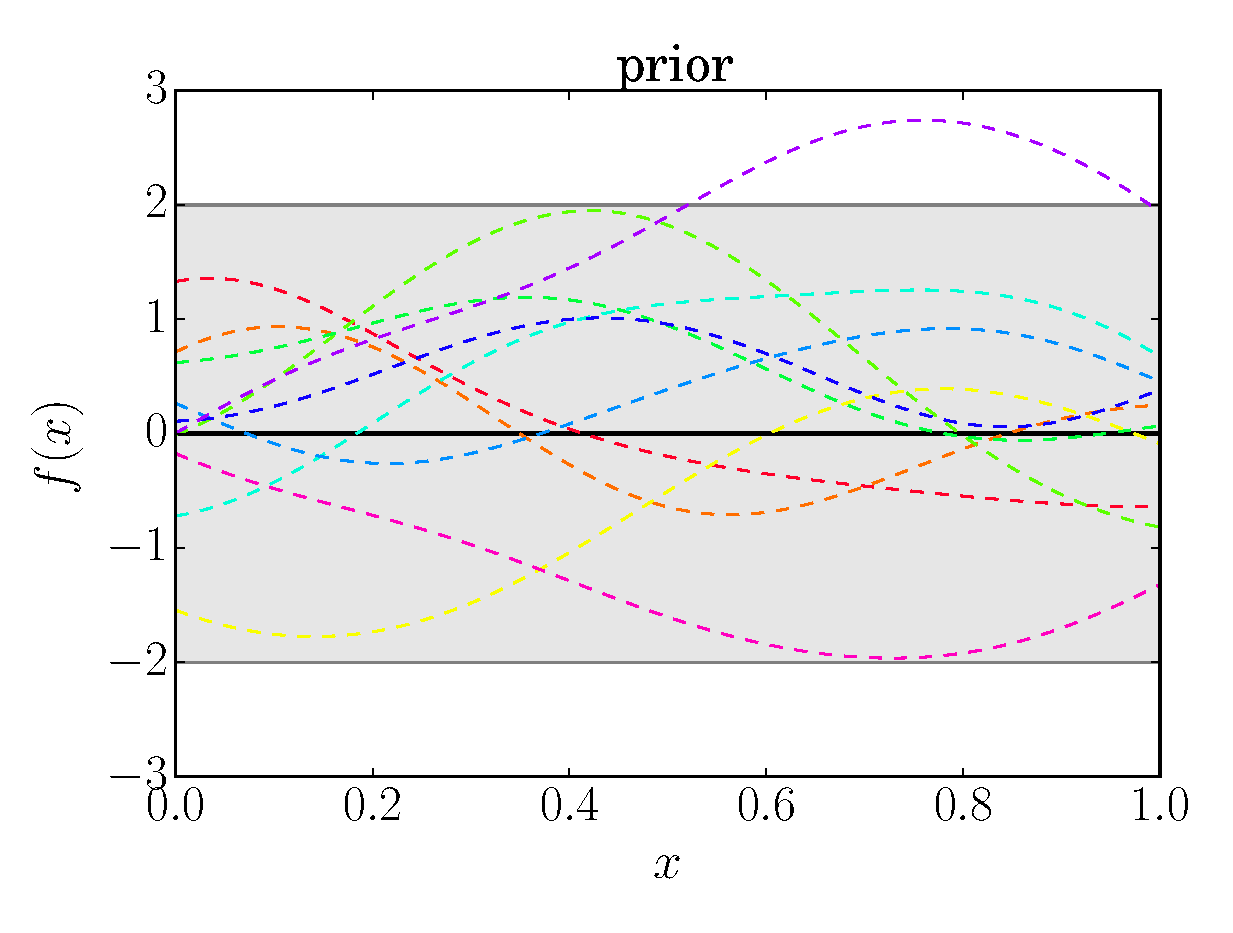
\includegraphics[width=0.48\textwidth]{Figures/bayesian_modeling/prior_draws.eps}
					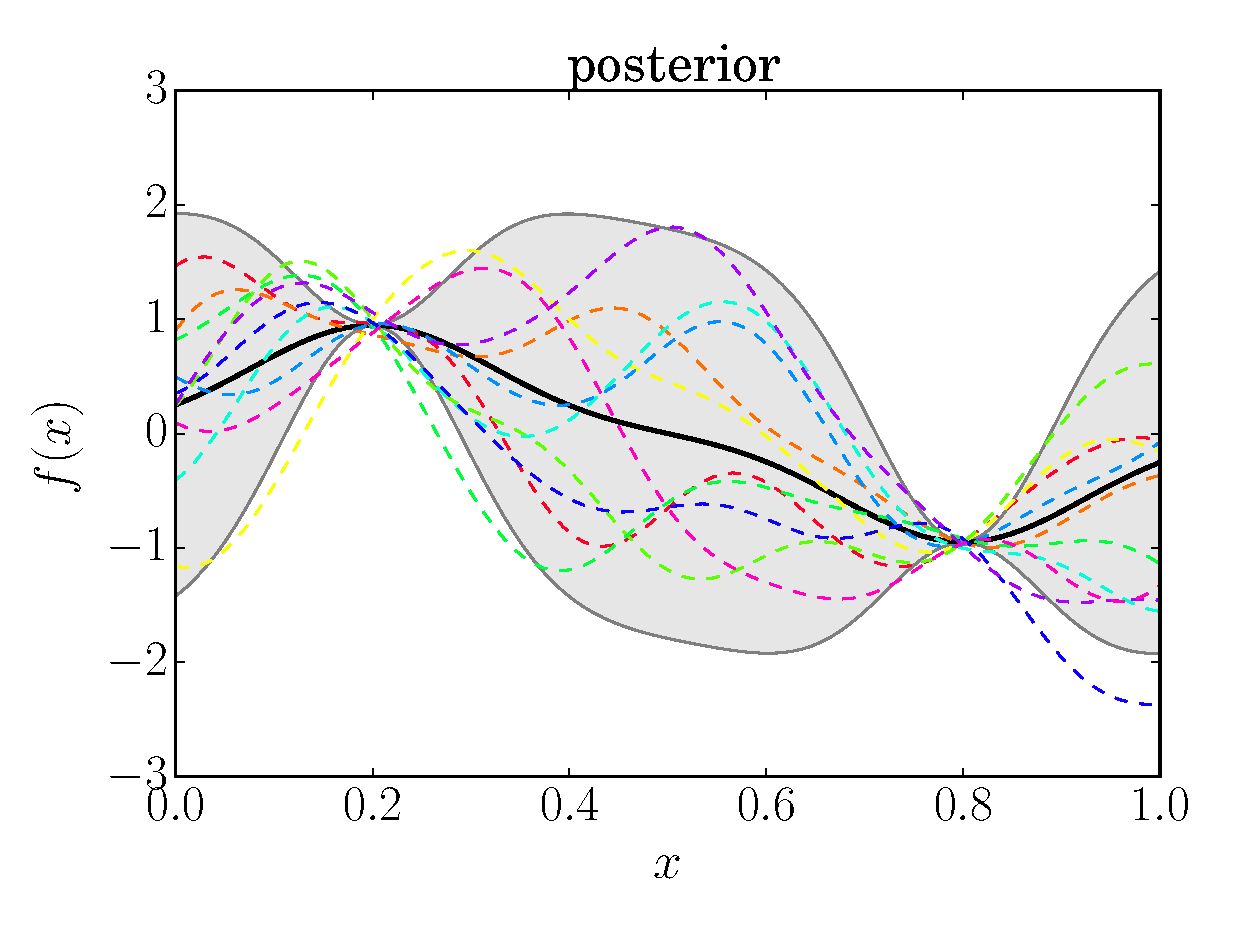
\includegraphics[width=0.48\textwidth]{Figures/bayesian_modeling/posterior_draws2.eps}
				\caption{Illustration of Gaussian Process Bayesian Modeling}
				\label{Figure:BayesianModeling}
			\end{figure}
			
			From this illustration, there are a few qualities one can notice. Firstly, the prior distribution is simply the zero function. The prior is meant to represent the system's current belief before the next observations are to be made. In this case, the prior situation involves no observations at all. Ideally, this means that the prior distribution should contain no predictive information. However, it is of philosophical note that all informative \footnote{It is certainly possible to perform inference without any assumptions. It will simply be uninformative in prediction or result.} inferences must begin with some assumptions regarding the structure of the phenomenon to be inferenced. In the illustration above, the function is assumed to be distributed as a process with zero mean. This assumption has excluded processes without means, such as the Cauchy process, as well as assumed a rather arbitrary mean function. However, this assumption is often valid as one can always pre-process the output data set through subtracting off their empirical mean so that the output is approximately distributed about zero. The representation of the standard deviation and hence variance as confidence bounds centred at the mean function also means that multi-model processes are excluded. For a Gaussian process, which is indeed uni-modal and have finite moments for all moments of finite degree, this illustration is common and useful for visualising the Bayesian modeling process. It is customary to visualise the 2-$\sigma$ bound for a Gaussian process. So, for this example, the prior distribution has a uniform standard deviation of one everywhere.
			
			Regarding the variance, a second observation is that the standard deviation and hence variance of the output function decreases at the observations, and gradually increases away from the observations. This leads to two remarks. Firstly, the variance or uncertainty of the output function at a location reduces when observations are made at that location. Secondly, neighboring points are related - the closer they are, the more related they are. This is seen through the observed points dragging nearby points towards it while reducing the uncertainty of nearby points. This resembles the concept of covariance. Evidently, points closer to each other have higher covariance then those further away, and the covariance beween the same points simply become its variance.
			
			The two observations above demonstrate that, just as a Gaussian distribution is defined through a mean vector and a covariance matrix, a Gaussian process is defined through a mean function $m(x)$ and a covariance function $k(x, x')$. In Gaussian process literature, the covariance function is also called a \textit{kernel} function.
			
			With an intuition of Gaussian processes in the Bayesian modeling context, a formal definition of Gaussian processes can now be introduced. In this thesis, the shorthand notation $I_{n} := \{1, 2, \dots, n\}$ will be used for concise indexing unless otherwise indicated, and is not to be confused with identity matrices $I_{p \times p} \in \mathbb{R}^{p \times p}$.
			
			\newpage
			\newtheorem{gpdef}{Gaussian Process}[section]
			\begin{gpdef}
				A random function $f(x)$, $x \in \mathbb{R}$, is distributed as a Gaussian process with mean function $m(x)$ and covariance function $k(x, x')$, if for any finite collection of feature points $\bvec{x} := [x_{1}, x_{2}, \dots, x_{n}]^{T}$, the corresponding output targets $\bvec{f}(\bvec{x}) := \{f(x_{i})\}_{i \in I_{n}} := [f(x_{1}), f(x_{2}), \dots, f(x_{n})]^{T}$ is jointly multivariate Gaussian distributed such that 

					\begin{equation}
						\bvec{f}(\bvec{x}) \sim \mathcal{N}(\bvec{m}(\bvec{x}), K(\bvec{x}, \bvec{x}'))
					\label{Equation:GaussianProcessFiniteDistribution}
					\end{equation}	
				
				where $\bvec{m}(\bvec{x}) :=  \{m(x_{i})\}_{i \in I_{n}} \in \mathbb{R}^{n}$ and $K(\bvec{x}, \bvec{x}') := \{k(x_{i}, x_{j})\}_{i \in I_{n}, j \in I_{n}}$. Such a function $f(x)$ is then notated as
				
					\begin{equation}
						f(x) \sim \mathcal{GP}(m(x), k(x, x'))
					\label{Equation:GaussianProcess}
					\end{equation}	
					
			\label{Definition:GaussianProcess}
			\end{gpdef}
			
			Certainly, this definition generalises finite dimensional multivariate Gaussian distributions, in that any subset of a multivariate Gaussian distributed random vector is also a multivariate Gaussian distributed of lower dimensionality.

			Definition \ref{Definition:GaussianProcess} is defined for a univariate input feature $x$. In fact, this definition generalises naturally to a multivariate input feature $\bvec{x} \in \mathbb{R}^{p}$ with $p$ features. This motivates definition \ref{Definition:GaussianRandomField}.
			
			\newtheorem{grfdef}{Gaussian Random Field}[section]
			\begin{grfdef}
				A random function $f(\bvec{x})$, $\bvec{x} \in \mathbb{R}^{p}$, is distributed as a Gaussian random field with mean function $m(\bvec{x})$ and covariance function $k(\bvec{x}, \bvec{x}')$, if for any finite collection of feature points $X := [\bvec{x}_{1}, \bvec{x}_{2}, \dots, \bvec{x}_{n}]^{T}$, the corresponding output targets $\bvec{f}(X) := \{f(\bvec{x}_{i})\}_{i \in I_{n}} := [f(\bvec{x}_{1}), f(\bvec{x}_{2}), \dots, f(\bvec{x}_{n})]^{T}$ is jointly multivariate Gaussian distributed such that 

					\begin{equation}
						\bvec{f}(X) \sim \mathcal{N}(\bvec{m}(X), K(X, X'))
					\label{Equation:GaussianRandomFieldFiniteDistribution}
					\end{equation}	
				
				where $\bvec{m}(X) :=  \{m(\bvec{x}_{i})\}_{i \in I_{n}} \in \mathbb{R}^{n}$ and $K(X, X') := \{k(\bvec{x}_{i}, \bvec{x}_{j})\}_{i \in I_{n}, j \in I_{n}}$. Such a function $f(\bvec{x})$ is then notated as
				
					\begin{equation}
						f(\bvec{x}) \sim \mathcal{GRF}(m(\bvec{x}), k(\bvec{x}, \bvec{x}'))
					\label{Equation:GaussianRandomField}
					\end{equation}	
					
			\label{Definition:GaussianRandomField}
			\end{grfdef}
			
			Notice that while Gaussian random fields describe the case for multivariate features, in practice the term is seldom used, and instead are also referred to as Gaussian processes. As such, it is conventional to simply write \eqref{Equation:GaussianRandomField} as \eqref{Equation:GaussianRandomFieldProcess}.
	
				\begin{equation}
					f(\bvec{x}) \sim \mathcal{GP}(m(\bvec{x}), k(\bvec{x}, \bvec{x}'))
				\label{Equation:GaussianRandomFieldProcess}
				\end{equation}	
							
			Finally, as mentioned before, the mean function can be generally assumed to be the zero function, as at each stage of inference both the model and data can be subtracted by their theoretical or empirical means. This elucidates that Gaussian processes are completely defined by their covariance function $k$. The covariance function $k$ is also refered to as the \textit{kernel} function. The next section will discuss the kernel function in detail.
			
			\FloatBarrier
			
		\subsection{Kernel Functions}
		\label{Background:GaussianProcesses:KernelFunctions}

			As kernel functions completely define the prediction and inference characteristics of a Gaussian process, this section aims to provide the mathematical background regarding kernels that are necessary for understanding Gaussian processes. The following discussion will only cover the minimal background necessary for further sections, as treatments of kernel functions can easily become very detailed and rigorous in topics such as differentiability effects or eigenfunction decomposition. Further treatment of this material is available through \cite{GaussianProcessForMachineLearning}. 
			
			Intuitively, the kernel function determines the \textit{similarity} between data points. This is a notion that all supervised learning algorithms intend to do, although rather implicitly in most cases. The GP formulation makes this explicit through the covariance between any two points in the feature space.
			
			Kernel functions can be categorised into stationary kernels and non-stationary kernels.
						
			\subsubsection{Stationary Kernels}
			\label{Background:GaussianProcesses:KernelFunctions:Stationary}
			
				Stationary kernels are ones whose covariance properties do not depend explicitly on the locations $\bvec{x}$ and $\bvec{x}'$ of consideration, but only on the difference $\bvec{x} - \bvec{x}'$ between them. Thus, the covariance properties are \textit{stationary}, or invariant, under translations in the feature space.
				
				Common stationary kernels are the squared exponential kernel \footnote{Squared exponential kernels are also sometimes called Gaussian kernels. However, in conversations it tends to create confusion between the probability density function $\phi(x)$ for Gaussian distributions and the covariance function $k(x, x')$ itself, so this term is avoided in this thesis.} and the \matern kernels, both of which belongs to the class of \textit{radial basis function} kernels. The squared exponential (SE) kernel between any two points $\bvec{x}, \bvec{x}' \in \mathbb{R}^{p}$ in the feature space with $p$ features has the following form \eqref{Equation:SquaredExponentialKernel}.
				
				\begin{equation}
					\left.
						\begin{aligned}
							k_{\mathrm{SE}}(\bvec{x}, \bvec{x}') &= \sigma_{f}^{2} \exp\Big(-\frac{1}{2}(\bvec{x} - \bvec{x}')^{T} \Sigma^{-1} (\bvec{x} - \bvec{x}')\Big) = \sigma_{f} \exp\Big(-\frac{1}{2} a^{2} \Big) \\
							\Sigma &= 	\begin{bmatrix}
											l_{1}^{2} & l_{12} & \dots & l_{1p} \\
											l_{21}^{2} & l_{2}^{2} & \dots & l_{2p} \\
											\vdots & \vdots  & \ddots & \vdots \\
											l_{p1}^{2} & l_{p2} & \dots & l_{p}^{2} \\
									  	\end{bmatrix}
						\end{aligned}
					\qquad \right.
				\label{Equation:SquaredExponentialKernel}
				\end{equation}
				
				Here, $\sigma_{f}$ is called the sensitivity, and determines the overall reference strength scale of the covariance function. The matrix $\Sigma$ is the length scale matrix, and determines the reference length scale and principle axis directions within the feature space. Like most quadratic forms, $\Sigma$ is required to be symmetric and positive semi-definite. In particular, when $\Sigma$ is diagonal, the kernel is termed \textit{axis aligned}. When $\Sigma$ is proportional to an identity such that $\Sigma = l^{2} I_{p \times p}$, the kernel is termed \textit{isotropic}.
				
				The sensitivity parameter $\sigma_{f}$ and length scale parameters $l_{ij}$, $i, j \in {1, 2, \dots, m}$ with $l_{i} := l_{ii}$ completely contain the information of a squared exponential kernel. Unlike parametric models, however, while these parameters define the kernel directly, they define the GP model indirectly. Because of the multiple levels of relation from these parameters to the model, these parameters are termed \textit{hyperparameters} of the GP.
				
				In practice, it is often possible to pre-process the data or transform the feature space so that an axis aligned kernel can be applied. The assumption imposed is that the principle axis directions are aligned with the feature space axis. In this case, the GP model is defined by $p + 1$ hyperparameters, where $p$ is the number of features. Without the axis-aligned structure, the number of hyperparameters is $\frac{p(p + 1)}{2} + 1$.
				
				The above formulation suggests to define $a^{2} := (\bvec{x} - \bvec{x}')^{T} \Sigma^{-1} (\bvec{x} - \bvec{x}')$. This can be interpreted as the squared distance between $\bvec{x}$ and $\bvec{x}'$ under the warp defined by $\Sigma$. In particular, when the feature space is isotropic such that $\Sigma = l^{2} I_{m \times m}$, then $a = \frac{r}{l}$ where $r := +\sqrt{r^{2}}$, $l := +\sqrt{l^{2}}$, and $r^{2} = (\bvec{x} - \bvec{x}')^{T} (\bvec{x} - \bvec{x}')$. In fact, most stationary kernels are functions solely of $a^{2}$, or with the definition $a := +\sqrt{a^{2}}$, they are simply scalar functions of scalar inputs $a = a (\bvec{x}, \bvec{x'})$. This form also makes evident that the covariances between two points decreases monotonically as the distance between them increases - a property most kernel functions exhibit. In fact, this structure characterises the \textit{radial basis function} class of kernels, and is the primary type of kernel relevant to this thesis.
				
				Continuing with this formulation, the \matern class of kernel functions are given by \eqref{Equation:MaternKernel}.
				
				\begin{equation}
					\left.
						\begin{aligned}
							k_{\mathrm{\maternmath}}(\bvec{x}, \bvec{x}') =& \; \sigma_{f}^{2} \frac{2^{1 - \nu}}{\Gamma(\nu)} \Big( \sqrt{2 \nu} a \Big)^{\nu} K_{\nu}\Big( \sqrt{2 \nu} a \Big) \\
							a^{2} :=& \; (\bvec{x} - \bvec{x}')^{T} \Sigma^{-1} (\bvec{x} - \bvec{x}')
						\end{aligned}
					\qquad \right.
				\label{Equation:MaternKernel}
				\end{equation}
							
				Here, $\Gamma$ and $K_{\nu}$ are the Gamma function and modified Bessel function respectively, while $\nu$ is a positive hyperparameter that determines the differentiability property of the \matern class kernel. The GP model with \matern class kernel is $d$-times mean square differentiable if and only if $\nu > d$ \citep{GaussianProcessForMachineLearning}. In the limit of $\nu \rightarrow \infty$ for infinite differentiability, the \matern kernel becomes the squared exponential kernel \eqref{Equation:SquaredExponentialKernel}. While the general \matern class kernel seem complicated due to the Gamma function and modified Bessel function, its form become simple for $\nu = p + \frac{1}{2}$ where $p$ is a non-negative integer. That is, \matern kernels with $\nu = \frac{1}{2}, \frac{3}{2}, \frac{5}{2}, \frac{7}{2}, \dots$ have simple analytic forms without reference to the modified Bessel function. In fact, for $\nu > \frac{5}{2}$, the degree for which the \matern kernel changes becomes quite unnoticeable for most practical purposes such that it may as well be replaced by the squared exponential kernel with $\nu \rightarrow \infty$. Similarly, while there is a more noticeable effect of changing $\nu$ within the range $\nu \in (0, \frac{5}{2})$, in practice is it is often not worth the expense of implementing the complicated form for a almost unnoticeable improvement in modeling accuracy. Hence, it is replaced with the \matern kernel with $\nu = \frac{1}{2}, \frac{3}{2}, \frac{5}{2}$, whichever is the closest. In this way, in practice only the \matern kernels with $\nu = \frac{1}{2}, \frac{3}{2}, \frac{5}{2}$ are employed, and they are respectively termed the \matern 1/2 kernel, \matern 3/2 kernel, and \matern 5/2 kernel - in the order of increasing differentiability. These kernels have the forms listed below \eqref{Equation:PracticalMaternKernels}.
				
				\begin{equation}
					\left.
						\begin{aligned}
							k_{\mathrm{\maternmath}, \; \nu = \frac{1}{2}}(\bvec{x}, \bvec{x}') =& \; \sigma_{f}^{2} \exp ( -a ) \\
							k_{\mathrm{\maternmath}, \; \nu = \frac{3}{2}}(\bvec{x}, \bvec{x}') =& \; \sigma_{f}^{2} (1 + \sqrt{3} a) \exp ( -\sqrt{3} a ) \\
							k_{\mathrm{\maternmath}, \; \nu = \frac{5}{2}}(\bvec{x}, \bvec{x}') =& \; \sigma_{f}^{2} \Big(1 + \sqrt{5} a + \frac{5}{3} a^{2}\Big) \exp ( -\sqrt{5} a )  \\
							a^{2} :=& \; (\bvec{x} - \bvec{x}')^{T} \Sigma^{-1} (\bvec{x} - \bvec{x}')
						\end{aligned}
					\qquad \right.
				\label{Equation:PracticalMaternKernels}
				\end{equation}			
				
				Together, the squared exponential kernel and the \matern class kernels provide a flexible set of kernel functions that can model a multitude of phenomena from various fields such as geology, ecology, finance, logistics, control theory, and machine learning.
			
			\subsubsection{Non-Stationary Kernels}
			\label{Background:GaussianProcesses:KernelFunctions:Nonstationary}
			
				Non-stationary kernels introduce flexibility for modeling phenomenons where the inherent length scales varies across feature locations. The limitations with stationary kernels is that the GP will always learn length scales that are as small as it needs to be for modeling the fastest varying phenomenon in the model. While the marginal likelihood inherently balances modeling accuracy and overfitting, when it comes to the choice between modeling a peak in data variation with a risk of overfitting the rest of the data or ignoring that peak, the optimiser will always prefer the former as marginal likelihood gain from successful modeling is higher than loss from overfitting. Because learning stage is done through optimising the marginal likelihood (see section \ref{Background:GaussianProcess:Regression:HyperparameterLearning}), this forces the length scale to be smaller than it needs at slower varying places.

				Figure \ref{Figure:GaussianProcessLengthScale} illustrates the non-stationary Gaussian process for a terrain modeling application, where flat regions have high length scales (slow varying) while rough regions have low length scales (fast varying). Note that this does not imply that it is only relevant for GP regression problems - the latent functions used in GP classification is itself a GP regression problem for which length scale interpretation is almost identical to that shown in \cref{Figure:GaussianProcessLengthScale} (see section \ref{Background:GaussianProcesses:Classification}).
				
				\begin{figure}[!htbp]
					\centering
						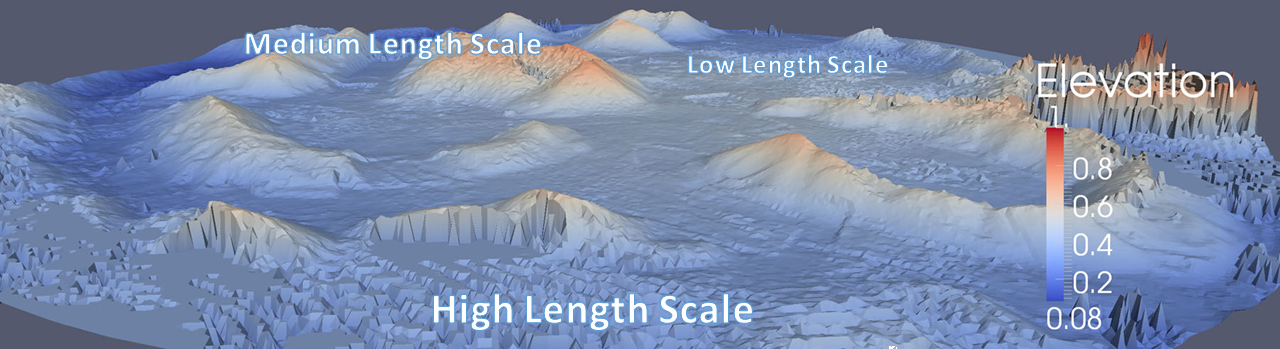
\includegraphics[width=\textwidth]{Figures/gaussianprocesslengthscale.png}
					\caption{Non-stationary Gaussian process for seafloor terrain modeling Adapted from \cite{ROB:ROB21403}}
					\label{Figure:GaussianProcessLengthScale}
				\end{figure}
				
				The non-stationary kernel function employed in this thesis is the Paciorek non-stationary covariance kernel function \eqref{Equation:NonStationaryKernel} \citep{AdaptiveNonStationaryKernel}.
				
				\begin{equation}
					k(\bvec{x}_{i}, \bvec{x}_{j}) = \sigma_{f}^{2} |\Sigma_{i}|^{\frac{1}{4}} |\Sigma_{j}|^{\frac{1}{4}} \Bigg|\frac{\Sigma_{i} + \Sigma_{j}}{2}\Bigg|^{-\frac{1}{2}} \exp\Bigg[ -\frac{1}{2} (\bvec{x}_{i} - \bvec{x}_{j}) \Bigg(\frac{\Sigma_{i} + \Sigma_{j}}{2}\Bigg)^{-1} (\bvec{x}_{i} - \bvec{x}_{j}) \Bigg]
				\label{Equation:NonStationaryKernel}
				\end{equation}			
				
				The matrices $\Sigma_{i}$ and $\Sigma_{j}$ are the local length scale matrices at $\bvec{x}_{i}$ and $\bvec{x}_{j}$ respectively, and are interpreted the same way as the stationary case. The only difference is that these length scale matrices only operate locally, and are functions of the input feature vector $\bvec{x}$. In each kernel location, two length scale matrices are queried. Hence, in a kernel matrix of size $n \times m$, maximally $n + m$ unique queries are made if no feature locations overlap.
				
				It is worthwhile to observe that the effective length scale matrix in the exponent is the average of the two length scale matrices, with its effect reduced with increasing distance between the two points of consideration as with all kernels.
				
				Note that the normalisation matrix determinants are chosen such that the kernel function is reduced into the squared exponential stationary kernel when $\Sigma_{i} = \Sigma_{j} = \Sigma$, as derived in \eqref{Equation:NonStationaryKernelToStationaryKernel}. 
		
				That is, the Paciorek non-stationary kernel reduces to the squared exponential kernel under the stationary limit. In this way, the Paciorek kernel generalises the squared exponential kernel.
						
				\begin{equation}
					\left.
						\begin{aligned}
							k(\bvec{x}_{i}, \bvec{x}_{j}) &= \sigma_{f}^{2} |\Sigma|^{\frac{1}{4}} |\Sigma|^{\frac{1}{4}} \Bigg|\frac{\Sigma + \Sigma}{2}\Bigg|^{-\frac{1}{2}} \exp\Bigg[ -\frac{1}{2} (\bvec{x}_{i} - \bvec{x}_{j}) \Bigg(\frac{\Sigma + \Sigma}{2}\Bigg)^{-1} (\bvec{x}_{i} - \bvec{x}_{j}) \Bigg] \\
							&= \sigma_{f}^{2} |\Sigma|^{\frac{1}{2}} |\Sigma|^{-\frac{1}{2}} \exp\Bigg[ -\frac{1}{2} (\bvec{x}_{i} - \bvec{x}_{j}) (\Sigma)^{-1} (\bvec{x}_{i} - \bvec{x}_{j}) \Bigg] \\
							&= \sigma_{f}^{2} \exp\Bigg[ -\frac{1}{2} (\bvec{x}_{i} - \bvec{x}_{j}) \Sigma^{-1} (\bvec{x}_{i} - \bvec{x}_{j}) \Bigg]
						\end{aligned}
					\qquad \right.
				\label{Equation:NonStationaryKernelToStationaryKernel}
				\end{equation}		
			
		\subsection{Regression}
		\label{Background:GaussianProcesses:Regression}
		
			Gaussian process regression is a regression technique that employs Gaussian processes as its inference model. Because Gaussian processes already operate on function spaces with continuous inputs and outputs, no extra pre-processing or transformations are needed. The bulk of the technique thus lies in learning the kernel function of the Gaussian process. Gaussian process regression is also called \textit{kriging} or Kolmogorov Wiener prediction when used for interpolating geospatial data in a geostatistics setting. This section attempts to summarise the important concepts regarding GP regression and how they work.
			
			Once a kernel function is chosen, such as the squared exponential or \matern kernels, learning the kernel function becomes equivalent to learning the hyperparameters of the kernel. In this way, the Gaussian process model is defined completely by its hyperparameters $\vec{\uptheta}$. % , which are often only handful in quantity. % This illustrates that while its temporal complexity $\mathcal{O}(n^{3})$ is quite high, its spatial complexity and memory requirements are quite moderate at $\frac{m(m + 1)}{2} + 1 + n(m  + 1)$ real numbers, where $n(m  + 1)$ real numbers comes from the training data itself. % Minimally, after assuming a particular kernel functional form, the bulk of the model information is held by the data set itself. Especially in big data applications, unlike generalised linear models and neural networks whose information vector \footnote{The information vector is the vector of all parameters that defines the model.} is proportional to the number of basis functions employed, a Gaussian process model can have its information stored by a few hyperparameters.
			
			Before presenting the inference process for Gaussian process regression however, it is important to understand the way Gaussian processes are used in general for Bayesian inference, which applies to both regression and classification.
			
			\subsubsection{General Gaussian Process Inference Process}
			
				The formulation for Gaussian processes from definitions \ref{Definition:GaussianProcess} and \ref{Definition:GaussianRandomField} provides an framework for inferring the behaviour of an unknown function $f(\bvec{x})$. In general, however, the output target does not have to be the functional outputs $f := f(\bvec{x})$. Instead, the output targets are some quantity $y$ which can be directly observed and recorded. The function $f$ serves as an intermediate step to infer $y$ from $\bvec{x}$, and in general cannot be directly observed. Therefore, the function $f$ is also called the \textit{latent function}.
				
				% Define block styles
				\tikzstyle{line} = [draw, -latex']
				\tikzstyle{cloud1} = [draw, ellipse, fill = green!30!blue!30, node distance = 3cm, minimum height = 3em,  minimum width = 5em]
				\tikzstyle{cloud2} = [draw, ellipse, fill = green!60!blue!50, node distance = 3cm, minimum height = 3em,  minimum width = 5em]
				
				\begin{figure}[!ht]
				\centering\makebox[\textwidth]{
					\begin{tikzpicture}[node distance = 4cm, auto, comment/.style ={rectangle, inner sep = 2pt, text width = 4cm, }]
					
					\node [cloud1] (trainingfeatures) {$X$};
					\node [cloud2, right of = trainingfeatures] (traininglatents) {$\bvec{f}$};
					\node [cloud1, right of = traininglatents] (trainingtargets) {$\bvec{y}$};
					\node [cloud2, below of = traininglatents] (querylatents) {$\bvec{f}^{\star}$};
					\node [cloud1, left of = querylatents] (queryfeatures) {$X^{\star}$};
					\node [cloud2, right of = querylatents] (querytargets) {$\bvec{y}^{\star}$};
					
					\draw [line] (trainingfeatures) -- (traininglatents);
					\draw [line] (traininglatents) -- (trainingtargets);
					\draw [line] (traininglatents) -- (querylatents);
					\draw [line] (queryfeatures) -- (querylatents);
					\draw [line] (querylatents) -- (querytargets);	
					\end{tikzpicture}
					}		
				\caption{Gaussian Process Graphical Model}
				\label{Figure:GaussianProcessGraphicalModel}
				\end{figure}
				
				This inference process can be visualised with the graphical model presented in Figure \ref{Figure:GaussianProcessGraphicalModel}. Observed and known quantities are coloured in blue. Quantities to be inferred are coloured in green. Note that in a Bayesian model, the unknown quantities (in green) are inferenced by their probabilistic distributions, and not just their estimated values.
				
				Latent functions are usually interpreted as the underlying phenomenon which stochastically generates the target outputs $y$.  The model assumes that a particular phenomenon $f$ is responsible for generating the output target $y$, and that the phenomenon $f$ can be explained reasonably by a particular set of features $\bvec{x}$. A collection of output targets $\bvec{y}$ and corresponding features $X$ are observed. The collected dataset $(X, \bvec{y})$ is termed the \textit{training data}. A \textit{learning process} then occurs where the model learns the underlying phenomenon $\bvec{f}$ at the training points. If the learning process is done through an optimisation procedure in search for an optimal model in some quantifiable sense, the learning process is also termed a \textit{training process}. An \textit{inference process} then occurs where the model is to infer the latent process $\bvec{f}^{\star}$ at the query features $X^{\star}$, which would further allow inference on the corresponding target outputs $\bvec{y}^{\star}$. The inference process in general also includes the act of inferring related quantities regarding the distribution of $\bvec{y}^{\star}$. Typical examples include inferring the uncertainty involved in the inference stage through a variance or entropy measure. If the only quantity to be inferenced is the expected target outputs $\mathbb{E}[\bvec{y}^{\star} | \bvec{y}]$, then the inference process is also termed a \textit{prediction process}. In this way, the GP modeling process is composed of two stages - the learning or training stage and the inference or prediction stage.
				
				A typical example in the regression case is a situation where the observable outputs $y$ are related to the underlying phenomenon $f(x)$ through a simple white noise process \eqref{Equation:RegressionNoiseModelScalar}.
				
				\begin{equation}
					y_{i} = f(\bvec{x}_{i}) + \epsilon_{i} \qquad \epsilon_{i} \sim \mathcal{N}(0, \sigma^{2}) \qquad \forall i \in I_{n}
				\label{Equation:RegressionNoiseModelScalar}
				\end{equation}
				
				In general, however, the relationship between the output target $y$ and the latent functional $f$ is captured through a likelihood response $p(y | f)$, which captures the likelihood of generating a particular output target $y$ \textit{if} the latent functional is $f$. In fact, the choice of the likelihood function is not immediately straightforward and is of vital importance in the classification scenario. 
				
				In the regression model above \eqref{Equation:RegressionNoiseModelScalar}, a degenerate case arises when the noise level $\sigma$ is zero such that $y = f$ everywhere. In this case, $p(y | f) = p(f | f) = 1$ such that the Gaussian process model performs inference on the target output directly through obtaining $p (y) = p(f)$. When this is not the case, however, the quantity to be inferred in the end is the output targets $y$. As such, the distribution of interest is $p(y)$. This can be obtained by marginalising away the latent functionals $f$ over the likelihood $p(y | f)$ \eqref{Equation:Marginalisation}.
				
				\begin{equation}
					p(y) = \int_{\mathscr{F}} p(y | f) p(f) df
				\label{Equation:Marginalisation}
				\end{equation}
				
				where $\mathscr{F}$ is the space of all latent functionals. Note that the form \eqref{Equation:Marginalisation} above is written in functional form to illustrate the relevant concepts. The marginalisation process above plays a vital process in the learning stage for Gaussian process inference discussed shortly.
		
			\subsubsection{Inference}
			
				The above general inference process can now be formulated specifically for the regression case.
				
				With a given kernel function $k$ as the covariance function, by definition \ref{Definition:GaussianRandomField} we have that the training latents $\bvec{f}$ and the query latents $\bvec{f^{\star}}$ are distributed as a multivariate Gaussian \eqref{Equation:InferenceJointDistribution}.
				
				\begin{equation}
					\begin{bmatrix}
						\bvec{f^{ }} \\ \bvec{f^{\star}}
					\end{bmatrix}
					\sim \mathcal{N}\Bigg(\bvec{0}, \begin{bmatrix}
														K(X, X) & K(X, X^{\star}) \\
														K(X^{\star}, X) & K(X^{\star}, X^{\star}) \\
													\end{bmatrix}  \Bigg)
				\label{Equation:InferenceJointDistribution}
				\end{equation}
				
				% where the matrix $K(X, X')$ is defined to have elements $K_{ij} = k(\bvec{x}_{i}, \bvec{x}'_{j})$ with $X$ and $X'$ defined as the canonical data design matrix form \eqref{Background:GaussianProcess:Equation:DataMatrix}, both of each can take either the matrix of training points $X$ of size $n$ or query points $X^{\star}$ of size $n^{\star}$.
				
				To shorten notation, it is customary to define $K := K(X, X)$, $K^{\star} := K(X, X^{\star})$, $K^{\star \star} := K(X^{\star}, X^{\star})$, where the symmetry of the covariance matrix readily yields ${K^{\star}}^{T} := K(X^{\star}, X)$. In this thesis, $K$ will be referred to as the \textit{data kernel} or \textit{training kernel}, $K^{\star}$ as the \textit{inference kernel}, and $K^{\star \star}$ as the \textit{query kernel}.
				
				\begin{equation}
					X = \{\bvec{x}_{i}\}_{i \in I_{n}}^{T} := \begin{bmatrix}
						\bvec{x}_{1}^{T} \\ \bvec{x}_{2}^{T} \\ \dots \\ \bvec{x}_{n}^{T}
					\end{bmatrix} \qquad X' = \{\bvec{x'}_{i}\}_{i \in I_{n}}^{T} := \begin{bmatrix}
										\bvec{x'}_{1}^{T} \\ \bvec{x'}_{2}^{T} \\ \dots \\ \bvec{x'}_{n}^{T}
									\end{bmatrix}
				\label{Equation:TrainingQueryDataMatrices}
				\end{equation}	
					
				The joint distribution readily contains information for the conditional distribution of the query points given the training points $p(\bvec{f^{\star}} | \bvec{f})$ knowing the training points and query locations. This leads to the posterior distribution \eqref{Equation:InfereceConditionalDistribution}. Note that in some literature, the feature locations $X$ and $X^{\star}$ are also included in the conditioned set, so that the conditional distribution is written as $\bvec{f^{\star}} | \bvec{f}, X, X^{\star}$. However, throughout this thesis, since the feature locations $X$ and $X^{\star}$ are always known, they are inherently conditioned upon and will not be shown explicitly in notation for consise presentation. 
				
				\begin{equation}
					\bvec{f^{\star}} | \bvec{f} \sim \mathcal{N}({K^{\star}}^{T} K^{-1} \bvec{f}, K^{\star \star} - {K^{\star}}^{T} K^{-1} K^{\star})
				\label{Equation:InfereceConditionalDistribution}
				\end{equation}						
				
				A comparison with the prior $\bvec{f^{\star}} \sim \mathcal{N}(\bvec{0}, K^{\star \star})$ shows the mean effect ${K^{\star}}^{T} K^{-1} \bvec{f}$ and covariance effect $- {K^{\star}}^{T} K^{-1} K^{\star}$ which introduces observed information into the model. Interestingly, as ${K^{\star}}^{T} K^{-1} K^{\star}$ is positive definite, this intuitively means that the observation has reduced uncertainty in the model.
				
				The above posterior formulation encompasses the heart of the GP regression model. The rest of the discussion will focus on detailed aspects of its implementation and variants.
				
				% \subsubsection{Noisy Observations}
				
				Under noisy observations, a hyperparameter $\sigma$ is introduced for the standard deviation of the noise, which is also assumed to be \textit{iid} and Gaussian distributed with standard deviation $\sigma$ and zero mean. The only alteration is the observations are notated as $\bvec{y}$ instead of $\bvec{f}$, where 
				
				\begin{equation}
					\bvec{y}(X) = \bvec{f}(X) + \bvec{\upepsilon} \qquad \bvec{\upepsilon} \sim \mathcal{N}(\bvec{0}, \sigma^{2} I_{n \times n})
				\label{Equation:RegressionNoiseModel}
				\end{equation}
							
				and most importantly the data kernel is to be replaced with $K \mapsto K + \sigma^{2} I$. Note that however the query points remain as the latent function $\bvec{f^{\star}}$. If one were to predict future observations $\bvec{y^{\star}}$, then it suffices to generate $\bvec{f^{\star}}$ from the posterior and add randomly generated noise with standard deviation $\sigma$.
				
			\subsubsection{Hyperparameter Learning}
			\label{Background:GaussianProcess:Regression:HyperparameterLearning}
			
				One of the most important yet tricky aspects of GP modeling is the training stage. Since the model is determined entirely by the hyperparameters, the hyperparameters must be optimised in accordance to some fitness metric. The fitness metric employed to be maximised is the marginal likelihood, otherwise termed as evidence, of the observed data. This is usually non-trivial to compute and, in most cases, analytical forms do not exist. Fortunately, due to the Gaussian structure of the GP model, there exists an analytical form for the marginal likelihood. In practice, however, it is computationally faster to compute the log marginal likelihood \eqref{Background:GaussianProcess:Equation:LogMarginalLikelihood}.
				
				\begin{equation}
					\log(p(\bvec{f})) = - \frac{1}{2} \bvec{f}^{T} K^{-1} \bvec{f} - \frac{1}{2} \log|K| - \frac{n}{2} \log(2 \pi)
				\label{Background:GaussianProcess:Equation:LogMarginalLikelihood}
				\end{equation}
				
				Again, with noisy observations, corresponding substitutions with the data kernel matrix $K \mapsto K + \sigma^{2} I$ and observations $\bvec{f} \mapsto \bvec{y}$ is to be made.
				
				The last term is a constant, so it can be ignored during the optimisation stage and included back in once optimisation completes.
				
				In practice, hyperparameter learning can be sped up by employing the fact that $\frac{1}{2} \log|K| = \sum_{i} L_{ii} = \mathrm{trace}(L)$ where $L$ is the Cholesky decomposition of $K$ (or $K + \sigma^{2} I$ in the noisy case). In fact, the Cholesky decomposition $L$ leads to better numerical stability when inverting the matrix $K$ since $K = LL^{T}$ so that $K \backslash \bvec{y} = L^{T} \backslash (L \backslash \bvec{y})$.
				
		\subsection{Classification}
		\label{Background:GaussianProcesses:Classification}
		
			The GP classification method is of vital importance to the benthic habitat modeling process. It is used to distinguish and predict the environment type with a measure of entropy in order to quantify the information reward one can gain by exploring the area.
			
			Unlike the regression case, because the output labels are no longer continuous, it cannot be represented by a continuous probability density function such as a Gaussian. As such, a continuous latent function is introduced in the GP classification process. Intuitively, this latent function quantifies and measures the distinct qualities of the label. As a binary classification example, if the classifier is to distinguish between ``apples'' and ``oranges'', the latent function would then represent the ``appleness'' of each observation, with high ``appleness'' corresponding to observations likely to be ``apples'' and low ``appleness'' corresponding to observations likely to be ``oranges''. Note that only one latent function is needed in the binary case. The latent function is then monotonically ``squashed'' into the unit range [0, 1] so that it can be interpreted as a probability.
			
			Although the latent function is now continuous such that it is possible to model it with a GP regression model, the posterior probability is in general non-Gaussian distributed, since the ``squashing'' is usually non-linear such that the likelihood is non-Gaussian. In this way, approximations are necessary. Four of the most popular approximations to GP classification, in increasing accuracy and computational complexity, are Probabilistic Least Squares, Laplace Approximation, Expectation Propagation, and Variational Inference \citep{GaussianProcessForMachineLearning}. In this thesis, Laplace approximation is chosen as a reasonable balance between accuracy and implementation difficulty, although a short investigation of probabilistic least squares will also be provided.
			
			\subsubsection{Response Functions}
			\label{Background:GaussianProcesses:Classification:ResponseFunction}
			
				Before discussions begin regarding the various types of GP classifiers, it is important to understand the role of \textit{response functions} in Bayesian classifiers.
				
				The response function is sometimes also called a sigmoid function, and are used as the likelihood model for Bayesian classifiers. These functions must satisfy the requirement that is it monotonically non-decreasing with a domain of all real numbers $\mathbb{R}$ and a range of unit interval [0, 1]. That is, $\lambda(z): \mathbb{R} \mapsto [0, 1]$. As referenced above, these functions serve to "squeeze" the latent functions into a range where probabilistic interpretation is possible.
				
				The most widely used response functions are the logistic function \eqref{Equation:LogisticResponse} and probit \footnote{The probit function is also simply the standard normal cumulative distribution. The term \textit{probit} is used to make explicit its interpretation as a response likelihood function.} response \eqref{Equation:ProbitResponse} (figure \ref{Figure:LikelihoodResponses}).
				
				\begin{equation}
					\lambda(z) = \frac{1}{1 + \exp(-z)}
				\label{Equation:LogisticResponse}
				\end{equation}
				
				\begin{equation}
					\lambda(z) = \Phi(z) := \int\limits_{-\infty}^{z} \phi(x) dx =  \int\limits_{-\infty}^{z} \frac{1}{\sqrt{2 \pi}} \exp\Big(- \frac{1}{2} x^{2}\Big) dx
				\label{Equation:ProbitResponse}
				\end{equation}
			
				\begin{figure}[!htbp]
					\centering
						\includegraphics[width=0.75\textwidth]{Figures/responses.eps}
					\caption{Common likelihood responses}
					\label{Figure:LikelihoodResponses}
				\end{figure}
				
			\subsubsection{Binary Classification}
			\label{Background:GaussianProcesses:Classification:BinaryClassification}
			
				The Laplace approximation for GP binary classification works by learning a latent function through an iterative scheme involving successive GP regressions, and "squeezing" that latent function into an appropriate probabilistic range for likelihood interpretation. The Laplace approximation approaches the approximation problem by determining the mean and variance of the true distribution and approximating the said distribution with a Gaussian distribution of the same mean and variance. Assuming Gaussian distributions, the prior and the evidence (marginal likelihood) have analytical forms. Under such assumptions it is therefore possible to marginalise out the likelihood predictions to obtain a posterior estimate. Finally, this learning stage can be trained by optimising the marginal likelihood \footnote{{\color{BurntOrange} At this stage of the thesis progress, it is uncertain whether or not a deeper and more rigorous theoretical grounding should be provided for GP classification. Perhaps it would benefit by only providing an intuitive outline of the procedure, rather than a rigorous derivation, so that the reader is not distracted from the main contributions of this thesis later on.}}.
				
			\subsubsection{Laplace Approximation}
			\label{Background:GaussianProcesses:Classification:LaplaceApproximation}
			
			\subsubsection{Probabilistic Least Squares}
			\label{Background:GaussianProcesses:Classification:ProbabilisticLeastSquares}
			
			\subsubsection{Multiclass Classification: One v.s. All}
			\label{Background:GaussianProcesses:Classification:OVA}
			
				While a consistent framework for the GP Multi-class classification using Laplace approximation exist, a simpler and perhaps a more computationally efficient approach is to employ the One v.s. All (OVA) and All v.s. All (AVA) philosophy. The following discussion assumes that there are $c > 2$ classes of labels for which classification is to occur. 
				
				The OVA approach performs classification by introducing $c$ \textit{independent} classification problems, each trying to classify a label against all others. Each of these problems are thus a binary classification problem for which solution methods are known. Once the predictive probabilities from all learned GP classifiers are obtained, a consistent framework is used for fusing the separate prediction probabilities into a coherent prediction probability. This is necessary as the binary classifiers are independently learned and performs prediction independently, and may not necessarily provide coherent results. In fact, simply stacking the prediction probabilities together yields a "probability" distribution that does not sum up to 1.
				
				The AVA approach operates similarly. It insteads introduces $\frac{c (c - 1)}{2}$ \textit{independent} classification problems, each classifying between a pair of labels. The same exact philosophy follows in that a final consistent framework is needed for fusing the prediction probabilities into one coherent prediction probability. It is often more difficult for probability fusion in the AVA setting as compared to the OVA setting.
			
			\subsubsection{Multiclass Classification: All v.s. All}
			\label{Background:GaussianProcesses:Classification:AVA}
			
			\subsubsection{Fusion of Prediction Probability}
			\label{Background:GaussianProcesses:Classification:ProbabilityFusion}
			
				{\color{BurntOrange} This section should be in the GP implementation chapter of this thesis (e.g. Chapter 3). It would further the discussion above regarding the probability fusion problem by introducing the exclusion method and mode keeping method that has been developed and tested. It is anticipated that other methods will be developed by then, so that this section would undergo significant editing.}
				
				
				
	%				The main decision and analysis to be made in both the OVA and AVA setting is the framework for which the probabilities are to be fused. 
	%							
	%				The exclusion method centers around the idea that the probabilities are to be made consistent by eliminating, or excluding, the events that are impossible.
	%				
	%				Consider a single query point for which class prediction is to occur. Let $\pi_{i}$ be the prediction probability obtained through the binary classification of class $i$ against all other classes. Initially, the probability vector $\bvec{\pi} := [\pi_{1}, \pi_{2}, \dots, \pi_{c}]^{T}$ is not a unit vector, so that $\bvec{\pi}$ does not define a proper probability distribution \dots 
		
			\subsubsection{Entropy}
			\label{Background:GaussianProcesses:Classification:Entropy}
			
				After a predictive probability distribution is obtained for each query environment location, the uncertainty of such predictions can be quantified through the entropy of of that distribution.
				
				The output of a GP classifier is a discrete probability distribution with finite size - equal to the number of classes. For a general discrete probability distribution $p(x)$, the entropy is quantified as below \eqref{Equation:DiscreteEntropy} \cite{ShannonEntropy}.
				
				\begin{equation}
					H(p) = - \sum_{i} p(x_{i}) \log(p(x_{i}))
				\label{Equation:DiscreteEntropy}
				\end{equation}
				
				Although it is unlikely that the entropy of bathymetric feature modeling is required, the regression posterior is a continuous probability density $p(x)$ for which a similar form for distribution entropy exists \eqref{Equation:ContinuousEntropy}.
				
				\begin{equation}
					H(p) = - \int_{\Omega_{x}} p(x) \log(p(x)) dx
				\label{Equation:ContinuousEntropy}
				\end{equation}
								
				With these entropy measures, predictive uncertainties can be quantified, which allows active information seeking plans to be possible.
				
			\subsubsection{Sampling from a Gaussian Process for Classifiers}
			\label{Background:GaussianProcesses:Classification:Sampling}
			
	\section{Active Sampling}
	\label{Background:ActiveSampling}
	
		\subsection{Static Active Sampling}
		\label{Background:ActiveSampling:Static}
		
		\subsection{Dynamic Active Sampling}
		\label{Background:ActiveSampling:Dynamic}
		
	\section{Informative Path Planning}
	\label{Background:InformativePathPlanning}
	
		Path planning under dynamic uncertainty has been a challenging task for all information searching missions. This class of path planning problems have the special property that there is no goal location, and no stationary node, edge, or field cost to be cumulatively minimised. The objective is to reduce the overall uncertainty or entropy of a particular region given indefinite time. The complication is introduced with the non-linear dynamics of the uncertainty or entropy field of the region each time a planned path is executed, which also makes the solution extremely frequency dependent.
		
		Prior work and attempts at the active path planning problem include Marchant and Ramos (2014), where Bayesian Optimisation (BO) techniques combined with Gaussian process models are employed in an environmental monitoring setting \citep{BayesianOptimisation}. In this layered Bayesian Optimisation approach, two Gaussian processes are used - one to model the phenomenon and the other to model the quality of selected paths. Through Bayesian optimisation, sampling over continuous paths are optimised which maximises the reward over the final mission trajectory. The path planning process is done using Markov Decision Processes (MDP) with a Reinforcement Learning approach. Rapidly Exploring Random Graphs (RRGs) is combined with BO to search for informative paths. In this way, a continuous path can be planned through BO \citep{BayesianOptimisation}.
		
		This was was further extended by Marchant et. al. (2014) where Sequential Bayesian Optimisation (SBO) is used as online POMDPs for path planning \citep{SequentialBayesianOptimisation}.
		
		Other prior work includes Brooks et. al. (2006) where the POMDP approach is investigated for continuous state space planning \citep{ParametricPOMDP}. This method was compared to previous work with value-based and gradient-based solution methods which seek to transcribe the continuous problem into a discrete problem \footnote{{\color{BurntOrange} The author has practiced with transcribing the continuous problem into a discrete problem in a shortest path setting in}}. One of the most important limitations discussed in this work is that analytical and accurate solutions exist almost only for linear systems with quadratic cost (Linear Quadratic Systems). Otherwise, the other option with non-value based methods require heuristics that can be difficult to justify for its appropriateness to the problem. Nevertheless, through parametrising the problem, parametric POMDPs can provide an accurate solution to the path planning problem under certain assumption such as linear quadratic dynamics \citep{ParametricPOMDP}.
		
		In conclusion, POMDP methods are currently one of the most reliable and accurate method for continuous path planning in an information gathering setting. While the technique enforces limitations on the problem dynamics, with sufficient modeling it is deemed possible to perform path planning to an acceptable level. This thesis will thus investigate POMDP methods for active path planning in the ocean exploration setting.
		
		\subsection{Myopic and Non-myopic Planning}
		\label{Background:InformativePathPlanning:MyopicNonmyopicPlanning}
		
		\subsection{Advantages of Gaussian Process Models}
		\label{Background:InformativePathPlanning:GaussianProcessAdvantage}
		
		

\chapter{Benthic Habitat Mapping}
\lhead{Benthic Habitat Mapping}
\label{Benthic-Habitat-Mapping}

%	\section{Gaussian Process Classification with Laplace Approximation}
%	
%%		\subsection{Theory}
%%		
%%		\subsection{Implementation}
%%		
%%		\subsection{Results}
%		
%	\section{Gaussian Process Classification with Probabilistic Least Squares}
%
%%		\subsection{Theory}
%%		
%%		\subsection{Implementation}
%%			
%%		\subsection{Results}
%		
%	\section{Non Stationary GP Classification}
%	
%%		\subsection{Theory}
%%		
%%		\subsection{Implementation}
%%			
%%		\subsection{Results}
%		
%	\section{Drawing from Gaussian Process Classifiers}
%				
%%		\subsection{Theory}
%%		
%%		\subsection{Implementation}
%%			
%%		\subsection{Results}
			
	\section{Modeling Features}
	\label{ModelingOceanEnvironment:ModelingFeatures}
	
		This thesis project can be broken down into two main parts - ocean environment modeling and path planning. Ocean environment modeling itself includes bathymetric feature extraction and modeling, and environment label modeling. This section will focus on the environment modeling aspect.
			
		In order for autonomous underwater vehicles to plan a path that can maximise the amount of information gained regarding a particular ocean region, it would need a method to predict the types of environments it may encounter, with a measure of its prediction uncertainty.
		
		While the path planner is to plan in the spatial space, in general the prediction model operates upon some feature space with more direct and explicit relationships with the output we would like to predict.
		
		It is thus important to make a distinction between the feature space $F$ for which label modeling is to occur and the spatial space $S$ for which bathymetric modeling and planning is to occur. The spatial space usually consists of Cartesian coordinates $(x, y)$ in the eastings-northings frame or the longitude-latitude frame. The path is to be planned in this spatial space. The frame is usually converted into a local body frame during the execution of control signals for path tracking. However, this does not affect the formulation presented here. The feature space includes bathymetric features for which the labels will be modeled upon. Depending on the features employed for the modeling process, there are usually approximate analytical forms for extracting such features from raw depth observations.

		The following features in \cref{Background:OceanEnvironmentModeling:Table:Features} were chosen by the author for bathymetric modeling. 

		\begin{table}[h]
			\begin{center}
				\begin{tabular}{ |c|c|c| }
					\hline
					Feature Name & Feature Symbol & Feature Units \\
					\hline
					Depth & $h$ & m \\
					Slope (Small Scale) & $m_{s}$ & m/m \\
					Slope (Large Scale) & $m_{l}$& m/m \\
					Rugosity (Small Scale) & $r_{s}$ & $\mathrm{m^{2}/m^{2}}$ \\
					Rugosity (Large Scale) & $r_{l}$ & $\mathrm{m^{2}/m^{2}}$  \\
					\hline
				\end{tabular}
			\end{center}
	  	\caption{Bathymetric Features}
	  	\label{Background:OceanEnvironmentModeling:Table:Features}			
	  	\end{table}	
		
		The raw bathymetric data contains depth information at various spatial locations. Such data are often collected rather uniformly in approximate grid formations such that it is possible to calculate the ocean floor slope through finite differencing. The slope is divided into small scale and large scale variations, as marine environments - especially underwater habitats - often depend not only on the immediate slope but also slope variations on the larger scale. The same idea applies to rugosity, the measure of local height variations. The feature extraction process is detailed in \cref{Background:OceanEnvironmentModeling:FeatureExtraction}. 
		  
		Spatial coordinates are chosen to be excluded from the bathymetric feature set. For environment prediction purposes, it is expected that ecological habitats and geological sites exhibit no explicit relationship with the location of the site, and that its properties arise solely due to the local environment characteristics (features) of that site.
		
		\FloatBarrier			
		
		Figure \ref{Background:OceanEnvironmentModeling:Figure:modelingprocess} show a high level overview of the ocean environment modeling process. As bathymetric data is available in more quantities and distributed more uniformly, it is often sufficient to employ the feature extraction process outlined in \cref{Background:OceanEnvironmentModeling:FeatureExtraction} to obtain the bathymetric features for modeling. However, if the bathymetric data is sufficiently sparse or is not distributed uniformly for grid based methods, then the feature extraction process itself becomes a prediction problem.

		\begin{figure}[!htbp]
			\centering
				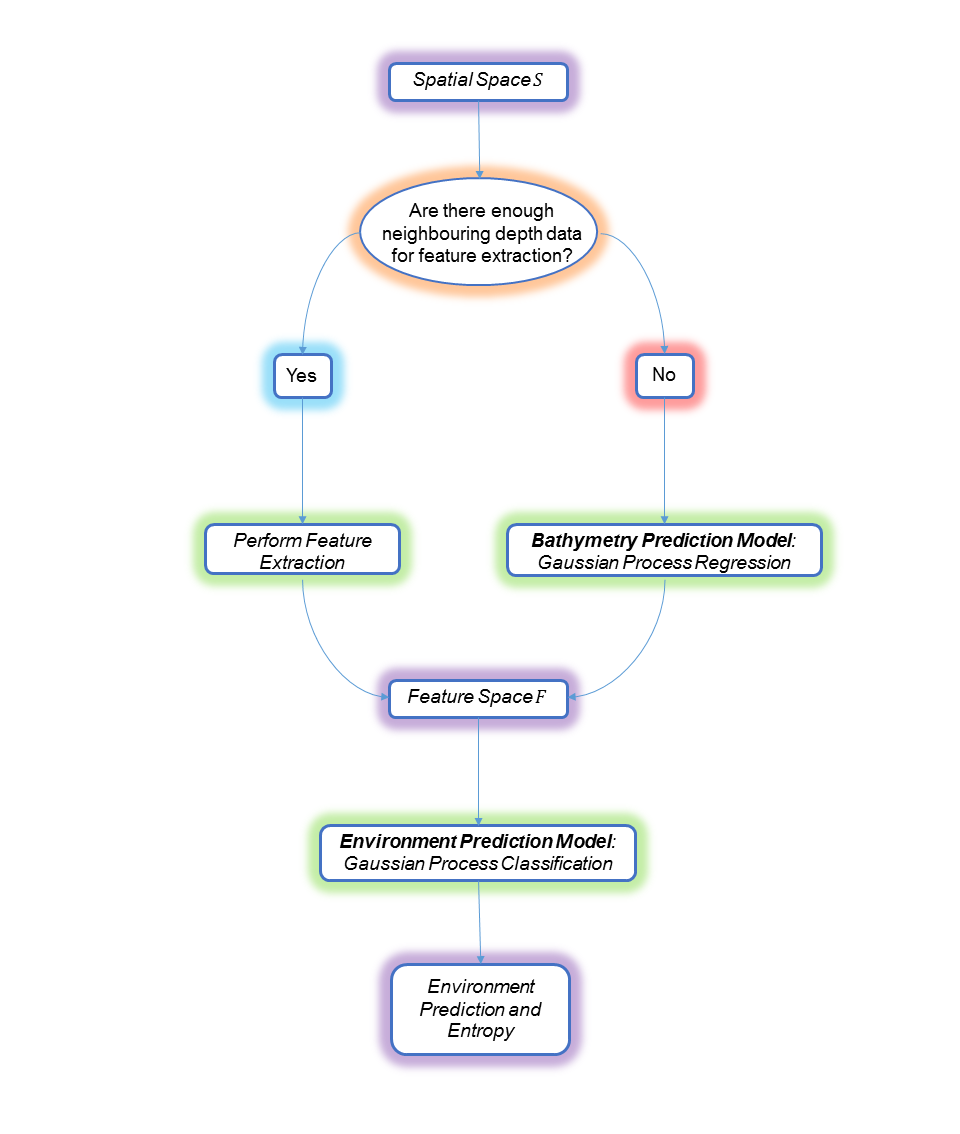
\includegraphics[width=\textwidth]{Figures/modelingprocess.png}
			\caption{Environment Modeling}
			\label{Background:OceanEnvironmentModeling:Figure:modelingprocess}
		\end{figure}
				
		In that case, a Gaussian process regression model is proposed for predicting the features at a given spatial location. While this is much more computationally expensive than performing feature extraction, it is also quite rare that this is necessary under abundant bathymetric data.
		
		Finally, once the feature vectors are obtained at training locations, the environment type is to be predicted. The environment type is summarised through labels that indicate the type of marine environment that was observed or predicted. Common AUV mission examples include "reef", "sand", and "rocks". These labels are often summarised through processing visual and stereo imagery obtained through past AUV missions. With a discrete set of possible labels, the environment prediction problem is to be modeled as a Gaussian process classification problem. From here on, the environment prediction problem is understood to refer to the two stage process of feature extraction or modeling and environment label prediction, with the latter being the main bottleneck for this process.
		
		\FloatBarrier
		
		\subsection{Environment Modeling - Data Matching}
		\label{Background:OceanEnvironmentModeling:DataMatching}
		
			A subtlety that arises from the above formulation is that during the training stage, the bathymetric data and the label data are not necessarily observed at the same places. Figure \ref{Background:OceanEnvironmentModeling:Figure:illustrationBathymetricAgainstLabels} illustrates the spatial distribution of the two datasets in a typical setting.
		
			\begin{figure}[!htbp]
				\centering
					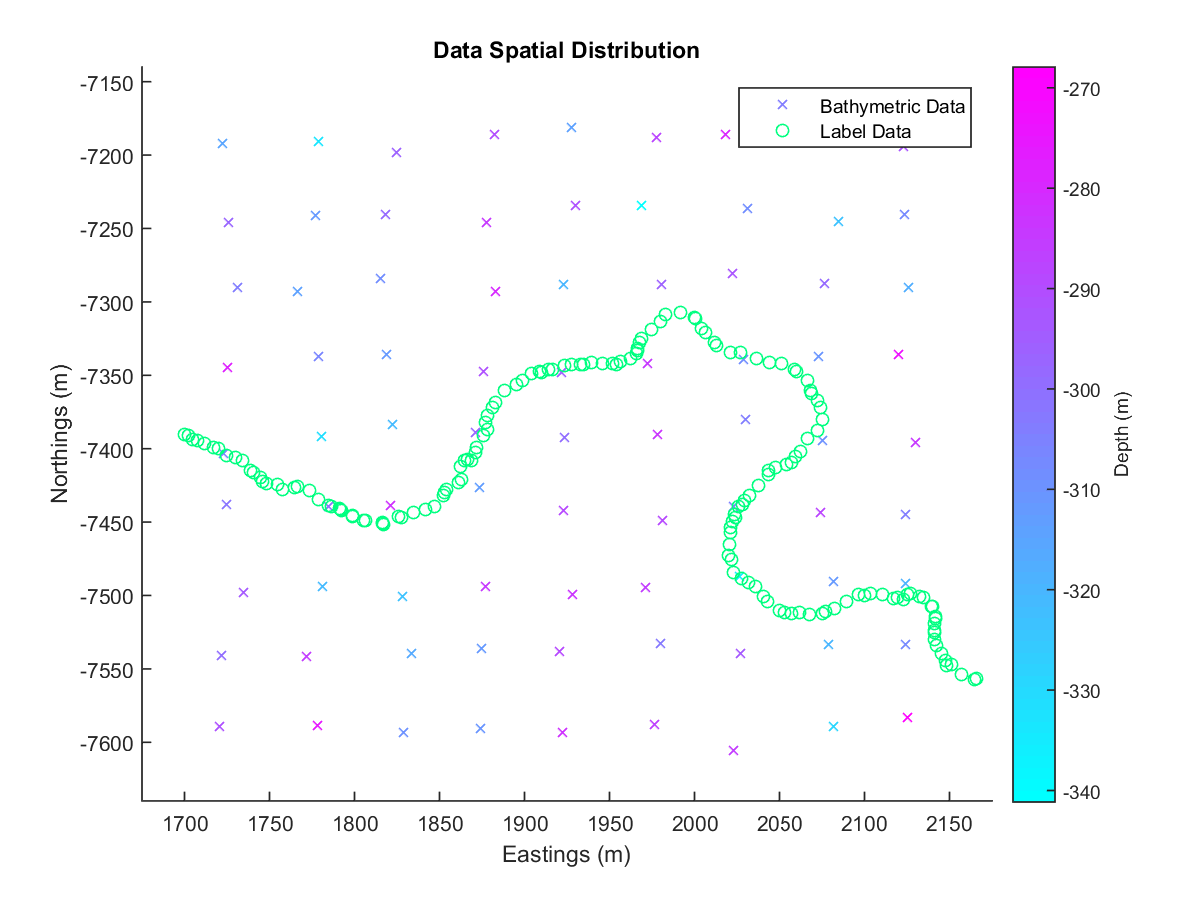
\includegraphics[width=0.9\textwidth]{Figures/illustrationBathymetricAgainstLabels.png}
				\caption{Illustration of Bathymetric and Label Data Density}
				\label{Background:OceanEnvironmentModeling:Figure:illustrationBathymetricAgainstLabels}
			\end{figure}
			
			While bathymetric data are usually collected rather uniformly, the label data are collected from past AUV missions whose trajectory are continuous curves across the ocean floor \citep{Squidle}. Due to slower AUV velocity as compared to surface ships which often employ SONAR or LIDAR techniques for bathymetry mapping, the label data are also spatially denser and concentrated on the mission trajectory, while being almost non-existent elsewhere.
			
			Therefore, in order to predict label data, the training data would need to be matched accurately. There are two straight forward choices at hand. The first is to estimate the bathymetric features at places where label data exists. However, at places near past mission paths, bathymetric data appears much more sparsely than label data, so that the feature extraction or regression prediction will yield very similar features across manly label data points. This reduces prediction power through a slow varying and limited feature group.
			
			Instead, the second choice is to estimate the label data at places where bathymetric data exists. In this setting, regions closer to past mission paths have higher volumes of label data, increasing the amount of training points. Regions further away would naturally generate more prediction uncertainty in the prediction stage.
			
			Hence, second method is chosen to be employed for data matching, in order to form our training set. Naturally, to predict environment labels from bathymetric features, we again need the Gaussian process classification model.
			
			\FloatBarrier
	
		\subsection{Feature Extraction}
		\label{Background:OceanEnvironmentModeling:FeatureExtraction}
		
			The feature extraction process assumes that the bathymetric depth data is available in grid form. That is, one can represent the available depth data $H = \{h_{k}\}_{k \in {1, 2, ..., N}}$ as $H = \{h_{ij}\}_{i \in {1, 2, ..., n_{i}}, \;\; j \in {1, 2, ..., n_{j}}}$ where varying $i$ and $j$ corresponds to varying data points in axis 1 and 2 respectively. Axis 1 and 2 is required to form an orthonormal frame. While axis 1 and 2 is usually aligned with the eastings-northings frame, it is generally not required for the feature extraction process.
			
			Without loss of generality, let $x$ and $y$ denote quantities corresponding to the orthogonal axes. We have that at $(x_{i}, y_{j})$ $(i \in {1, 2, ..., n_{i}}, \;\; j \in {1, 2, ..., n_{j}})$ the depth is measured as $h_{ij}$. The partial derivatives of various degrees of accuracy and scale can then be estimated through central differencing, as shown in \cref{Background:OceanEnvironmentModeling:Figure:centraldifferencecofficients} \citep{CentralDifferenceTable}. The author has chosen $N = 3$ neighbors for short scale slope and $N = 9$ neighbors for large scale slope.
			
			\begin{figure}[!htbp]
				\centering
					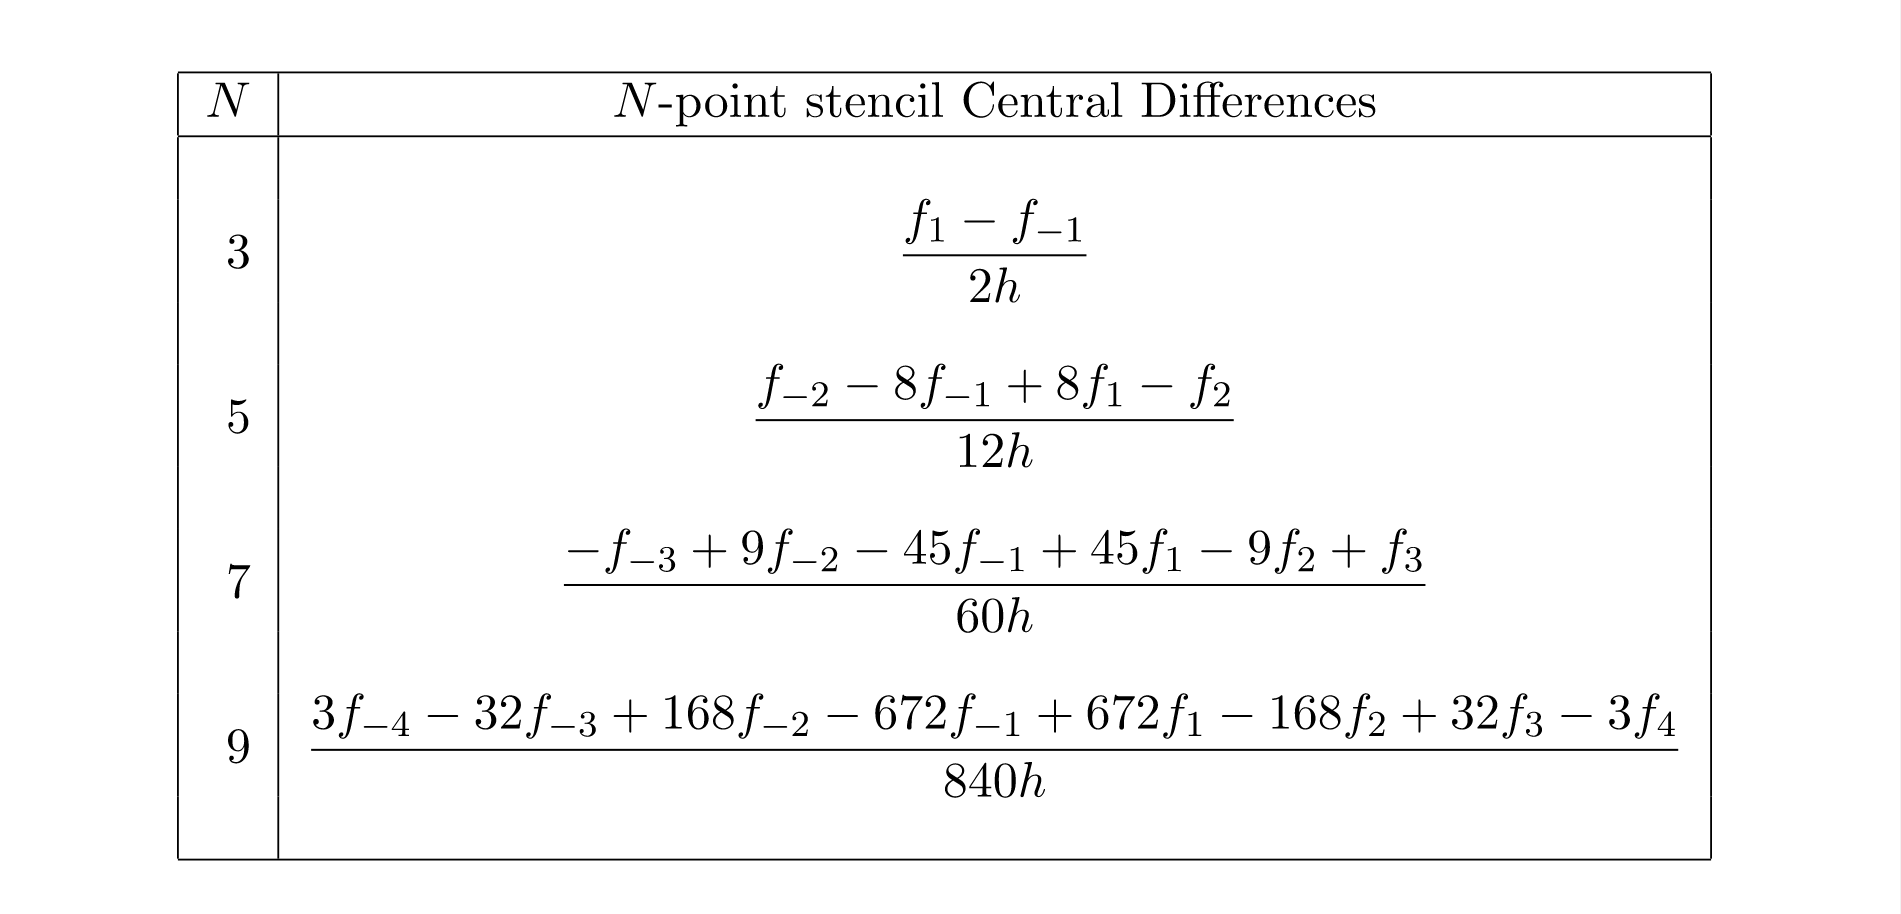
\includegraphics[width=0.9\textwidth]{Figures/centraldifferencecofficients.png}
				\caption{Finite Difference Methods: Central Difference Coefficients \\
				The subscripts $i$ represents  }
				\label{Background:OceanEnvironmentModeling:Figure:centraldifferencecofficients}
			\end{figure}			

			Central differencing is chosen as it is more numerically accurate. The disadvantages of instability and slightly higher time complexity from dynamic cases are not present in the static feature extraction process. Nevertheless, forward differencing is to be used at the boundaries of the dataset where neighboring data is missing on one side.
						
			With two axis, the result is a 2 element gradient vector. It is possible to treat the 2 elements as separate features. However, this would make the modeling problem frame dependent unnecessarily. Therefore, the magnitude of this gradient vector is taken as the slope feature. 
			
			Rugosity is a measure of local height variations in the terrain. By definition, its form is computed as $r = A_{r}/A_{g}$, the real surface area divided by the geometric surface area.
			
			Under cases without perfect grid formation, such as that shown in \cref{Background:OceanEnvironmentModeling:Figure:illustrationBathymetricAgainstLabels}, this feature extraction process becomes only an approximation. As the data set deviates from the form assumed above, it can then become necessary to estimate the features using Gaussian process regression - specifically, the multi-task Gaussian process regression. 
			
		 	On the other hand, under fine-scale bathymetric reconstructions, more sophisticated methods for deriving multi-scale measures of rugosity and slope exist. For example, under bathymetry measurements that are geo-referenced through stereo imagery, rugosity can be calculated through a Delaunay triangulated surface mesh and projecting areas onto the plane of best fit using Principal Component Analysis (PCA) \citep{StefanWilliams:Rugosity}.
							
			\FloatBarrier
				
	\section{Modeling on Test Data Sets}
	
	\section{Comparison: Laplace Approximation and Probabilistic Least Squares}
	
		Compare probability outputs, classification outputs, entropy outputs, etc
	
	\section{Comparison: OVA and AVA methods for multiclass classifiers}
	
	\section{Comparison: Probability fusion methods for multiclass classifiers}
	
%		\subsection{Normalisation Method}
%			
%		\subsection{Mode Keeping}
%			
%		\subsection{Exclusion}
			
	\section{Modeling the Scott Reef Environment}
	
		\subsection{Problems and Solutions to Big Data Analysis}
		
		\subsection{Feature Extraction}
		
		\subsection{Case with 4 Labels}
		
			(With different amounts of sampled points)
			
		\subsection{Case with 17 Labels}
		
	\section{Measuring Mutual Information}
	
		\subsection{Motivation}
			For both modeling purposes and path planning purposes, simply knowing the entropy at each query point is not enough. 
			
		\subsection{Shannon Entropy}
		
		\subsection{Lack of a Closed Form Solution}
		
	\section{A Direct Approach: Monte Carlo Sampling}
		
		\subsection{Development of Methodology}
		
			Provide pseudocode for limited and good way of doing it
			
		\subsection{Binary Classification}
		
		\subsection{Multi-class Classification}
		
	\section{A Faster Approach: Linearised Entropy}
		
		\subsection{Development of Methodology}
		
		\subsection{Binary Classification}
		
			For binary classification, linearisation is performed on the sigmoid, or response, function.
		
			The queried latent vector $\vec{f}$, a finite collection of latent function instances at query points, are distributed as a multivariate Gaussian distribution which can be computed from (equation). 
			
			\begin{equation}
				\vec{f} = [f_{1}, f_{2}, \dots, f_{n_{q}}]^{T} \sim \mathcal{N}(\vec{\mu}, \Sigma)
			\end{equation}
				
			\begin{equation}
				\pi_{i} = \sigma(f_{i}) \qquad \qquad \forall i \in I_{\mathrm{query}} = {1, 2, \dots, n_{q}}
			\end{equation}
			
		\subsection{Multi-class Classification}
		
			For multi-class classification, linearisation is performed on the softmax function for each class.
			
			Provide intuitive reason for the squashing.
			
		

\chapter{Informative Seafloor Exploration}
\lhead{Informative Seafloor Exploration}
\label{InformativeSeafloorExploration}

	The Gaussian process based inference model for benthic habitat mapping devised in Chapter \ref{BenthicHabitatMapping} provides a Bayesian framework for habitat inference and prediction. With such an inference model, this chapter proceeds to develop an informative path planning policy for benthic habitat mapping.
	
	In order to devise an informative path planning policy, it is important to select an appropriate acquisition criterion which measures the desirability of traversing a particular candidate path. Section \ref{Background:RelatedWork} provided an outline of related investigations on various acquisition functions for informative path planning in the benthic habitat mapping context, which motivated the need for a measure of mutual information. Such a measure would allow inference based on the \textit{essential} information contained in any given sub-region of interest. The mutual information criterion can then be employed as the acquisition function for informative path planning, in order to evaluate and thus compare the desirability of visiting candidate regions and locations.
	
	Nevertheless, as Gaussian process classifiers lack analytical forms for the \textit{predictive} joint distribution of target labels, any mutual information measure derived from the predictive joint distribution must rely on numerical estimation techniques. As such, estimating joint prediction information entropy requires a Monte Carlo sampling based approach. Section \ref{InformativeSeafloorExploration:MCPIE} describes such a mutual information criterion, hereby named Monte Carlo Predictive Information Entropy (MCPIE).
	
	However, a Monte Carlo approach suffers some several drawbacks, such as computational complexity and limited estimation accuracy. Instead, this thesis proposes a new and alternative mutual information measure, Linearised Model Differential Entropy (LMDE), that is more computationally tractable than MCPIE. Instead of focusing on the \textit{predictive} joint distribution, LMDE focuses on utilising the \textit{latent} joint distribution, where inference remains analytically tractable. Section \ref{InformativeSeafloorExploration:LMDE} defines and derives LMDE as an appropriate form of mutual information. Specifically, it regularises between reducing mutual bias and mutual uncertainty through taking advantage of both the latent mean and covariance structure, as well as the non-Gaussian likelihood response. Tractability of the approach is further improved through a linearisation approximation on such an acquisition criterion.
	
	Section \ref{InformativeSeafloorExploration:ComparisonMutualEntropyMeasures} proceeds to demonstrate the two mutual entropy measures through example datasets. Interpretation of the experimental results provides an intuitive understanding of their differences in time complexity, accuracy, and most importantly, their properties.
	
	Section \ref{InformativeSeafloorExploration:RecedingHorizonFormulation} then formulates a receding horizon approach to informative path planning. This provides a simple yet effective framework for a large scale exploration task such as seafloor exploration for benthic habitat mapping. In particular, the receding horizon formulation strikes a balance between exploring in a non-myopic way and doing so with reasonable tractability constraints.
	
	Finally, Section \ref{InformativeSeafloorExploration:ScottReef} assesses the performance of various approaches to informative seafloor exploration for benthic habitat mapping. Multiple acquisition criterions are tested under both the receding horizon approach and a myopic greedy approach, which verifies the benefits of linearised model differential entropy under the receding horizon formulation. Under a mapping accuracy criterion, simulations over the Scott Reef dataset demonstrates that LMDE acquisition outperform other criterions, including MCPIE acquisition.
		
	\section{Monte Carlo Predictive Information Entropy}
	\label{InformativeSeafloorExploration:MCPIE}
	
		This section introduces the Monte Carlo predictive information entropy (MCPIE) of Gaussian process classifiers. Monte Carlo sampling methods provide a way to estimate the joint predictive entropy through considering the joint distributions of the latent function at the query points.
	
		Monte Carlo sampling, as its name suggests, involve using sampled draws from a particular distribution to estimate a certain quantity that can be characterised by the distribution. In MCPIE case, the distribution to be sampled from is the latent GP process of the GP classifier, whose moments are analytically tractable, and the quantity to be estimated is the \textit{joint} predictive information entropy of the query points. A brief description of the method is provided for both binary and multiclass classification.
		
		\subsection{Binary Classification}
		\label{InformativeSeafloorExploration:MCPIE:Binary}
		
			Suppose a Gaussian process classifier has been trained under Laplace approximation with respect to a training set $\mathcal{D} = \{X, \bvec{y}\} = \{[ \bvec{x}_{1}, \bvec{x}_{2}, \dots, \bvec{x}_{n}]^{T}, [y_{1}, y_{2}, \dots, y_{n}]^{T}\}$ with $n$ training points. It is known that the latent function $f(\bvec{x})$ is distributed as a GP with a particular predictive mean $m(\bvec{x})$ and covariance $k(\bvec{x}, \bvec{x}')$ once conditioned on the training data \eqref{Equation:PredictiveLatentBinaryGP}. Note that again this chapter will omit explicitly notating the training data and query data that was conditioned upon, as well as the learned hyperparameters $\vec{\uptheta}$, unless otherwise stated. \begin{equation}
				f(\bvec{x}) \sim \mathcal{GP}(m(\bvec{x}), k(\bvec{x}, \bvec{x}'))
			\label{Equation:PredictiveLatentBinaryGP}
			\end{equation}
			
			Let $X^{\star} = [ \bvec{x}^{\star}_{1}, \bvec{x}^{\star}_{2}, \dots, \bvec{x}^{\star}_{n^{\star}}]^{T}$ denote the collection of $n^{\star}$ query points for which inference is to be performed upon. Denote $\bvec{f}^{\star}$ the vector of latent function values $f^{\star}_{i} = f(\bvec{x}^{\star}_{i})$ at each query point. By definition of a GP, $\bvec{f}^{\star}$ is multivariate Gaussian distributed with corresponding means $\mu^{\star}_{i} = m(\bvec{x}^{\star}_{i})$ and covariances $\Sigma^{\star}_{ij} = k(\bvec{x}^{\star}_{i}, \bvec{x}^{\star}_{j})$ \eqref{Equation:BinaryPredictiveGaussianDistribution}. \begin{equation}
				\bvec{f}^{\star} = [f^{\star}_{1}, f^{\star}_{2}, \dots, f^{\star}_{n^{\star}}]^{T} \sim \mathcal{N}(\vec{\upmu}^{\star}, \Sigma^{\star})
			\label{Equation:BinaryPredictiveGaussianDistribution}
			\end{equation}
				
			The binary prediction probability $\vec{\uppi^{\star}}$ at the query points is obtained through passing the queried latent function random vector $\bvec{f}^{\star}$ through a response function in a component wise fashion \eqref{Equation:PredictiveResponse}. \begin{equation}
				\vec{\uppi}^{\star} = \vec{\upsigma}(\bvec{f}^{\star})\mathrm{ \quad i.e. \;\;}\pi^{\star}_{i} = \sigma(f^{\star}_{i}) \quad \forall i \in I_{n^{\star}}
			\label{Equation:PredictiveResponse}
			\end{equation}
			
			As a straightforward transformation of the latent vector, the predictive probability vector $\vec{\uppi^{\star}}$ is thus a random vector itself. The usual procedure is then to treat the expected prediction probabilities $\mathbb{E}[\vec{\uppi^{\star}}]$ as the posterior class probabilities for further inference. However, this discards any information regarding the joint behaviour of an arbitrary collection of query points. As a result, a measure of mutual information shared amongst the query points cannot be obtained.
			
			As such, one straightforward approach to address this problem is to perform Monte Carlo estimation of the posterior joint distribution for class predictions via jointly sampling latent vectors from the GP latent, whose distribution is completely characterised through \eqref{Equation:PredictiveLatentBinaryGP} and definition \ref{Definition:GaussianRandomField}. For each jointly sampled vector, the components with positive latent values are assigned class label 1, and -1 otherwise. That is, for a particular sample ${^{s}}\bvec{f}^{\star}$ drawn from $\bvec{f}^{\star} \sim \mathcal{N}(\vec{\upmu}^{\star}, \Sigma^{\star})$ \eqref{Equation:BinaryPredictiveGaussianDistribution}, $s \in I_{n_{S}}$ where $n_{S}$ is the number of samples, the corresponding class assignments are computed through \eqref{Equation:MonteCarloSamplingBinaryClassifier}. Here, the left superscript $s$ indexes the sampled value or vector. As before, without the left superscript $s$, $\bvec{f}^{\star}$ is a random vector, while ${^{s}}\bvec{f}^{\star}$ is a particular realised, fixed vector. \begin{equation}
				{^{s}}\bvec{y}^{\star} = \bvec{\mathds{H}}({^{s}}\bvec{f}^{\star}) := \{\mathbb{H}({^{s}}f^{\star}_{i})\}_{i \in I_{n^{\star}}} \quad \forall s \in I_{n_{s}} \quad \mathrm{where} \quad \mathbb{H}(z) := \mathds{1}_{\{z > 0\}} - \mathds{1}_{\{z \leq 0\}}
			\label{Equation:MonteCarloSamplingBinaryClassifier}
			\end{equation}
			
			where $\mathbb{H}(z)$ is the modified Heaviside function which is 1 is $z$ is positive and -1 otherwise, so that ${^{s}}\bvec{y}^{\star} \in \{-1, 1\}^{n_{S}}$. Note that the sampled labels can be determined completely from the sampled latent function as, once sampled, the latent function is no longer a random function. Hence, any positive (negative) latent values will map to prediction probabilities of more (less) than 0.5 under any likelihood response.
			
			Further, define $I_{U} \subseteq I_{n_{S}}$, $n_{U} := \Vert I_{U} \Vert$, as the indices corresponding to the subset with the maximum amount of unique samples \eqref{Equation:UniqueIndexSet}, where $\Vert I \Vert$  stands for the cardinality of $I$. An \textit{estimated} probability vector $\tilde{\bvec{p}}$ can then be formed \eqref{Equation:EstimatedProbability}. \begin{equation}
				I_{U} := \argmax_{\{I \subseteq I_{n_{S}} | {^{s}}\bvec{y}^{\star} \neq {^{t}}\bvec{y}^{\star}, \forall s, t \in I\}} \Vert I \Vert 
			\label{Equation:UniqueIndexSet}
			\end{equation} \begin{equation}
				\begin{aligned}
					\tilde{\bvec{p}}^{\star} &:= \bigg\{ \frac{1}{n_{S}}\mathbb{F}_{I_{n_{S}}}({^{s}}\bvec{y}^{\star}) \bigg\}_{s \in I_{U}} \\
					\mathbb{F}_{I_{n_{S}}}({^{s}}\bvec{y}^{\star}) &:= \sum_{t \in I_{n_{S}}} \mathds{1}_{\{{^{s}}\bvec{y}^{\star} = {^{t}}\bvec{y}^{\star}\}}
				\end{aligned}
			\label{Equation:EstimatedProbability}
			\end{equation}
			
			where $\mathbb{F}_{I_{n_{S}}}({^{s}}\bvec{y}^{\star})$ is the frequency of appearance of the vector ${^{s}}\bvec{y}^{\star}$ amongst all the sampled vectors $\{ {^{s}}\bvec{y}^{\star} \}_{s \in I_{n_{S}}}$. Note that each \textit{unique} sample is assigned a probability such that the vector $\tilde{\bvec{p}}^{\star}$ has exactly $n_{U}$ non-zero entries indexed by $I_{U}$, which is generally smaller than the total number of possible samples. This inherently means that possible samples that were not drawn or \textit{realised} are estimated with probability zero. In this way, since more samples would likely realise those unlikely possibilities and thus raising the corresponding probability to a nonzero value, estimation accuracy will benefit from higher numbers of samples $n_{S}$.
			
			Finally,  for $n_{C} = 2$ classes, the Monte Carlo predictive information entropy, as an instance of Shannon entropy \eqref{Equation:DiscreteEntropy}, can be computed from the estimated probabilities that represent the joint distribution \eqref{Equation:MCPIE}. As usual, only non-zero entries of $\tilde{\bvec{p}}$ need to be considered. \begin{equation}
				H_{\mathrm{MCPIE}} \stackrel{\text{abbrev.}}{:=} H_{\mathrm{MCPIE}}[X^{\star} | X, \bvec{y}] := - \sum_{i \in I_{n_{U}}} \tilde{p}^{\star}_{i} \log(\tilde{p}^{\star}_{i})
			\label{Equation:MCPIE}
			\end{equation}		
			
		\subsection{Multiclass Classification}
		\label{InformativeSeafloorExploration:MCPIE:Multiclass}
		
			The derivation in the multiclass case is similar to the binary case. Specifically, since ${^{s}}\bvec{y}^{\star} \in \{1, 2, \dots, n_{C}\}^{n_{s}}$ it suffices to replace the sampling step \eqref{Equation:MonteCarloSamplingBinaryClassifier} with \eqref{Equation:MonteCarloSamplingMulticlassClassifierOVA} in the OVA case or \eqref{Equation:MonteCarloSamplingMulticlassClassifierAVA} in the AVA case, and apply \eqref{Equation:UniqueIndexSet}, \eqref{Equation:EstimatedProbability}, and \eqref{Equation:MCPIE} as before.
			
			The technique is first developed for an OVA multiclass classifier (see Section \ref{BenthicHabitatMapping:Classification:MulticlassClassification:OVA}), and then for an AVA multiclass classifier (see Section \ref{BenthicHabitatMapping:Classification:MulticlassClassification:AVA}) through reducing the AVA form into an OVA form. 
			
			\subsubsection{One Versus All Classifier}
			\label{InformativeSeafloorExploration:MCPIE:Multiclass:OVA}
			
				Analogous to \eqref{Equation:PredictiveLatentBinaryGP}, for $c$ classes, there are $n_{C}$ latent functions $\{f^{1}(x), f^{2}(x), \dots, f^{n_{C}}(x)\}$ corresponding to each class \eqref{Equation:PredictiveLatentMulticlassOVA}. \begin{equation}
					f^{c}(\bvec{x}) \sim \mathcal{GP}(m^{c}(\bvec{x}), k^{c}(\bvec{x}, \bvec{x}')) \qquad \forall c \in I_{n_{C}}
				\label{Equation:PredictiveLatentMulticlassOVA}
				\end{equation}
							
				Here the superscript $c$ is used to index the classes. The latent vector $\bvec{f}_{i} := \{f^{c}_{i}\}_{c \in I_{n_{C}}}$ represents the collection of $n_{C}$ latent values across classes at the query point $i \in I_{n^{\star}}$, and is distinct from $\bvec{f}^{c} := \{f^{c}_{i}\}_{i \in I_{n^{\star}}}$ which represents the collection of $n^{\star}$ latent values across query points for class $c \in I_{n_{C}}$.
				
				Again, by definition of a GP, each ${\bvec{f}^{c}}^{\star}$ is multivariate Gaussian distributed with corresponding means ${\mu^{c}}^{\star}_{i} = m^{c}(\bvec{x}^{\star}_{i})$ and covariances ${\Sigma^{c}}^{\star}_{ij} = k^{c}(\bvec{x}^{\star}_{i}, \bvec{x}^{\star}_{j})$ \eqref{Equation:MulticlassPredictiveGaussianDistributionOVA}. \begin{equation}
					{\bvec{f}^{c}}^{\star} = [{f^{c}_{1}}^{\star}, {f^{c}_{2}}^{\star}, \dots, {f^{c}_{n^{\star}}}^{\star}]^{T} \sim \mathcal{N}({\vec{\upmu}^{c}}^{\star}, {\Sigma^{c}}^{\star})
				\label{Equation:MulticlassPredictiveGaussianDistributionOVA}
				\end{equation}
				
				For each class $c$, a sample ${^{s}}{\bvec{f}^{c}}^{\star}$ is drawn from ${\bvec{f}^{c}}^{\star} \sim \mathcal{N}({\vec{\upmu}^{c}}^{\star}, {\Sigma^{c}}^{\star})$, where $s \in I_{n_{S}}$. The corresponding sampled target labels are then found by \eqref{Equation:MonteCarloSamplingMulticlassClassifierOVA}. \begin{equation}
					\begin{aligned}
						{^{s}}\bvec{y}^{\star} = \bvec{\mathds{M}}_{n_{C}}({^{s}}{\bvec{f}^{1}}^{\star}, {^{s}}{\bvec{f}^{2}}^{\star}, \dots, {^{s}}{\bvec{f}^{n_{C}}}^{\star}) &:= \{\mathbb{M}_{n_{C}}({^{s}}{f^{1}_{i}}^{\star}, {^{s}}{f^{2}_{i}}^{\star}, \dots, {^{s}}{f^{n_{C}}_{i}}^{\star})\}_{i \in I_{n^{\star}}} \quad \forall s \in I_{n_{s}} \\
						\mathrm{where} \qquad \mathbb{M}_{n_{C}}(z_{1}, z_{2}, \dots, z_{n_{C}}) &:= \argmax_{c \in I_{n_{C}}} z_{c}
					\end{aligned}
				\label{Equation:MonteCarloSamplingMulticlassClassifierOVA}
				\end{equation}
				
				That is, for each sample $s \in I_{n_{S}}$ and at each query point $i \in I_{n^{\star}}$, ${^{s}}y^{\star}_{i}$ is assigned the class label from $\{1, 2, \dots, n_{C}\}$ that has the maximal latent value. With the samples $\{{^{s}}\bvec{y}^{\star}\}_{s \in I_{n_{s}}}$, the estimated probability can be computed from \eqref{Equation:EstimatedProbability}, so that the Monte Carlo predictive information entropy for $n_{C} > 2$ classes in the OVA case can be computed from \eqref{Equation:UniqueIndexSet}, \eqref{Equation:EstimatedProbability}, and \eqref{Equation:MCPIE} as before.
			
			\subsubsection{All Versus All Classifier}
			\label{InformativeSeafloorExploration:MCPIE:Multiclass:All}
			
				For the AVA case, there are ${n_{C} \choose 2} = \frac{n_{C} (n_{C} - 1)}{2}$ latent functions $\{f^{1, 2}(x), f^{1, 3}(x), \dots, \\ f^{1, n_{C}}(x), f^{2, 3}(x), f^{2, 4}(x), \dots, f^{2, n_{C}}(x), \dots, f^{n_{C} - 1, n_{C}}(x)\}$ corresponding to class pairs $(c, c')$ with $c' > c$ \eqref{Equation:PredictiveLatentMulticlassAVA}. \begin{equation}
					f^{c, c'}(\bvec{x}) \sim \mathcal{GP}(m^{c, c'}(\bvec{x}), k^{c, c'}(\bvec{x}, \bvec{x}')) \qquad \forall c \in I_{n_{C}}, \quad c' \in \{c + 1, n_{C}\}
				\label{Equation:PredictiveLatentMulticlassAVA}
				\end{equation}
			
				Similarly, by definition of a GP, each ${\bvec{f}^{c, c'}}^{\star}$ is multivariate Gaussian distributed with corresponding means ${\mu^{c, c'}}^{\star}_{i} = m^{c, c'}(\bvec{x}^{\star}_{i})$ and covariances ${\Sigma^{c, c'}}^{\star}_{ij} = k^{c, c'}(\bvec{x}^{\star}_{i}, \bvec{x}^{\star}_{j})$ \eqref{Equation:MulticlassPredictiveGaussianDistributionAVA}. \begin{equation}
					{\bvec{f}^{c, c'}}^{\star} = [{f^{c, c'}_{1}}^{\star}, {f^{c, c'}_{2}}^{\star}, \dots, {f^{c, c'}_{n^{\star}}}^{\star}]^{T} \sim \mathcal{N}({\vec{\upmu}^{c, c'}}^{\star}, {\Sigma^{c, c'}}^{\star})
				\label{Equation:MulticlassPredictiveGaussianDistributionAVA}
				\end{equation}
				
				For each class pair $(c, c')$, a sample ${^{s}}{\bvec{f}^{c, c'}}^{\star}$ is drawn from ${\bvec{f}^{c, c'}}^{\star} \sim \mathcal{N}({\vec{\upmu}^{c, c'}}^{\star}, {\Sigma^{c, c'}}^{\star})$, where $s \in I_{n_{S}}$. Similar to filling the lower triangular region of \eqref{Equation:UnfilledProbabilityListAVA} through \ref{Equation:ProbabilityListAVA}, the above samples form the upper triangular parts of a double axis list, and the lower triangular region can be filled by setting ${^{s}}{\bvec{f}^{c', c}}^{\star} := -{^{s}}{\bvec{f}^{c, c'}}^{\star}$ by symmetry of binary classifiers \ref{Equation:SampleLatentListAVA}. Here, $\bvec{0}_{n^{\star}} := \{0\}_{i \in I_{n^{\star}}}$ is the zero vector, which represents the zero prior for the latent GP when no comparisons are to be made.
				
				\begin{equation}
					\begin{Bmatrix*}
						\bvec{0}_{n^{\star}} & {^{s}}{\bvec{f}^{1, 2}}^{\star} & {^{s}}{\bvec{f}^{1, 3}}^{\star} & \dots & {^{s}}{\bvec{f}^{1, n_{C}}}^{\star} \\
						{^{s}}{\bvec{f}^{2, 1}}^{\star} & \bvec{0}_{n^{\star}} & {^{s}}{\bvec{f}^{2, 3}}^{\star} & \dots & {^{s}}{\bvec{f}^{2, n_{C}}}^{\star} \\
						{^{s}}{\bvec{f}^{3, 1}}^{\star} & {^{s}}{\bvec{f}^{3, 2}}^{\star} & \bvec{0}_{n^{\star}} & \dots & {^{s}}{\bvec{f}^{3, n_{C}}}^{\star} \\
						\vdots & \vdots & \vdots & \ddots & \vdots \\
						{^{s}}{\bvec{f}^{n_{C}, 1}}^{\star} & {^{s}}{\bvec{f}^{n_{C}, 2}}^{\star} & {^{s}}{\bvec{f}^{n_{C}, 3}}^{\star} & \dots & \bvec{0}_{n^{\star}} 
					\end{Bmatrix*} \qquad \forall s \in I_{n_{S}}
				\label{Equation:SampleLatentListAVA}
				\end{equation}
				
				Again, each row corresponds to the ``strength'' of each class. A fair transformation into the OVA form can then be obtained by summing along the rows of the double axis list above for each sample $s \in I_{n_{S}}$. In this way, the corresponding sampled target labels are then found by the same way as the OVA case \eqref{Equation:MonteCarloSamplingMulticlassClassifierAVA}. Through this, the Monte Carlo predictive information entropy for $n_{C} > 2$ classes in the AVA case can also be computed from \eqref{Equation:UniqueIndexSet}, \eqref{Equation:EstimatedProbability}, and \eqref{Equation:MCPIE} as before. \begin{equation}
					\begin{aligned}
						{^{s}}{\bvec{f}^{c}}^{\star} :=& \sum_{c' = 1}^{n_{C}} {^{s}}{\bvec{f}^{c, c'}}^{\star} \qquad \text{where} \qquad {^{s}}{\bvec{f}^{c, c}}^{\star} := \bvec{0}_{n^{\star}} \qquad \forall c \in I_{n_{C}}, s \in I_{n_{S}} \\
						{^{s}}\bvec{y}^{\star} =& \quad \bvec{\mathds{M}}_{n_{C}}({^{s}}{\bvec{f}^{1}}^{\star}, {^{s}}{\bvec{f}^{2}}^{\star}, \dots, {^{s}}{\bvec{f}^{n_{C}}}^{\star}) \qquad \forall s \in I_{n_{s}}
					\end{aligned}
				\label{Equation:MonteCarloSamplingMulticlassClassifierAVA}
				\end{equation}
					
	\section{Linearised Model Differential Entropy}
	\label{InformativeSeafloorExploration:LMDE}
	
		This section introduces the linearised model differential entropy (LMDE) of Gaussian process classifiers. This information measure attempts to address the need for a measure of mutual entropy that is more computationally viable compared than Monte Carlo methods. Through investigating the structure of the GP classification inference model in both the binary and multiclass classification setting, a simple derivation for LMDE is provided.
		
		\subsection{Binary Classification}
		\label{InformativeSeafloorExploration:LMDE:Binary}
		
			For binary classification, linearisation is performed on the likelihood response.
					
			The beginning of this derivation is the same as Section \ref{InformativeSeafloorExploration:MCPIE:Binary} up to \eqref{Equation:PredictiveResponse}. At this stage, instead of proceeding with Monte Carlo sampling, it is proposed to use the joint distribution of the predictive probabilities $\vec{\uppi^{\star}}$ itself as a basis of constructing a measure of mutual information. Unlike traditional approaches where inference depends only on the expectance $\mathbb{E}[\vec{\uppi^{\star}}]$ and variance $\{\mathbb{V}[\pi^{\star}_{i}]\}_{i \in I_{n^{\star}}}$ such that structural information from the latent GP is compromised, it is aimed to utilise also the covariance $\mathbb{V}[\vec{\uppi^{\star}}]$, which contains information regarding both the latent GP and the response likelihood.
		
			\begin{figure}[!htbp]
				\centering
					\includegraphics[width = 0.6\linewidth]{Figures/linearisation.eps}
				\caption{Linearisation accuracy for a probit response: Green shade represents the latent variance while blue shade represents the predictive variance. Gold lines show local linearisation about latent expectance.}
				\label{Figure:Linearisation}
			\end{figure}
				
			As the predictive probabilities are nonlinear transformations of the Gaussian distributed latent vector, they are no longer Gaussian distributed. In order to retain analytical tractability, the proposed approach is to linearise the response function about the latent expectance $\bar{f}^{\star}_{i} := \mathbb{E}[f^{\star}_{i}]$. Figure \ref{Figure:Linearisation} illustrates the linearisation accuracy for a probit response. Observe that points with latent expectance far away from zero translate to near zero predictive variance even under high latent variance. Linearisation is thus very accurate for those points. For points with latent expectances near zero, we require the latent variances to be sufficiently small for linearisation to be accurate.
			
			The linearised can thus be derived, which also serves to construct the definition of linearised differential entropy. With first order Taylor expansion, the response is linearised the latent mean $\bar{f}^{\star}_{i} = \mathbb{E}[f^{\star}_{i}]$ \eqref{Equation:LinearisingSigmoid}. \begin{equation}
				\sigma(f^{\star}_{i}) \approx \sigma_{L}(f^{\star}_{i}) := \sigma(\bar{f}^{\star}_{i}) + \sigma'(\bar{f}^{\star}_{i}) (f^{\star}_{i} - \bar{f}^{\star}_{i})
			\label{Equation:LinearisingSigmoid}
			\end{equation}
			
			The prediction probabilities are now approximated as a linear transformation $\sigma_{L}(f)$ of the latent vector, so that it is also multivariate Gaussian distributed with expectance and covariance available in analytical form \eqref{Equation:MomentsLinearisedSigmoid}. \begin{align*}
			\numberthis \label{Equation:MomentsLinearisedSigmoid}
					\vec{\upsigma}_{L}(\bvec{f}^{\star}) & \sim \mathcal{N}(\vec{\upmu}^{\star}_{L}, \Sigma^{\star}_{L}) \\
					({\mu^{\star}_{L}})_{i} & = \mathbb{E}[\sigma_{L}(f^{\star}_{i})] = \sigma(\bar{f}^{\star}_{i}) \\
					({\Sigma^{\star}_{L}})_{ij} & = \mathbb{C}\mathrm{ov}[\sigma_{L}(f^{\star}_{i}), \sigma_{L}(f^{\star}_{j})] = \sigma'(\bar{f}^{\star}_{i}) \sigma'(\bar{f}^{\star}_{j}) \mathbb{C}\mathrm{ov}[f^{\star}_{i}, f^{\star}_{j}]
			\end{align*}
			
			Finally, the linearised model differential entropy $H_{\mathrm{LMDE}}$ at the query points $X^{\star}$ is defined to be the differential entropy corresponding to the random vector $\vec{\upsigma}_{L}(\bvec{f}^{\star})$. Since $\vec{\upsigma}_{L}(\bvec{f}^{\star})$ is multivariate Gaussian distributed, $H_{\mathrm{LMDE}}$ exhibits a closed form \eqref{Equation:BinaryLinearisedEntropy}. \begin{equation}
				H^{\mathrm{binary}}_{\mathrm{LMDE}} \stackrel{\text{abbrev.}}{:=} H^{\mathrm{binary}}_{\mathrm{LMDE}}[X^{\star} | X, \bvec{y}] := \frac{1}{2} \log\Big((2 \pi e)^{n^{\star}} \det(\Sigma^{\star}_{L})\Big)
			\label{Equation:BinaryLinearisedEntropy}
			\end{equation}			
						
		\subsection{Multiclass Classification}
		\label{InformativeSeafloorExploration:LMDE:Multiclass}
		
			For multiclass classification, linearisation is performed on the softmax function $\sigma^{c}$ which returns the corresponding predictive class probability $\vec{\uppi}^{c}$ for class $c \in I_{n_{C}} := \{1, 2, \dots, n_{C}\}$ \eqref{Equation:Softmax} \citep{GaussianProcessForMachineLearning}. \begin{equation}
				{\pi^{c}_{i}}^{\star} = \sigma^{c}({\bvec{f}_{i}}^{\star}) := \frac{\exp({f^{c}_{i}}^{\star})}{\sum_{m = 1}^{n_{C}} \exp({f^{m}_{i}}^{\star})} \qquad c \in I_{n_{C}}
			\label{Equation:Softmax}
			\end{equation}
			
			Similar to deriving the Monte Carlo prediction information entropy, the linearised model differential entropy is first derived in the OVA case. The treatment for the AVA case then again relies on transforming the AVA problem into an OVA problem so that the two share the bulk of the computations involved.
			
			\subsubsection{One versus All Classifier}
			\label{InformativeSeafloorExploration:LMDE:Multiclass:OVA}
			
				For $c$ classes, $c$ binary classifiers are trained independently and also performs inference independently. The normalisation is then inherently captured in the softmax \eqref{Equation:Softmax}. This approach avoids the Monte Carlo sampling step in the inference stage of a typical GP multiclass classifier under Laplace Approximation \citep{GaussianProcessForMachineLearning}, and is thus faster in computational time. Note that this Monte Carlo sampling step avoided is separate to the one used in MCJIE. In essence, using OVA classifiers skip one Monte Carlo step, and using LMDE skips another Monte Carlo step through avoiding using MCPIE. Furthermore, because each classifier is trained independently, both the learning stage and the inference stage can be performed in parallel, further speeding up the process in a way that was not available under the original scheme. This is important later in under a receding horizon formulation, where the inference stage is included in the objective function of an optimiser such that repeated evaluations would benefit dramatically from shorter inference time.
				
				Similar to the binary case, to linearise it is imperative to examine the gradient of each of the $c$ softmax functions \eqref{Equation:SoftmaxGradient}. For notational simplicity, the query stars ($^{\star}$) are omitted in this derivation except for $n^{\star}$. The numerators are explicitly left in the form of products of exponentiation instead of exponentiation of sums to reflect ways to cache quantities during computation. Hence, for each class $c$ at query point $i$ a softmax gradient vector is computed \eqref{Equation:SoftmaxGradientVector}. \begin{equation}
					\frac{\partial \sigma^{c}}{\partial f^{k}_{i}}(\bvec{f}_{i}) =
					\begin{cases} 
						- \frac{\exp(f^{c}_{i}) \exp(f^{k}_{i})}{\sum_{m = 1}^{n_{C}} \exp({f^{c}_{i}})} & \text{for } k \neq c  \\
						- \frac{\exp(f^{c}_{i})^{2}}{\big(\sum_{m = 1}^{n_{C}} \exp({f^{c}_{i}})\big)^{2}} + \frac{\exp(f^{c}_{i})}{\sum_{m = 1}^{n_{C}} \exp({f^{c}_{i}})}& \text{for } k = c
					\end{cases}
				\label{Equation:SoftmaxGradient}
				\end{equation} \begin{equation}
					\frac{\partial \sigma^{c}}{\partial \bvec{f}_{i}}(\bvec{f}_{i}) := \begin{bmatrix} \frac{\partial \sigma^{c}}{\partial f^{1}_{i}}(\bvec{f}_{i}) & \frac{\partial \sigma^{c}}{\partial f^{2}_{i}}(\bvec{f}_{i}) & \dots & \frac{\partial \sigma^{c}}{\partial f^{n_{C}}_{i}}(\bvec{f}_{i}) \end{bmatrix}^{T}
				\label{Equation:SoftmaxGradientVector}
				\end{equation} The linearisation is again performed on the mean latent predictions $\bar{\bvec{f}}_{i} = \mathbb{E}[\bvec{f}_{i}]$ so that each softmax $\sigma^{c}(\bvec{f}_{i})$ can be approximated with the linearised softmax $\sigma^{c}_{L}(\bvec{f}_{i})$ \eqref{Equation:LinearisedSoftmax} in an analogous form as \eqref{Equation:LinearisingSigmoid}, with the constants defined by $\bvec{a}^{c}_{i} := \sigma^{c}(\bar{\bvec{f}}_{i})$ and $\bvec{g}^{c}_{i} := \frac{\partial \sigma^{c}}{\partial \bvec{f}_{i}}(\bar{\bvec{f}}_{i})$. \begin{equation}
					\begin{aligned}
						\sigma^{c}(\bvec{f}_{i}) \approx \sigma^{c}_{L}(\bvec{f}_{i}) & := \sigma^{c}(\bar{\bvec{f}}_{i}) + \left. \frac{\partial \sigma^{c}}{\partial \bvec{f}_{i}} \right|^{T}_{\bvec{f}_{i} = \bar{\bvec{f}}_{i}} (\bvec{f}_{i} - \bar{\bvec{f}}_{i}) \\
						& = \bvec{a}^{c}_{i} + (\bvec{g}^{c}_{i})^{T} (\bvec{f}_{i} - \bar{\bvec{f}}_{i})
					\end{aligned}
				\label{Equation:LinearisedSoftmax}
				\end{equation} 
				
				To determine the distribution of the vector of softmax values across query points, first define the following \eqref{Equation:Definitions}. \begin{equation}
					\begin{aligned}
						F &:= \{f^{c}_{i}\}_{c \in I_{n_{C}}, i \in I_{n^{\star}}} \in \mathbb{R}^{n_{C} \times n^{\star}} \\
						\vec{\upsigma}^{c}_{L}(F) &:= \begin{bmatrix} \sigma^{c}_{L}(\bvec{f}_{1}) & \sigma^{c}_{L}(\bvec{f}_{2}) & \dots & \sigma^{c}_{L}(\bvec{f}_{n^{\star}}) \end{bmatrix}^{T} \qquad \forall c \in I_{n_{C}}
					\end{aligned}
				\label{Equation:Definitions}
				\end{equation} The covariance of the linearised softmax of a particular class $c$ between two query points $i$ and $j$ can now be computed, as well as the expectance at a particular query point $i$ \eqref{Equation:MomentsLinearisedSoftmax}. \begin{align*}
				\numberthis \label{Equation:MomentsLinearisedSoftmax}
						\vec{\upsigma}^{c}_{L}(F) & \sim \mathcal{N}(\vec{\upmu}^{c}_{L}, \Sigma^{c}_{L}) \\
						(\mu^{c}_{L})_{i} & = \mathbb{E}[\sigma^{c}_{L}(\bvec{f}_{i})] =  \sigma^{c}(\bar{\bvec{f}}_{i}) \\
						(\Sigma^{c}_{L})_{ij} & = \mathbb{C}\mathrm{ov}[\sigma^{c}_{L}(\bvec{f}_{i}), \sigma^{c}_{L}(\bvec{f}_{i})] \\
						& = \mathbb{C}\mathrm{ov}[(\bvec{g}^{c}_{i})^{T} \bvec{f}_{i}, (\bvec{g}^{c}_{j})^{T} \bvec{f}_{j}] \\
						& = \sum_{m = 1}^{n_{C}} (g^{c}_{i})^{m} (g^{c}_{j})^{m} \mathbb{C}\mathrm{ov}[f^{m}_{i}, f^{m}_{j}]
				\end{align*} where $(g^{c}_{i})^{m}$ denotes the $m^{\text{th}}$ element of $\bvec{g}^{c}_{i}$. The last equality arises as a result of employing OVA multiclass classification, where latent values of classes $c$ and $m$, $c \neq m$, are conditionally independent given training observations.
				
				Finally, the linearised model differential entropy of the OVA multiclass Gaussian process classifier is defined as follows \eqref{Equation:MulticlassLinearisedEntropy}. \begin{equation}
					H^{\mathrm{multiclass}}_{\mathrm{LMDE}} \stackrel{\text{abbrev.}}{:=} H^{\mathrm{multiclass}}_{\mathrm{LMDE}}[X^{\star} | X, \bvec{y}] := \frac{1}{2} \log\Bigg((2 \pi e)^{n^{\star}} \det\bigg(\sum_{c = 1}^{n_{C}} \Sigma^{c}_{L}\bigg)\Bigg)
				\label{Equation:MulticlassLinearisedEntropy}
				\end{equation}

			\subsubsection{All versus All Classifier}
			\label{InformativeSeafloorExploration:LMDE:Multiclass:AVA}
					
				Similar to the approach in the MCPIE derivation, the double axis list of latent vectors $\{ {\bvec{f}^{c, c'}}^{\star} \}_{c, c' \in I_{n_{C}}}$ where ${\bvec{f}^{c', c}}^{\star} = - {\bvec{f}^{c, c'}}^{\star}$ and ${\bvec{f}^{c, c}}^{\star} := \bvec{0}_{n^{\star}}$  are to be fused into $n_{C}$ latent vectors $\{ {\bvec{f}^{c}}^{\star} \}_{c \in I_{n_{C}}}$ through the same way as \eqref{Equation:MonteCarloSamplingMulticlassClassifierAVA} with ${\bvec{f}^{c}}^{\star} := \sum_{c' = 1}^{n_{C}} {\bvec{f}^{c, c'}}^{\star}$. However, here the latent vectors to be fused are now random vectors instead of fixed, sampled vectors as before. 
			
				As all of ${\bvec{f}^{c, c'}}^{\star}$ are multivarite Gaussian distributed, and are by construction independent after conditioning on their respectively hyperparameters $\vec{\uptheta}^{c, c'}$ which are not explicitly shown in notation here, the distribution of the fused latent vectors are given by \eqref{Equation:LatentFuseDistributionAVA}. These then provide the latent expectance vector and covariance matrix used in \eqref{Equation:MomentsLinearisedSoftmax}, from which the computations continues as in the OVA scheme. \begin{equation}
					\begin{aligned}
						\mathbb{E}[{\bvec{f}^{c}}^{\star}] := \sum_{c' = 1}^{n_{C}} \mathbb{E}[{\bvec{f}^{c, c'}}^{\star}] \qquad \qquad \mathbb{V}[{\bvec{f}^{c}}^{\star}] := \sum_{c' = 1}^{n_{C}} \mathbb{V}[{\bvec{f}^{c, c'}}^{\star}]
					\end{aligned}
				\label{Equation:LatentFuseDistributionAVA}
				\end{equation}
				

				
%				\begin{equation}
%					\begin{Bmatrix*}
%						\bvec{0}_{n^{\star}} & {\bvec{f}^{1, 2}}^{\star} & {\bvec{f}^{1, 3}}^{\star} & \dots & {\bvec{f}^{1, n_{C}}}^{\star} \\
%						{\bvec{f}^{2, 1}}^{\star} & \bvec{0}_{n^{\star}} & {\bvec{f}^{2, 3}}^{\star} & \dots & {\bvec{f}^{2, n_{C}}}^{\star} \\
%						{\bvec{f}^{3, 1}}^{\star} & {\bvec{f}^{3, 2}}^{\star} & \bvec{0}_{n^{\star}} & \dots & {\bvec{f}^{3, n_{C}}}^{\star} \\
%						\vdots & \vdots & \vdots & \ddots & \vdots \\
%						{\bvec{f}^{n_{C}, 1}}^{\star} & {\bvec{f}^{n_{C}, 2}}^{\star} & {\bvec{f}^{n_{C}, 3}}^{\star} & \dots & \bvec{0}_{n^{\star}}
%					\end{Bmatrix*} 
%				\label{Equation:LatentListAVA}
%				\end{equation}
			
	\section{Comparison of Mutual Entropy Measures}
	\label{InformativeSeafloorExploration:ComparisonMutualEntropyMeasures}
	
		Both Monte Carlo prediction information entropy and linearised model differential entropy are suitable measures of mutual entropy that can be used as an acquisition criterion for informative path planning. This section provides a simple comparison between the two entropy measures with example datasets, which would further assist in the interpretation of model differential entropy. The main takeaway is that MCPIE and LMDE are complementary measures of entropy which together captures uncertainty in prediction and uncertainty in the model respectively.
	
		\subsection{Estimation Accuracy under Monte Carlo Sampling}
		\label{InformativeSeafloorExploration:ComparisonMutualEntropyMeasures:EstimationAccuracy}
		
			It is helpful to visualise the practical numbers of samples required for reasonable estimation accuracy for MCPIE. Figure \ref{Figure:mcpie_lmde_comparison_binary} shows a simple case for a binary classification scenario. The training data is evenly distributed in the feature space with features $x_{1}$ and $x_{2}$, and the MCPIE is estimated with 2500 samples \textit{at each query point}. Note that only the marginalised entropies can visualised, as it is difficult to visualise multiple regional entropies. However, this is sufficient to provide an intuition for the accuracy of the method.
			
			\begin{figure}[!htbp]
				\centering
					\includegraphics[width = \linewidth]{Figures/mcpie_lmde_comparison_binary/mcpie_lmde_comparison.eps}
				\caption{GP binary classifier example}
				\label{Figure:mcpie_lmde_comparison_binary}
			\end{figure}			
					
			Since only the marginalised entropies are visualised, there exists analytical forms for prediction information entropy by computing the Shannon entropy over the expected prediction probabilities at each query point. For a multiclass case under the OVA formulation, the probabilities are fused using the \textit{exclusion} method (see section  \ref{BenthicHabitatMapping:Classification:Multiclass:ProbabilityFusion}). Subplots (2, 1) and (2, 2) of Figure \ref{Figure:mcpie_lmde_comparison_binary} show the analytically computed PIE and Monte Carlo estimated PIE (MCPIE) respectively, which shows that the estimation is fairly accurate with 2500 samples.
			
			\begin{figure}[!htbp]
				\centering
					\includegraphics[width = \linewidth]{Figures/mcpie_lmde_comparison_binary/mcpie_accuracy.eps}
				\caption{Accuracy improvement of MCPIE for a binary case}
				\label{Figure:mcpie_accuracy_binary}
			\end{figure}
				
			Figure \ref{Figure:mcpie_accuracy_binary} visualises the accuracy improvement as more samples are used for entropy estimation. With small samples, the estimation is noisy and inaccurate, and generally converges to a reasonable accuracy after 1000 samples. Notice however that even with low numbers of samples, the entropies are mostly in the correct range already. Appendix \ref{Appendix:MutualEntropyMeasures} provides the same results for the multiclass case.
			
		\subsection{Interpretation of Model Differential Entropy}
		\label{InformativeSeafloorExploration:ComparisonMutualEntropyMeasures:InterpretationMDE}
		
			It is worthwhile to remember that model differential entropy and its linearisation is not an approximation to the usual prediction information entropy - the former is a differential entropy on a multivariate Gaussian distribution and the latter is an information entropy on the distribution of discrete class predictions combinations, which is a multivariate multinomial distribution. They have different interpretations and both can have advantageous properties under different scenarios. It is proposed that using linearised model differential entropy as an alternative acquisition function for informative path planning can be more beneficial under specific exploration purposes.
			
			Specifically, while the prediction information entropy (PIE) represents the confidence in the model, the model differential entropy (MDE) represents the the separability of classes in the feature space. In fact, MDE quantifies the ambiguity of the predictive probabilities. In particular, it is possible for GP multiclass classifiers to conclude low predictive variance even under uncertain predictive probabilities. In this case, the MDE would be high while the PIE would be low at such locations, indicating that the model is confident about its inability to separate classes \citep{AsherBender}. Similar to the bias-variance trade-off, such a situation indicate high bias, and is distinct from a model that is unconfident about its ability to separate classes, which would correspond to high variance. In fact, as the entropy of the prediction probabilities, model differential entropy is so named as it measures the uncertainty in the model itself. While an uncertainty in the model propagates into uncertainty in the prediction, it also propagates into bias in the prediction as an inaccurate model is unlikely to predict the correct class labels on average. This demonstrates that PIE and MDE are two complementary measures of entropy that can assist each other in identifying both places of high bias and high variance.
			
			In this way, using MDE as the acquisition function means that the vehicle would prioritise on both getting the both the model and predictions as correct as possible, instead of only focusing on predictions as in the PIE case.
			
		\subsection{Advantage of Model Differential Entropy}
		\label{InformativeSeafloorExploration:ComparisonMutualEntropyMeasures:AdvantagesMDE}
		
			Here the examples from Figures \ref{Figure:mcpie_lmde_comparison_binary} and \ref{Figure:mcpie_lmde_comparison_multiclass} are discussed further in detail.
			
			With abundant and evenly distributed training data, the classifiers achieves a misclassification rate of only 2.2\% and 8.6\% respectively. The classifiers are trained with an axis aligned Gaussian kernel with a probit response under Laplace approximation. 
			
			Intuitively, under abundant data, it is desired that the classifier would only indicate high entropies at decision boundaries. In Figure \ref{Figure:mcpie_lmde_comparison_binary}, the prediction information entropy is indeed near its maximum at the predicted decision boundaries. As an artefact of the Laplace approximation, however, it is also quite high around the edges where the classifier has learned a slightly lower signal to noise ratio. In this example, there are no training points around the edges shown. As a result, the GP classifier learns a slightly lower signal to noise ratio in the latent function, and bounces back to its latent GP prior for which it remains uncertain regarding class label assignments. The prediction information entropy reflects this change more rapidly, so that it is high both at the decision boundaries and wherever observations are lacking. If the acquisition function for informative exploration is a function of the prediction information entropy, the vehicle would be suggested to explore both places with lacking observations and the decision boundaries. 
	
			This leads to the classic exploration-exploitation dilemma most machine learning algorithms face. It is possible that there exists decision boundaries yet to be detected at regions of lower relative data density. Is it worth it for the vehicle to explore and discover such regions, or exploit the currently known boundaries and map it better? In most exploration applications, the priority is to map the region of interest as accurately and fast as possible in order to reduce time and cost. While it is possible that there exists undiscovered decision boundaries at regions of lower relative data density, it is undesirable under cost constraints that this possibility is weighed heavily by the vehicle even under abundant data.
					
			On the other hand, linearised model differential entropy focuses on the decision boundary as it is constructed to be only high when the latent function is near zero (figure \ref{Figure:Linearisation}). Figure \ref{Figure:mcpie_lmde_comparison_binary} shows that that LMDE emphasizes on where the latent expectance is close to zero, and filters out the rest. If LMDE is used as the acquisition function, the vehicle would focus on the decision boundaries within the feature space, so that the vehicle would focus strictly on the mapping the predicted decision boundaries better. Notice that regions far away from observations in the feature space are also assigned with high linearised differential entropy, as the latent function bounces back to its prior, so that the vehicle would explore those parts of the feature space if necessary.
			
			Figure \ref{Figure:mcpie_lmde_comparison_multiclass} shows a similar scenario with a multi-class scenario with 4 labels. The same behaviour as the binary case is observed, where the LMDE approach pushes down the entropy level of all regions except the predicted decision boundaries.

			Furthermore, in the case of a feature space that does not contain the spatial coordinates for which path planning in based on, the MCPIE method may spent a lot of time in a single region where it is locally rich in span of a subspace of the feature space. However, this is suboptimal as this means it is giving up on trying to go for other regions that may have an even richer span of the feature space. The linearised model differential entropy method focuses its efforts (prioritises) the decision boundaries in the feature space at the expense of overlooking regions with less observations. This leads to smoother paths as it will look at all elements of the feature space. As long as one of the features is spatially correlated (depth in the benthic habitat mapping case), this will lead to smoother paths.
	
% 62500 QUERIES [MARGINALISED]
	
% BINARY 1: INFO:root:{'time_mcpie_high': 18.39458680280154, 'time_mcpie_med': 2.383764856014338, 'time_lmde': 0.009482532012810907, 'time_mcpie_low': 1.3273178461480555, 'time_pie': 0.0020675683150006563}

% MULTICLASS 1: INFO:root:{'time_mcpie_low': 2.2666649940613013, 'time_pie': 0.0048935111084738026, 'time_mcpie_med': 14.068846717692534, 'time_lmde': 0.18608571000102003, 'time_mcpie_high': 161.86858168576953}

% 30 QUERIES [MUTUAL]

% BINARY 2: INFO:root:{'time_mcpie_high': 0.008627792656996647, 'time_mcpie_low': 0.0014215244923594383, 'time_lmde': 0.0005034922289421928, 'time_pie': 3.877403348617747e-05, 'time_mcpie_med': 0.0022112603214488047}

% MULTICLASS 2: INFO:root:{'time_lmde': 0.00633157158570441, 'time_mcpie_med': 0.016457866595658288, 'time_mcpie_high': 0.7391853233440777, 'time_mcpie_low': 0.0015897353729243946, 'time_pie': 3.250176336422328e-05}

% 300 QUERIES [MUTUAL]

% BINARY 3: INFO:root:{'time_mcpie_high': 4.936638667632977, 'time_pie': 5.245898648098546e-05, 'time_lmde': 0.0069382711684848886, 'time_mcpie_med': 0.09106880053097655, 'time_mcpie_low': 0.008598141925508784}

% MULTICLASS 3: INFO:root:{'time_mcpie_med': 0.12034433622561025, 'time_lmde': 0.388328217631809, 'time_mcpie_low': 0.02316748500784982, 'time_mcpie_high': 5.203110931939598, 'time_pie': 5.245898648098546e-05}

% 1000 QUERIES [MUTUAL]

% BINARY 4: INFO:root:{'time_mcpie_high': 17.58592924537178, 'time_pie': 9.636487733999388e-05, 'time_mcpie_low': 0.048404819156196766, 'time_lmde': 0.05436689701103603, 'time_mcpie_med': 0.2604223746700658}

% MULTICLASS 4: INFO:root:{'time_mcpie_high': 18.22034028776035, 'time_lmde': 3.460213565095618, 'time_pie': 0.00012886664070421716, 'time_mcpie_med': 0.5077237304497615, 'time_mcpie_low': 0.1775907754293513}

		\begin{table}[h]
			\begin{center}
				\begin{tabular}{ l c c c c }
					\hline
					\hline
					Test Cases & MCPIE (low) & MCPIE (medium) & MCPIE (high) & LMDE \\
					\hline
					\hline
					Binary 1 & 1.3273 & 2.3837 & 18.3945 & 0.0094 \\
					Multiclass 1 & 2.2666 & 14.0688 & 161.8685 & 0.1860 \\
					Binary 2 & 0.0014 & 0.0022 & 0.0086 & 0.0005 \\
					Multiclass 2 & 0.0015 & 0.01645 & 0.7391 & 0.0063 \\
					Binary 3 & 0.0085 & 0.0910 & 4.9366 & 0.0069 \\
					Multiclass 3 & 0.0231 & 0.1203 & 5.2031 & 0.3883 \\
					Binary 4 & 0.0484 & 0.2604 & 17.5859 & 0.0543 \\
					Multiclass 4 & 0.1775 & 0.5077 & 18.2203 & 3.4602 \\
					\hline
					\hline
				\end{tabular}
			\end{center}
	  	\caption{Average Time Complexity Performance in Seconds \\ Low, medium, and high refers to the number of samples used [25, 250, 2500] \\ Case 1: Computing marginalised entropy over 62500 queries \\ Cases [2, 3, 4]: Computing mutual entropy over [30, 300, 1000] queries}
	  	\label{Table:TimeComplexity}			
	  	\end{table}	
	  	
		Finally, in terms of time complexity, Table \ref{Table:TimeComplexity} shows experimental results for the computational time required for different cases, averaged over 10 trials for each computation. Specifically, case 1 refers to the computations that generated the LDME in Figures \ref{Figure:mcpie_lmde_comparison_binary} and \ref{Figure:mcpie_lmde_comparison_multiclass}, and the MCPIEs with various numbers of samples in Figures \ref{Figure:mcpie_accuracy_binary} and \ref{Figure:mcpie_accuracy_multiclass}. Since in case 1 only the marginalised entropies are computed, there exist analytical forms for the PIE. The corresponding computational time using the analytical form for the PIE are 0.0020 and 0.0048 seconds respectively, which are significantly faster than even the MCPIE with 25 samples. Nevertheless, the purpose for MCPIE is to compute the mutual entropies for cases 2, 3, and 4. Cases 2, 3, and 4 corresponds to computing the mutual entropy across 30, 300, and 1000 query points respectively, using the same binary and multiclass classification examples as case 1. Unlike case 1 where a mutual entropy is computed for each query point (hence forming the maps shown in the figures), the computations in cases 2, 3, and 4 result in a scalar mutual entropy measures that represents the mutual information of the query points altogether.
		
		In most cases, it is clear that the computational time required for LMDE is orders of magnitude smaller than MCPIE. However, as the number of query points increase for the case of mutual entropy computations, MCPIE may be faster for small numbers of samples. However, since the number of query points have increased, more samples are also needed to achieve the same accuracy. In this way, for the same level of accuracy required, LMDE is always orders of magnitude faster to compute than MCPIE.
		
		In later sections, a receding horizon formulation for informative path planning is discussed, where the 30 query points is chosen as a reasonable number of path control points. Hence, case 2 serves as a reference for the time complexity involved in each mutual entropy computation that arises.

	\section{The Receding Horizon Formulation}
	\label{InformativeSeafloorExploration:RecedingHorizonFormulation}
	
		The previous sections developed two measures of mutual information that can be used as the acquisition criterion for informative path planning. This section moves on to present a receding horizon approach to informative path planning.
		
		The receding horizon approach is inspired by the philosophy of model predictive control (MPC) in control theory, where a continuous problem is discretised such that an optimal control problem is transcribed into a static optimisation problem at each time step. Similar to MPC, while receding horizon methods are almost always suboptimal, it provides a computationally tractable approach that is rather stable in performance. Furthermore, a receding horizon approach avoids a myopic and greedy approach to informative path planning. Myopic approaches often result in the vehicle fixating on a region with local maximum entropy due to its inability to sacrifice immediate rewards for future rewards in a faraway region. Lastly, a receding horizon approach is simple to implement and sufficient for most missions for which strict optimality is not necessary.
		
		\subsection{Formulation and Structure}
		\label{InformativeSeafloorExploration:RecedingHorizonFormulation:Structure}
		
			The receding horizon approach requires the selection of a horizon length and the number of control points (path query points) for which the path is to be defined upon. The horizon length plays a significant role in the performance of the method. A short horizon length tends to produce paths that are similar to a myopic approach. A horizon length that is too long, however, can be both inefficient and destabilising. This is because, for an informative path-planning scenario, looking ahead too far can have diminishing returns in its informativeness, as the vehicle's belief space would be significantly altered by the time it was supposed to follow the original proposed path.
	
			\begin{wrapfigure}{r}{0.6\linewidth}
				\begin{center}
				\smartdiagramset{planet font = \footnotesize, satellite font = \tiny, planet color = orange!60, planet size = 1cm, satellite size = 2 cm, distance planet-satellite = 3.5cm}
				\smartdiagram[connected constellation diagram]
				{Receding Horizon Path Planning, 1. Learn GP model from collected data, 2. Compute finite optimal path, 3. Move to first control point, 4. Record observation}
				\end{center}
			\caption{Basic Receding Horizon Structure}
			\label{Figure:RecedingHorizonMethodOutline}
			\end{wrapfigure}
					
			Figure \ref{Figure:RecedingHorizonMethodOutline} describes the basic flow of the receding horizon approach approach, shown in anti-clockwise order beginning from the top. This procedure resembles the technique of model predictive control (MPC) in control theory. That is, it computes an optimal policy of finite horizon in each time step, and only executes the first action from the policy. In each time step, a new path of the chosen horizon length is proposed by maximising the chosen acquisition criterion, which is discretised into a finite set of control points. The vehicle only executes the policy towards the first control point while recording observations. It then relearns the GP classifier model with new observations, and repeats the process.
	
			In summary, the receding horizon structure requires the selection of three elements - the horizon length, the number of control points, and an acquisition function. Equivalently, given the horizon length, choosing the number of control points is the same as choosing the step spacing between each control point. 
			
			Finally, note that the way the receding horizon approach is formulated is very flexible and is not limited to path planning in a two dimensional domain. The formulation stays the same for path planning in three dimensional space and also works for exploration tasks within regions other than the seafloor.
			
			The following two sections will expand on the first two steps shown in Figure \ref{Figure:RecedingHorizonMethodOutline}.
	
		\subsection{Model Update}
		\label{InformativeSeafloorExploration:RecedingHorizonFormulation:ModelUpdate}
				
			Once new data is collected at the end of the previous iteration, the GP classifier model needs to be updated by re-learning or re-training. That is, the training stage shaded in blue in Figure \ref{Figure:InferenceFlow} is performed again with an updated training set (P, \bvec{y}) or equivalently (X, \bvec{y}) after feature extraction.
			
			Because GP training is an $O(n^{3})$ algorithm, it is desirable to speed this process up as training needs to happen at each path planning iteration. Fortunately, there are may ways for which this can be done.
			
			Firstly, as it is expected that adding one new observation will not change the GP model drastically, it is expected that the new optimal hyperparameters will most likely stay within a neighbourhood of the previous optimal hyperparameters before the observation. In this way, the training stage is initialised with the previous optimal hyperparameters before the observation such that the initial solution is reasonably close to the final solution after training. This significantly reduces the number of iterations involved in the training stage.
			
			Moreover, there are computational shortcuts one can take in updating the Cholesky matrix involved in the training stage, as detailed in Appendix \ref{Appendix:ComputationalAspects:TimeComplexity:CholeskyUpdateDowndate}.
			
		\subsection{Optimisation Process and Bottlenecks}
		\label{InformativeSeafloorExploration:RecedingHorizonFormulation:OptimisationProcess}
	
			Although the number of training points (e.g. 200 to 800) is usually bigger than the number of query control points (e.g. 30) in the receding horizon formulation, training only needs to happen once per path planning iteration. On the other hand, as the path acquisition criterion needs to be optimised through some optimiser, the inference stage for entropy computation will need to undergo an optimisation procedure in each path planning iteration. This means that each path planning iteration consists of multiple optimisation iterations. In this way, the bottleneck of the receding horizon path planning approach is the optimisation process for entropy computation.
				
			The optimisation process involves maximising the acquisition criterion over all possible paths $X_{p}$. Entropy measures, including both non-mutual and mutual entropies, are usually highly non-convex functions of the query control points such that the optimisation will take a significant amount of iterations even under low numbers of control points.
			
			As such, it is important for the acquisition function itself to have favourable complexity properties. As discussed before, LMDE acquisition avoids Monte Carlo sampling techniques that is required in the MCPIE acquisition, thus taking significantly less time to compute. This is one of the main advantages of LMDE acquisition other than its ability to capture both bias and variance - LMDE is much faster to compute than MCPIE as it avoids any sampling stage due to its formulation. As shown before in Figures \ref{Figure:mcpie_lmde_comparison_binary} and \ref{Figure:mcpie_lmde_comparison_multiclass}, LMDE also emphasizes decision boundaries more than PIE in general, so that the optimisation process is more likely to converge in less iterations due to a sharper peak of optimums.
			
			However, it is also worthwhile to understand that it is more practical to employ local optimisers for the optimisation process. Global optimisation procedures will often find the global optima which is not significantly better than the local optimums in the entropy maximisation case, since there usually exists several entropy rich paths that are, in practice, all very valid and similar in informativeness. This is also the reason that receding horizon approach is always suboptimal yet stable in performance - the approach will always find paths that are highly informative, but there often exists other paths that are slightly better.
						
		\subsection{Implementation}

			While the basic structure presented above is straightforward, there are several formulation choices that would make the implementation simpler, as well as improve the time complexity of the algorithm. This section focuses on the way the optimisation process can be formulated to improve tractability, as it is the main bottleneck of the approach.
			
%			This section presents three such topics - path generation, turn angle limits, and feature space transformations.
%			
%			Path Generation \& Natural Coordinates
%			
%			Turn Angle Limits for Smooth Paths
%			
%			Feature Space Transformations
	
			Let $n_{p}$ be the number of control points in the path. The basic optimisation process is to find an optimal path $P_{p} \in \mathbb{R}^{n_{p} \times 2}$, a collection of $n_{p}$ coordinates in $\mathbb{R}^{2}$, that optimises the acquisition criterion $I[X_{p} | X, \bvec{y}, X_{s}]$, where $X_{p}$ is feature extracted from $P_{p}$ with the whitening parameters corresponding to the extraction $P \mapsto X$ from the training set.
			
			There are constraints to the path coordinates $P_{p}$. For example, to simplify the optimisation process, adjacent path coordinates are equidistant from each other. Let this distance be denoted by $r$. This constraint can be readily incorporated into the optimisation process if we use angle coordinates instead of Cartesian coordinates in the optimisation process.
			
			Notice that in each optimisation iteration, the starting point is fixed. Denote this starting point as $\bvec{p}_{0} \in \mathbb{R}^{2}$. Further denote each point of the path coordinates $P_{p}$ by $\bvec{p}_{j}$ for $j \in I_{n_{p}}$ such that $P_{p} = \{\bvec{p}_{j}\}_{j \in I_{n_{p}}}$. Then, given $r$ and $\bvec{p}_{0}$, any point $\bvec{p}_{j}$ along the path $P_{p}$ can be specified by the direction $\phi_{j} \in [0, 2 \pi)$ from the previous point $\bvec{p}_{j - 1}$ by \eqref{Equation:AbsoluteAngleCoordinates}. \begin{equation}			
				\bvec{p}_{j} = \bvec{p}_{j - 1} + [r \cos(\phi_{j}), r \sin(\phi_{j})]^{T}	\qquad \forall j \in I_{n_{p}}			
			\label{Equation:AbsoluteAngleCoordinates}			
			\end{equation} Specifically, let $\vec{\upphi} := \{\phi_{j}\}_{j \in I_{n_{p}}} \in [0, 2 \pi)^{n_{p}}$ be hereby named the \textit{absolute angle coordinates} of the path. In this way, the path features $X_{p}$ depends on the path coordinates $P_{p}$ through feature extraction and $P_{p}$ depends on the absolute angle coordinates $\vec{\upphi}$ through the above path generation technique \eqref{Equation:AbsoluteAngleCoordinates}. Let this relationship be summarised by the function composition $f_{e} \circ q_{p}$ where $f_{e}: \mathbb{R}^{n_{p} \times 2} \mapsto \mathbb{R}^{n_{p} \times 5}$ is the feature extraction process and $q_{p}: \mathbb{R}^{n_{p}} \mapsto \mathbb{R}^{n_{p} \times 2}$ is the path generation process.
			
			In this way, the optimisation constraints are can be incorporated into the objective formulation and the optimisation process becomes \eqref{Equation:OptimisationProcessAbsolute}. \begin{equation}
				\max_{\vec{\upphi} \in [0, 2 \pi)^{n_{p}}} I[(f_{e} \circ q_{p})(\vec{\upphi}) | X, \bvec{y}, X_{s}]				
			\label{Equation:OptimisationProcessAbsolute}
			\end{equation} Although the above implementation is enough to for the optimisation process to be completed, there are more practical constraints that can be imposed on the path generation process to reflect practical situations. One such constraint considered in this work is the path smoothness. In practice, AUVs have a limited turn rate and prefer to travel in path that are not overly curvy or bumpy. While most methods that involve discretisation does not readily incorporate path smoothness, the receding horizon formulation, along with the above path generation technique, allow natural constraints on path smoothness.
			
			Path smoothness, in the discrete setting, translates to bound limits to the \textit{relative} angles between each adjacent coordinate. As such, \textit{relative angle coordinates}, also named \textit{natural angle coordinates}, are defined as $\vec{\uppsi} := \{\psi_{j}\}_{j \in I_{n_{p}}}$ where each element $\psi_{j}$ is related to absolute angle coordinates by \eqref{Equation:RelativeAngleCoordinates}, where $\phi_{0} := 0$ by definition. That is, beginning with $\psi_{1} = \phi_{1}$, the absolute angle coordinates can be obtained by the cumulative sum of the relative angle coordinates. \begin{equation}
				\psi_{j} := \phi_{j} - \phi_{j - 1}	\quad \iff \quad \phi_{j} := \sum_{k = 1}^{j} \psi_{k} \qquad \forall j \in I_{n_{p}}
			\label{Equation:RelativeAngleCoordinates}
			\end{equation} Let the above linear transformation be summarised as $T: \mathbb{R}^{n_{p}} \mapsto \mathbb{R}^{n_{p}}$ so that $\vec{\upphi} = T(\vec{\uppsi})$. Finally, suppose $\psi_{\mathrm{max}} := \psi_{\mathrm{max}}(r)$ is the maximum angle the AUV can turn across a distance $r$, the bound limits can be placed onto the relative angle coordinates to impose smoothness constraints as \eqref{Equation:TurnRateBoundLimits}. \begin{equation}
				\begin{aligned}
					\psi_{1} \in [0, 2 \pi), \qquad
					\psi_{j} \in [-\psi_{\mathrm{max}}, \psi_{\mathrm{max}}] \qquad j \in \{2, 3, \dots n_{p}\}
				\end{aligned}
			\label{Equation:TurnRateBoundLimits}
			\end{equation} More concisely, if one define $\Psi_{n_{p}, \psi_{\mathrm{max}}} := [0, 2 \pi) \times [-\psi_{\mathrm{max}}, \psi_{\mathrm{max}}]^{n_{p} - 1}$ as the feasible region, then the above constraint can be summarised as a feasibility constraint $\vec{\uppsi} \in \Psi_{n_{p}}$ in a optimisation program \eqref{Equation:OptimisationProcess}. \begin{equation}
				\max_{\vec{\uppsi} \in \Psi_{n_{p}, \psi_{\mathrm{max}}}} I[(f_{e} \circ q_{p} \circ T)(\vec{\uppsi}) | X, \bvec{y}, X_{s}]				
			\label{Equation:OptimisationProcess}
			\end{equation} As such, given the training data $(X, \bvec{y})$ and the query features $X_{s}$ representing the ROI, the acquisition criterion $I$ is a function of $\vec{\psi}$ only. The transformation process can be summarised in Figure \ref{Figure:AcquisitionCriterionTransformation}.
			
			% Define block styles
			\tikzstyle{line} = [draw, -latex']
			\tikzstyle{cloud1} = [draw, ellipse, fill = green!30!blue!30, node distance = 3cm, minimum height = 3em,  minimum width = 5em]
			\tikzstyle{cloud2} = [draw, ellipse, fill = green!60!blue!50, node distance = 3cm, minimum height = 3em,  minimum width = 5em]
			
			\begin{figure}[!ht]
			\centering\makebox[\textwidth]{
				\begin{tikzpicture}[node distance = 4cm, auto, comment/.style ={rectangle, inner sep = 2pt, text width = 4cm, }]
				
				\node [cloud1] (relative-angle-coordinates) {$\vec{\uppsi}$};
				\node [cloud1, right of = relative-angle-coordinates] (absolute-angle-coordinates) {$\vec{\upphi}$};
				\node [cloud1, right of = absolute-angle-coordinates] (path-coordinates) {$P_{p}$};
				\node [cloud1, right of = path-coordinates] (path-features) {$X_{p}$};
				\node [cloud1, right of = path-features] (acquisition) {$I$};
				
				\draw [line] (relative-angle-coordinates) -- (absolute-angle-coordinates);
				\draw [line] (absolute-angle-coordinates) -- (path-coordinates);
				\draw [line] (path-coordinates) -- (path-features);
				\draw [line] (path-features) -- (acquisition);
				
				\draw [decorate, decoration = {brace, amplitude = 10pt, raise = 3mm}]
				(relative-angle-coordinates.85) -- (absolute-angle-coordinates.95) node [black, midway, yshift = 6mm]
				{Cumulative Sum $T$};

%				\draw [decorate, decoration = {brace, amplitude = 10pt, raise = 15mm, mirror}]
%				(relative-angle-coordinates.85) -- (absolute-angle-coordinates.95) node [black, midway, yshift = -24mm]
%				{Cumulative Sum};
						
				\draw [decorate, decoration = {brace, amplitude = 10pt, raise = 3mm}]
				(absolute-angle-coordinates.85) -- (path-coordinates.95) node [black, midway, yshift = 10mm]
				{Path Generation $q_{p}$};

				\draw [decorate, decoration = {brace, amplitude = 10pt, raise = 3mm}]
				(path-coordinates.85) -- (path-features.95) node [black, midway, yshift = 6mm]
				{Feature Extraction $f_{e}$};
	
				\draw [decorate, decoration = {brace, amplitude = 10pt, raise = 3mm}]
				(path-features.85) -- (acquisition.95) node [black, midway, yshift = 10mm]
				{Acquisition Criterion $I$};
													
				\end{tikzpicture}
				}		
			\caption{Acquisition criterion as a function of natural angle coordinates}
			\label{Figure:AcquisitionCriterionTransformation}
			\end{figure}
				
			
	\section{Informative Exploration over Scott Reef}
	\label{InformativeSeafloorExploration:ScottReef}
	
		With the acquisition criteria and receding horizon formulation developed previously, this section demonstrates informative exploration over the Scott Reef seafloor for benthic habitat mapping. Specifically, the performance of LMDE acquisition and MCPIE acquisition is compared against other acquisition criteria. The results are also evaluated against a greedy myopic approach to demonstrate the advantage of a receding horizon formulation in general. Under a mapping performance criterion, empirical results show that LMDE acquisition achieves stable and desirable results, and experimentally outperform competing methods under most cases. Appendix \ref{Appendix:BigData:InformativeSeafloorExploration} discusses big data techniques for seafloor exploration.
						
		\subsection{Single Mission Planning for Seafloor Exploration}
		\label{InformativeSeafloorExploration:ScottReef:SingleMission}
					
			This section presents the simulation results of various exploration policies for an AUV over Scott Reef \citep{IMOS}. As in the benthic habitat mapping case, while both Monte Carlo prediction information entropy and linearised model differential entropy are available in AVA form, an OVA multiclass classifier is employed. As illustrated in Section \ref{BenthicHabitatMapping:Classification:MulticlassClassification}, OVA classifiers achieve better classification performance under low amounts of training data, which is the case here as the seafloor exploration task begins with low amounts of observations.
			
			At the start of each simulation, all cases start from the scenario with 200 training points as shown in Figure \ref{Figure:ScottReefInitialPredictions} from Section \ref{BenthicHabitatMapping:ScottReef}. While the reef can be mapped with an accuracy of 58.46\% using only 200 training points (figure \ref{Figure:ScottReefInitialPredictions}), the prediction information entropy is rather uniformly high (figure \ref{Figure:ScottReefPredictionInformationEntropy}) due to extremely imbalanced data. In this initial scenario, under AMPIE acquisition the vehicle would simply try to map out all regions as much as possible - a very costly policy. 

			\begin{figure}[!htbp]
			\centering
			  \subfigure[Prediction Information Entropy]{\label{Figure:ScottReefPredictionInformationEntropy} 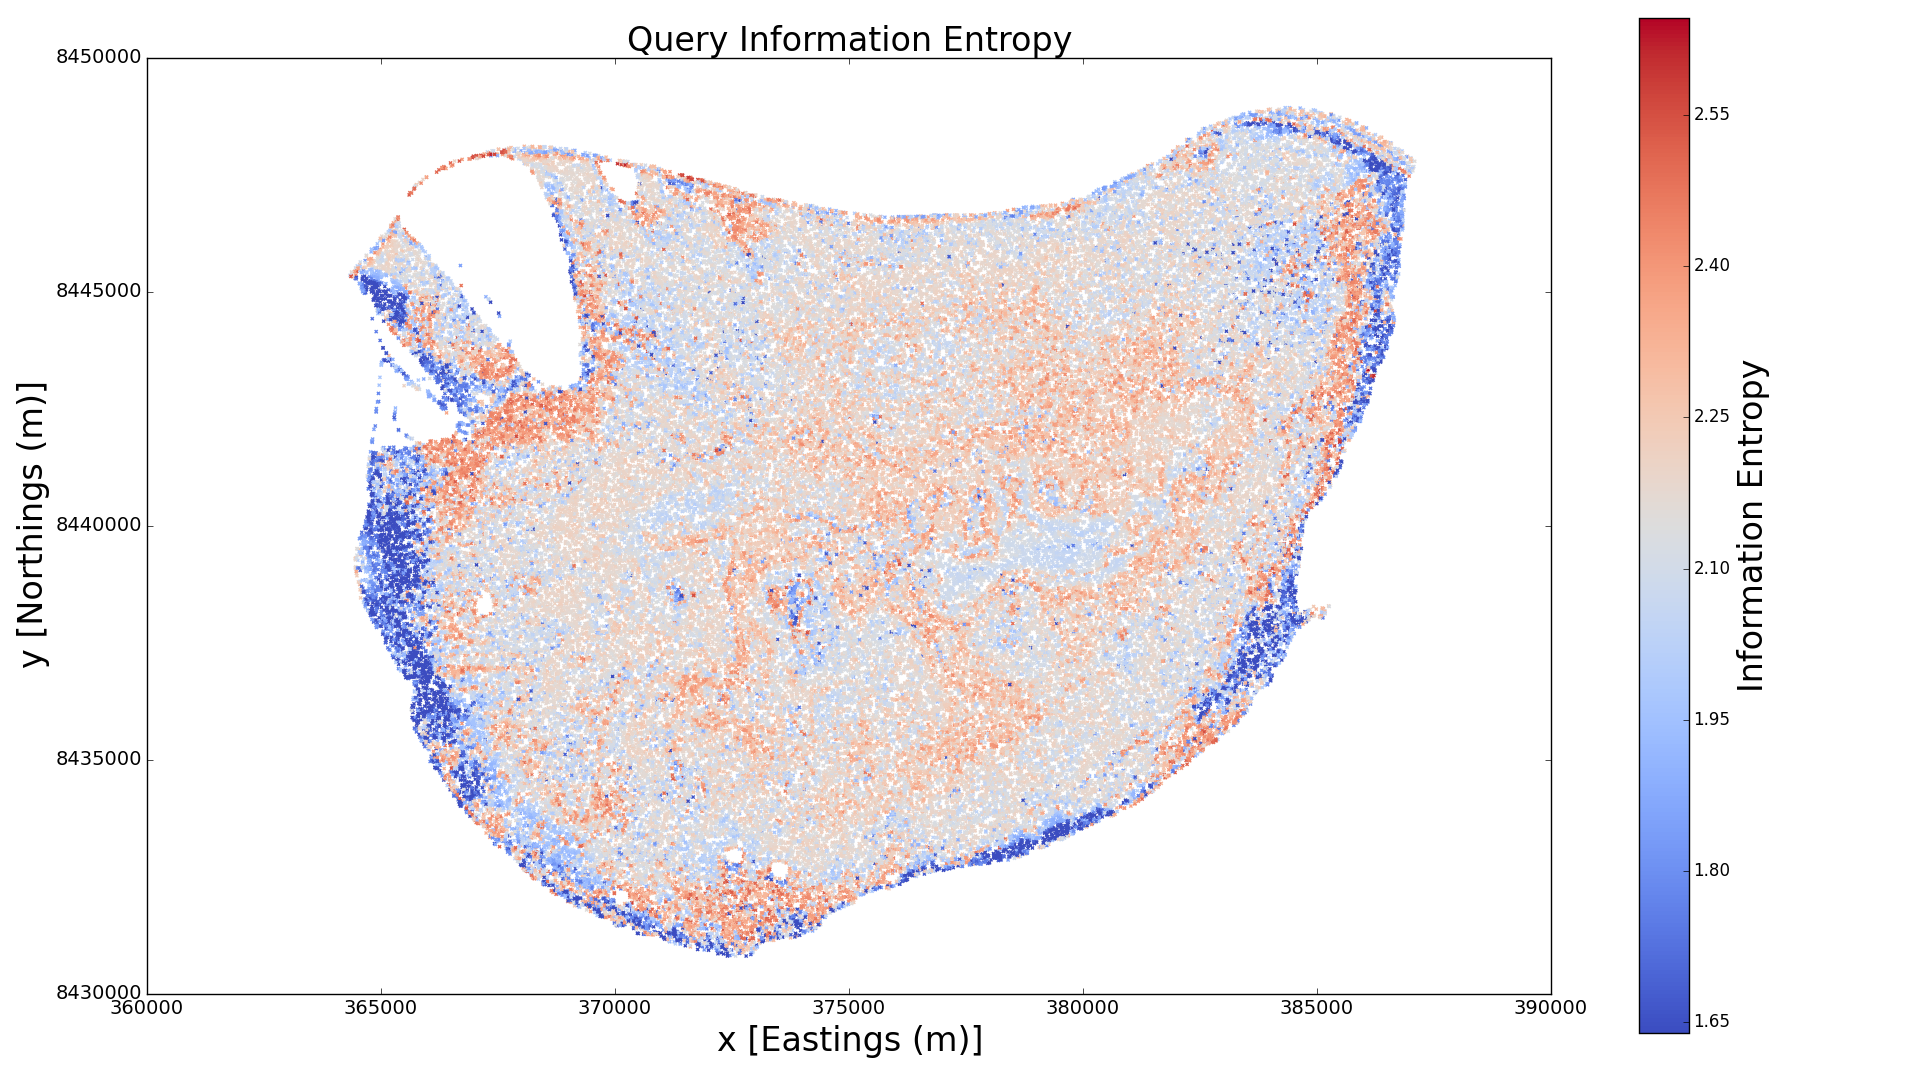
\includegraphics[width = 0.48\linewidth]{Figures/scott_reef_mapping/Figure9.eps}}
			  \subfigure[Linearised Model Differential Entropy]{\label{Figure:ScottReefLinearisedModelDifferentialEntropy}	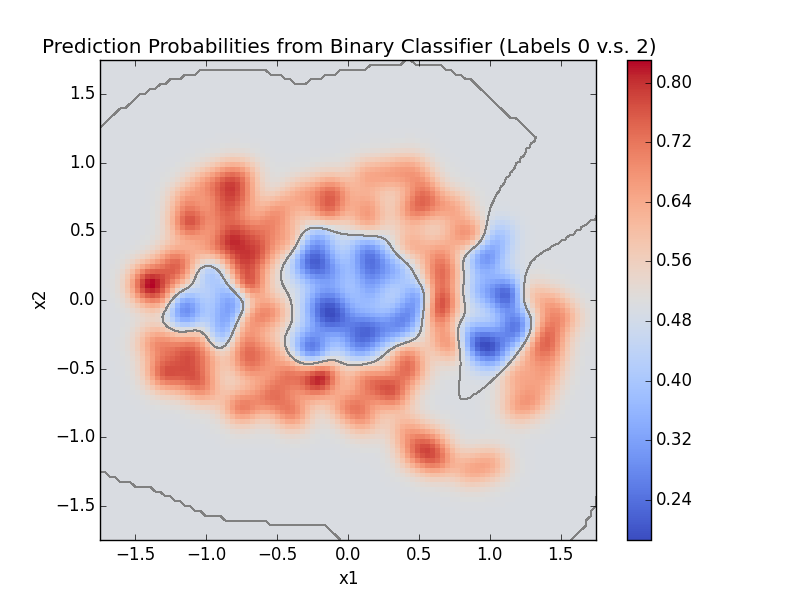
\includegraphics[width = 0.48\linewidth]{Figures//scott_reef_mapping/Figure11.eps}}
			\caption{Scott Reef: Initial Entropy Maps}
			\label{Figure:InitialEntropyMaps}
			\end{figure}
			
			LMDE acquisition, however, emphasizes on the places where the vehicle should first focus on (figure \ref{Figure:ScottReefLinearisedModelDifferentialEntropy}). Comparing Figure \ref{Figure:ScottReefLinearisedModelDifferentialEntropy} with the bathymetric features in Figure \ref{Figure:ScottReefBathymetricFeatures}, the marginalised LMDE is highest at places with the highest and lowest depths (figure \ref{Figure:ScottReefBathymetricFeatures:2}). While Figure \ref{Figure:ScottReefLinearisedModelDifferentialEntropy} only visualises the marginalised entropies, the fact that it is able to emphasize regions with marginalised entropies show that it is better equipped to also discern informative paths in the joint entropy case, leading to LMDE acquisition. Interestingly, the places with highest model variance matches the places with the lowest and highest depths, as it is on the edge of the feature space.
		
			The horizon structure selected for the Scott Reef scenario is 5 km in extent with 30 control points. Each control step is therefore $\frac{5 \mathrm{km}}{30}$ = 167 meters in length.  A comparison in performance over a distance of 33.3 km between several acquisition criterion is shown in Figure \ref{Figure:CompareMethods}. Each method is tested with a horizon length of 5 km starting at two distinct initial locations - (377.5, 8440.0) km and (380.0, 8440.0) km in Eastings-Northings frame. These locations will hereafter be referenced as ``location 1'' and ``location 2'' respectively. The acquisition criterion to be compared are linearised model differential entropy (LMDE), Monte Carlo prediction information entropy (MCPIE), one step ahead prediction information entropy (GREEDY-PIE), random walk (RANDOM), average of marginalised prediction information entropy (AMPIE), predetermined spiral path (SPIRAL), and predetermined line segmented paths (LINES). Of these, only LMDE and MCPIE acquisitions consider mutual information.
		
			\begin{table}[t]
				{\footnotesize
				\begin{center}
					\begin{tabular}{ l c c c c c c c }
					\hline
					Policy & LMDE & MCPIE & AMPIE & GREEDY-PIE & RANDOM & LINES & SPIRAL \\
					\hline
					Mutual & Yes & Yes & No & No & No & No & No \\
					Non-Myopic & Yes & Yes & Yes & No & No & Yes & Yes \\
					Informative & Yes & Yes & Yes & Yes & No & No & No \\
					\hline
					\end{tabular}
				\end{center}
				}
		  	\caption{Method Properties and Types}
		  	\label{Table:MethodProperties}			
		  	\end{table}	
		  	

		
%			\begin{figure}[!htbp]
%			\centering
%			  \subfigure[LMDE Acquisition]{\label{Figure:OptimalPathLMDE2} 
%			  	\includegraphics[width = 0.32\linewidth]{Figures/informative_seafloor_exploration/lmde/lde_propose1.eps}
%			  	\includegraphics[width = 0.32\linewidth]{Figures/informative_seafloor_exploration/lmde/lde_propose100.eps}
%			  	\includegraphics[width = 0.32\linewidth]{Figures/informative_seafloor_exploration/lmde/lde_propose200.eps}}
%			  \subfigure[MCPIE Acquisition]{\label{Figure:OptimalPathMCPIE2}	
%			  	\includegraphics[width = 0.32\linewidth]{Figures/informative_seafloor_exploration/mcpie/lde_propose1.eps}
%			  	\includegraphics[width = 0.32\linewidth]{Figures/informative_seafloor_exploration/mcpie/lde_propose100.eps}
%			  	\includegraphics[width = 0.32\linewidth]{Figures/informative_seafloor_exploration/mcpie/lde_propose200.eps}}
%			\caption{Scott Reef: Exploration paths}
%			\label{Figure:OptimalPaths2}
%			\end{figure}
%			
%			\begin{figure}[!htbp]
%			\centering
%			  \subfigure[LMDE Acquisition]{\label{Figure:OptimalPathLMDE3} 
%			  	\includegraphics[width = 0.32\linewidth]{Figures/informative_seafloor_exploration/lmde/pred_propose1.eps}
%			  	\includegraphics[width = 0.32\linewidth]{Figures/informative_seafloor_exploration/lmde/pred_propose100.eps}
%			  	\includegraphics[width = 0.32\linewidth]{Figures/informative_seafloor_exploration/lmde/pred_propose200.eps}}
%			  \subfigure[MCPIE Acquisition]{\label{Figure:OptimalPathMCPIE3}	
%			  	\includegraphics[width = 0.32\linewidth]{Figures/informative_seafloor_exploration/mcpie/pred_propose1.eps}
%			  	\includegraphics[width = 0.32\linewidth]{Figures/informative_seafloor_exploration/mcpie/pred_propose100.eps}
%			  	\includegraphics[width = 0.32\linewidth]{Figures/informative_seafloor_exploration/mcpie/pred_propose200.eps}}
%			\caption{Scott Reef: Exploration paths}
%			\label{Figure:OptimalPaths3}
%			\end{figure}
			
			There are several measures of performance criterion that can be used to measure performance. As the aim is to reduce misclassification rate, the percentage of misclassification across the map is compared between each method. It is important to understand that the misclassification rate is a rather harsh measure of the prediction performance, as any mismatch in prediction and ground truth is considered a misclassification. Unlike the regression case, there is no inherent measure of proximity in classification targets. For example, classifying \textit{Sand Biota 2} as \textit{Sand Biota 3} is penalised equally as classifying \textit{Sand Biota 2} as \textit{Dense Coral 1}, even though the first case is much more preferable. In this sense, the mapping accuracy is often in better in reality than the misclassification rate would suggest.
			
			Each method begins with the same scenario, for which the initial misclassification rate with 200 training points is 41.54\% (figure \ref{Figure:ScottReefInitialPredictions}). Table \ref{Table:CompareMethods} shows that, under this performance criterion, LMDE acquisition outperforms other exploration policies, with a final misclassification rate of 16.44\% and 20.38\% for location 1 and 2 respectively at the end of the journey. Methods LINES (20.40\% and 25.05\%) and MCPIE (22.29\% and 27.01\%) follow in performance. The predetermined line segmented paths (LINES) are chosen using after-the-fact knowledge through subjective judgement, and serve as an intuitive anchor for comparison. The MCPIE acquisition approach uses 1000 sample draws from the GP classifier to estimate the joint distribution for 30 control points, and experiences little improvement under misclassification criterion with more samples, as explained in Section \ref{InformativeSeafloorExploration:ComparisonMutualEntropyMeasures:EstimationAccuracy}. Notice that because LMDE acquisition prioritises on decision boundaries, it achieves a lower misclassification rate through appropriately reducing both bias and variance at decision boundaries.
			
			\begin{figure}[!htbp]
			\centering
			  \subfigure[LMDE Acquisition]{\label{Figure:FinalPredictionMapLMDE} \includegraphics[width = 0.48\linewidth]{Figures/informative_seafloor_exploration/lmde/pred200.eps}}
			  \subfigure[MCPIE Acquisition]{\label{Figure:FinalPredictionMapMCPIE}	\includegraphics[width = 0.48\linewidth]{Figures/informative_seafloor_exploration/mcpie/pred200.eps}}
			\caption{Scott Reef: Final Prediction Maps}
			\label{Figure:FinalPredictionMap}
			\end{figure}
		
			Figure \ref{Figure:FinalPredictionMap} shows the final predictions after 33.33 km under LMDE acquisition. The circle represents the horizon extent for which the vehicle considers in at each time step, with the vehicle at the center. The black path with small, coloured empty circles represent the path it has taken, and the path with filled hexagons extending from the current location represent the immediate proposed path from the receding horizon optimisation at that time.
					
			\begin{table}[t]
				{\footnotesize
				\begin{center}
					\begin{tabular}{ l c c c c c c c }
					\hline
					Policy & LMDE & MCPIE & AMPIE & GREEDY-PIE & RANDOM & LINES & SPIRAL \\
					\hline
					Location 1 & 16.44 & 22.99 & 32.11 & 43.86 & 34.87 & 20.40 & 33.74 \\
					Location 2 & 20.38 & 27.01 & 40.11 & 37.63 & 35.68 & 25.05 & 43.16 \\
					\hline
					\end{tabular}
				\end{center}
				}
		  	\caption{Final misclassification rate (\%)}
		  	\label{Table:CompareMethods}			
		  	\end{table}	
	  	
			As expected, the paths from the two methods are similar, with LMDE acquisition achieving a misclassification ratio of approximately 6.5\% less. Time lapse plots during the journey is shown in Appendix \ref{Appendix:SeafloorExplorationTimeLapse:Single}, where a more detailed analysis with respect to the prediction information entropy is provided.
			
			From the initial training set shown in Figure \ref{Figure:ScottReefBathymetricFeatures:1}, it is understood that observations are lacking around the edges of the reef. Moreover, Figures \ref{Figure:ScottReefBathymetricFeatures:2} to \ref{Figure:ScottReefBathymetricFeatures:6} reveals that the bathymetric signatures are quite different around the edges. For instance, the bathymetric depth is much lower, and the aspects are much higher. Therefore, it is expected that the AUV should focus on the edges of the reef. Note that from Figure \ref{Figure:ScottReefBathymetricFeatures:1} the shallowest regions of the region is still at least 23 meters in depth, which is still deep enough for exploration.
		
			\begin{figure}[!htbp]
			\centering
				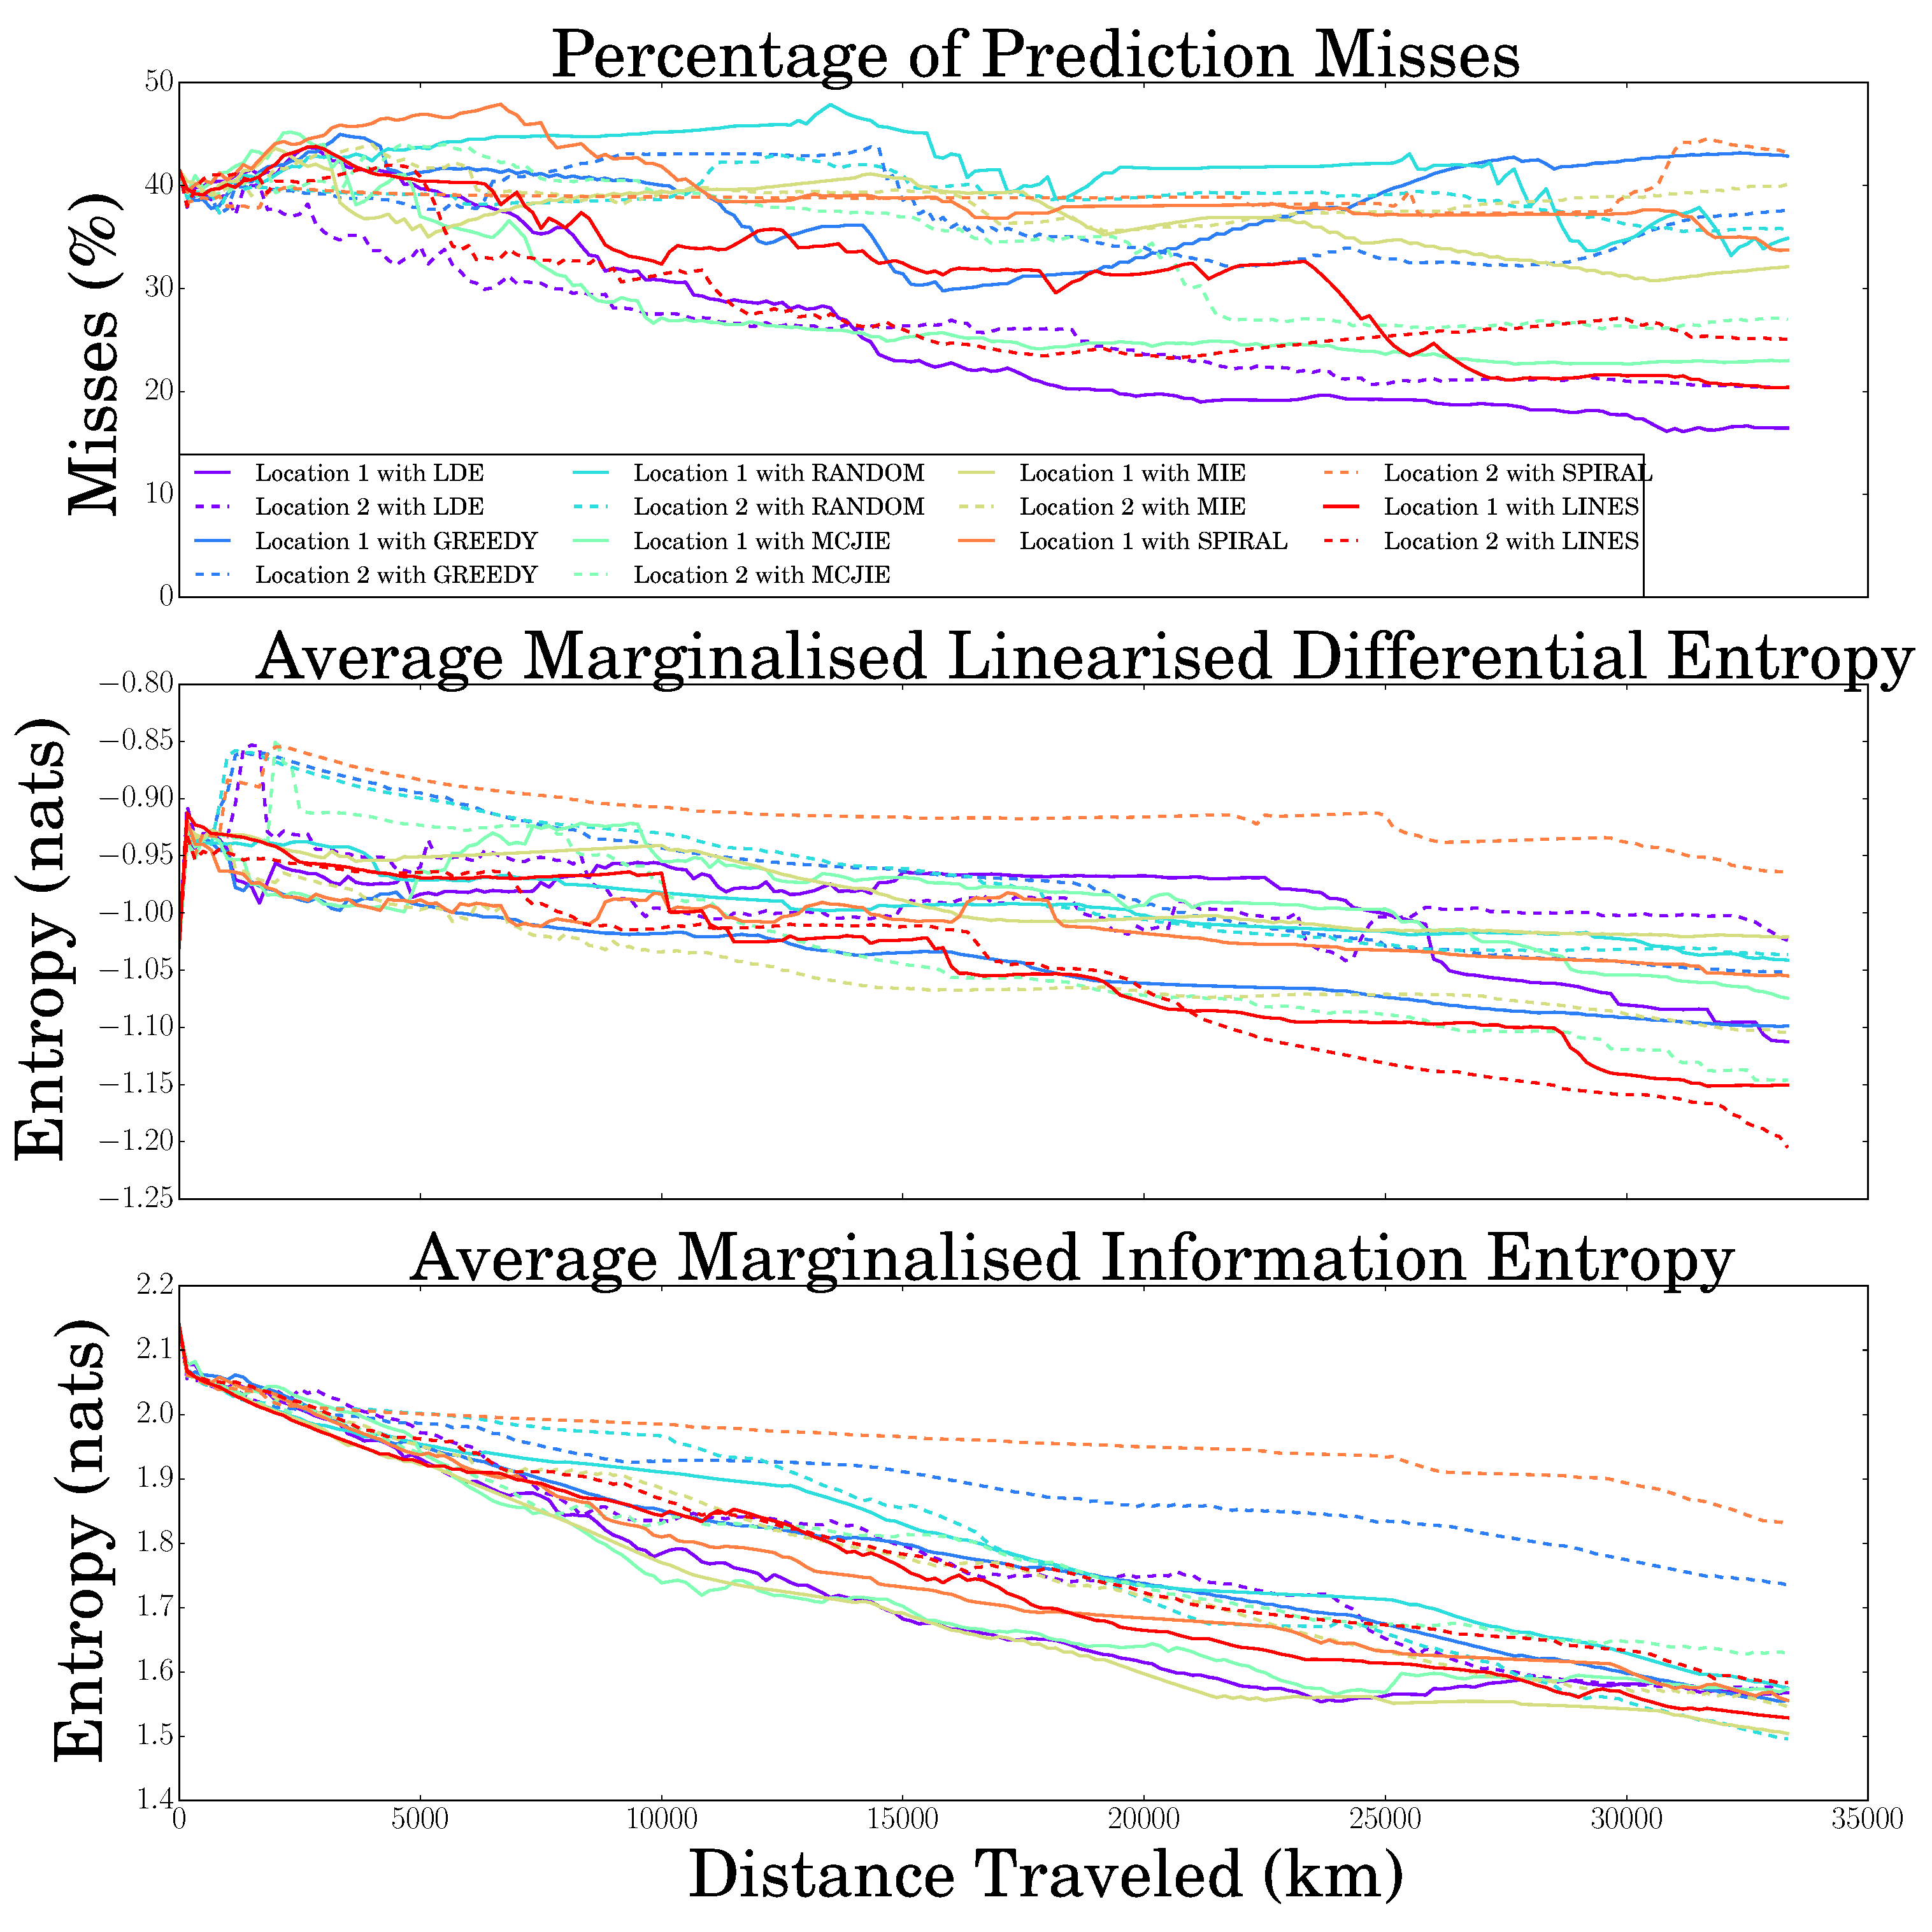
\includegraphics[width = 0.8\linewidth]{Figures/compare_methods.eps}
			\caption{Comparison of informative path planning policies}
			\label{Figure:CompareMethods}
			\end{figure}
				
			Unlike other methods, both the LMDE and MCPIE method take into consideration the mutual information of the proposed path, so that both methods outperform myopic or non-informative methods (figure \ref{Figure:CompareMethods} and table \ref{Table:MethodProperties}). This result demonstrates that under a receding horizon formulation, both LMDE and MCPIE acquisitions achieve lower misclassification rate on average than other exploration policies. Furthermore, a receding horizon method achieves lower misclassification rate than myopic approaches under the same acquisition function. Appendix \ref{Appendix:SeafloorExplorationTimeLapse:Single} also verifies the stability of LMDE acquisition through variance analysis.
				
		\subsection{Serial Mission Planning for Seafloor Exploration}
		\label{InformativeSeafloorExploration:ScottReef:SerialMission}
			
			Section \ref{InformativeSeafloorExploration:ScottReef:SingleMission} presented the case for a single mission that is 33.3 km in length. However, in practice the AUV would most likely run out of battery before such long length missions are completed. It is therefore more practical to deploy AUVs on multiple shorter missions, one after the another. Extra flexibility is introduced in this process where the next starting location can be chosen informatively from the observations collected thus far from the previous mission.
			
			As such, this section simulates a serial mission planning process for seafloor exploration, comparing the same set of exploration policies outlined previously. Figure \ref{Figure:ScottReefBathymetricFeatures:1} shows past mission tracks, which are usually more than 8 km in length. The following results assumes that the AUV is equipped with a conservative power supply that allows a mission length of 6.6 km. This distance is also chosen so that five such missions yield a total underwater distance covered of 33.3 km to allow qualitative comparisons against the single mission planning as shown previously. The AUV is to be picked up after each 6.6 km mission through a buoyant vehicle such as a boat, which can sail to the next starting location relatively quickly.
			
			Suppose the AUV is informatively exploring the seafloor using acquisition criterion $I$. After each 6.6 km mission, the AUV chooses the best location $\bvec{p}^{\star}$ to start from for the next mission through finding the region with the highest \textit{regional} acquisition value \eqref{Equation:SerialMissionOptimalLocation}. To allow for fair comparison of the regions, each region is composed of the same number of query points through a standard $k_{NN}$ algorithm.
			
			\begin{equation}
				\begin{aligned}
					\bvec{p}^{\star} &:= \argmax_{\bvec{p} \in \mathcal{P}} I[f_{k}(\bvec{p}) | X, \bvec{y}] \\
					f_{k}(\bvec{p}) &:= \{f_{e}(P) \quad | \quad P = k_{NN}(\bvec{p}, P_{r}, k) \}
				\end{aligned}
			\label{Equation:SerialMissionOptimalLocation}
			\end{equation}
			
			Here, $(X, \bvec{y})$ are the observations collected up to that mission. $k_{NN}(\bvec{p}, P_{r}, k)$ is the $k$-nearest-neighbour algorithm which finds the top $k$ points in $P_{r}$ that is closest to $\bvec{p}$ with respect to the standard Euclidean distance. Furthermore, instead of using the whole seafloor $P_{s}$, a finite subset $P_{r}$ of the $P_{s}$ is used to represent the seafloor to speed up computation. This means that only approximate optimal starting locations can be computed. In practical scenarios, however, this is sufficient.
			
			For the results below, $k = 10$ is chosen. $P_{r}$ is also sampled from $P_{s}$ such that for every point in $P_{r}$, there always exists another point in $P_{r}$ that is less than $100$ meters away. For methods non-informative methods, such as RANDOM, LINES, and SPIRAL, the starting points are then chosen randomly. 
			
			\begin{figure}[!htbp]
			\centering
			  \subfigure{\label{Figure:SerialMissionsSetup:Training}	\includegraphics[width=0.48\linewidth]{Figures/scott_reef_mapping_serial/figure1.eps}}
			  \subfigure{\label{Figure:SerialMissionsSetup:InitialMap}	\includegraphics[width=0.48\linewidth]{Figures/scott_reef_mapping_serial/figure8.eps}}
			  \subfigure{\label{Figure:SerialMissionsSetup:PIE-Map}	\includegraphics[width=0.48\linewidth]{Figures/scott_reef_mapping_serial/figure9.eps}}
			  \subfigure{\label{Figure:SerialMissionsSetup:LMDE-Map}	\includegraphics[width=0.48\linewidth]{Figures/scott_reef_mapping_serial/figure11.eps}}
			\caption{Serial Missions Setup}
			\label{Figure:SerialMissionsSetup}
			\end{figure}
			
			The added flexibility in serial mission scenario increases performance drastically. To make this more apparent, the initial starting scenario is composed of a minimal training dataset with 17 training points selected randomly from the dataset under the constraint that every training point has a different label (figure \ref{Figure:SerialMissionsSetup:Training}). While it is not necessary to start off with all the possible 17 labels, it enables efficient simulation as it allows corresponding caches to be easily allocated.
			
			The initial prediction map has poor accuracy, with 99.39\% classification miss ratio (figure \ref{Figure:SerialMissionsSetup:InitialMap}), as there are barely any observations to infer upon. Interestingly, the prediction uncertainty (figure \ref{Figure:SerialMissionsSetup:PIE-Map}) and model uncertainty (figure \ref{Figure:SerialMissionsSetup:LMDE-Map}) are almost opposite in trend. Specifically, the effect of bathymetric depth is again the most prominent through comparisons with Figure \ref{Figure:ScottReefBathymetricFeatures:2}. Note that the lowest and highest depths present in the initial training set are 31.69 m and 57.07 m, corresponding to labels \textit{Sand Biota 2} and \textit{Barron Sand 3}. As such, due to a squared exponential kernel, all the regions with depths lower than 31.69 m is predicted with \textit{Sand Biota 2} and all regions with depths higher than 57.07 m is predicted with \textit{Barron Sand 3}, as verified in Figure \ref{Figure:SerialMissionsSetup:InitialMap}. As such, the prediction uncertainty there is low, since there are no other observations to contradict this prediction (figure \ref{Figure:SerialMissionsSetup:PIE-Map}). However, because there is only one observation there, the model uncertainty is high at those points Figure \ref{Figure:SerialMissionsSetup:LMDE-Map}). This again shows that LMDE and PIE are complementary measures of entropy that measures different types of uncertainty.

			For comparison, all methods begin their mission at location 1. While LMDE and MCPIE acquisition produces two different resulting paths, the final prediction map achieved is very similar, with 18.30\% and 21.22\% misclassification ratio respectively (figures \ref{Figure:SerialFinalPredictionMapLMDE} and \ref{Figure:SerialFinalPredictionMapMCPIE}). Other informative exploration policies, AMPIE and GREEDY-PIE, also achieves reasonable mapping rate at 23.21\% and 37.54\% respectively after five 6.6 km missions (figures \ref{Figure:SerialFinalPredictionMapAMPIE} and \ref{Figure:SerialFinalPredictionMapGREEDY}). Compared to the initial scenario with 99.39\% misclassification rate, informative planning are able to achieve efficient mapping under five short missions.
			
			\begin{figure}[!htbp]
			\centering
			  \subfigure[LMDE Acquisition]{\label{Figure:SerialFinalPredictionMapLMDE} \includegraphics[width = 0.48\linewidth]{Figures/informative_seafloor_exploration/serial_lmde/pred199.eps}}
			  \subfigure[MCPIE Acquisition]{\label{Figure:SerialFinalPredictionMapMCPIE} \includegraphics[width = 0.48\linewidth]{Figures/informative_seafloor_exploration/serial_mcpie/pred199.eps}}
			  \subfigure[AMPIE Acquisition]{\label{Figure:SerialFinalPredictionMapAMPIE} \includegraphics[width = 0.48\linewidth]{Figures/informative_seafloor_exploration/serial_ampie/pred199.eps}}
			  \subfigure[GREEDY-PIE Acquisition]{\label{Figure:SerialFinalPredictionMapGREEDY} \includegraphics[width = 0.48\linewidth]{Figures/informative_seafloor_exploration/serial_greedy/pred199.eps}}
			\caption{Scott Reef: Final Prediction Maps}
			\label{Figure:SerialFinalPredictionMap}
			\end{figure}
			
			The same set of exploration policies are then compared in Figure \ref{Figure:SerialCompareMethods}, whose final misclassification rate is summarised in Table \ref{Table:SerialCompareMethods}. In this case, LMDE again outperforms other exploration policies, with MCPIE and AMPIE following closely. Note that this is a typical scenario and does not imply that LMDE acquisition always performs the best, but only most of the time. The performance is also highly dependent on the problem dataset, the ground truth, as well as the GP modelling choices itself. 

			\begin{table}[t]
				{\footnotesize
				\begin{center}
					\begin{tabular}{ l c c c c c c c }
					\hline
					Policy & LMDE & MCPIE & AMPIE & GREEDY-PIE & RANDOM & LINES & SPIRAL \\
					\hline
					Location 1 & 18.30 & 21.22 & 23.21 & 37.54 & 54.63 & 52.54 & 50.06 \\
					\hline
					\end{tabular}
				\end{center}
				}
		  	\caption{Final misclassification rate (\%)}
		  	\label{Table:SerialCompareMethods}
		  	\end{table}	
		  				
			\begin{figure}[!htbp]
			\centering
				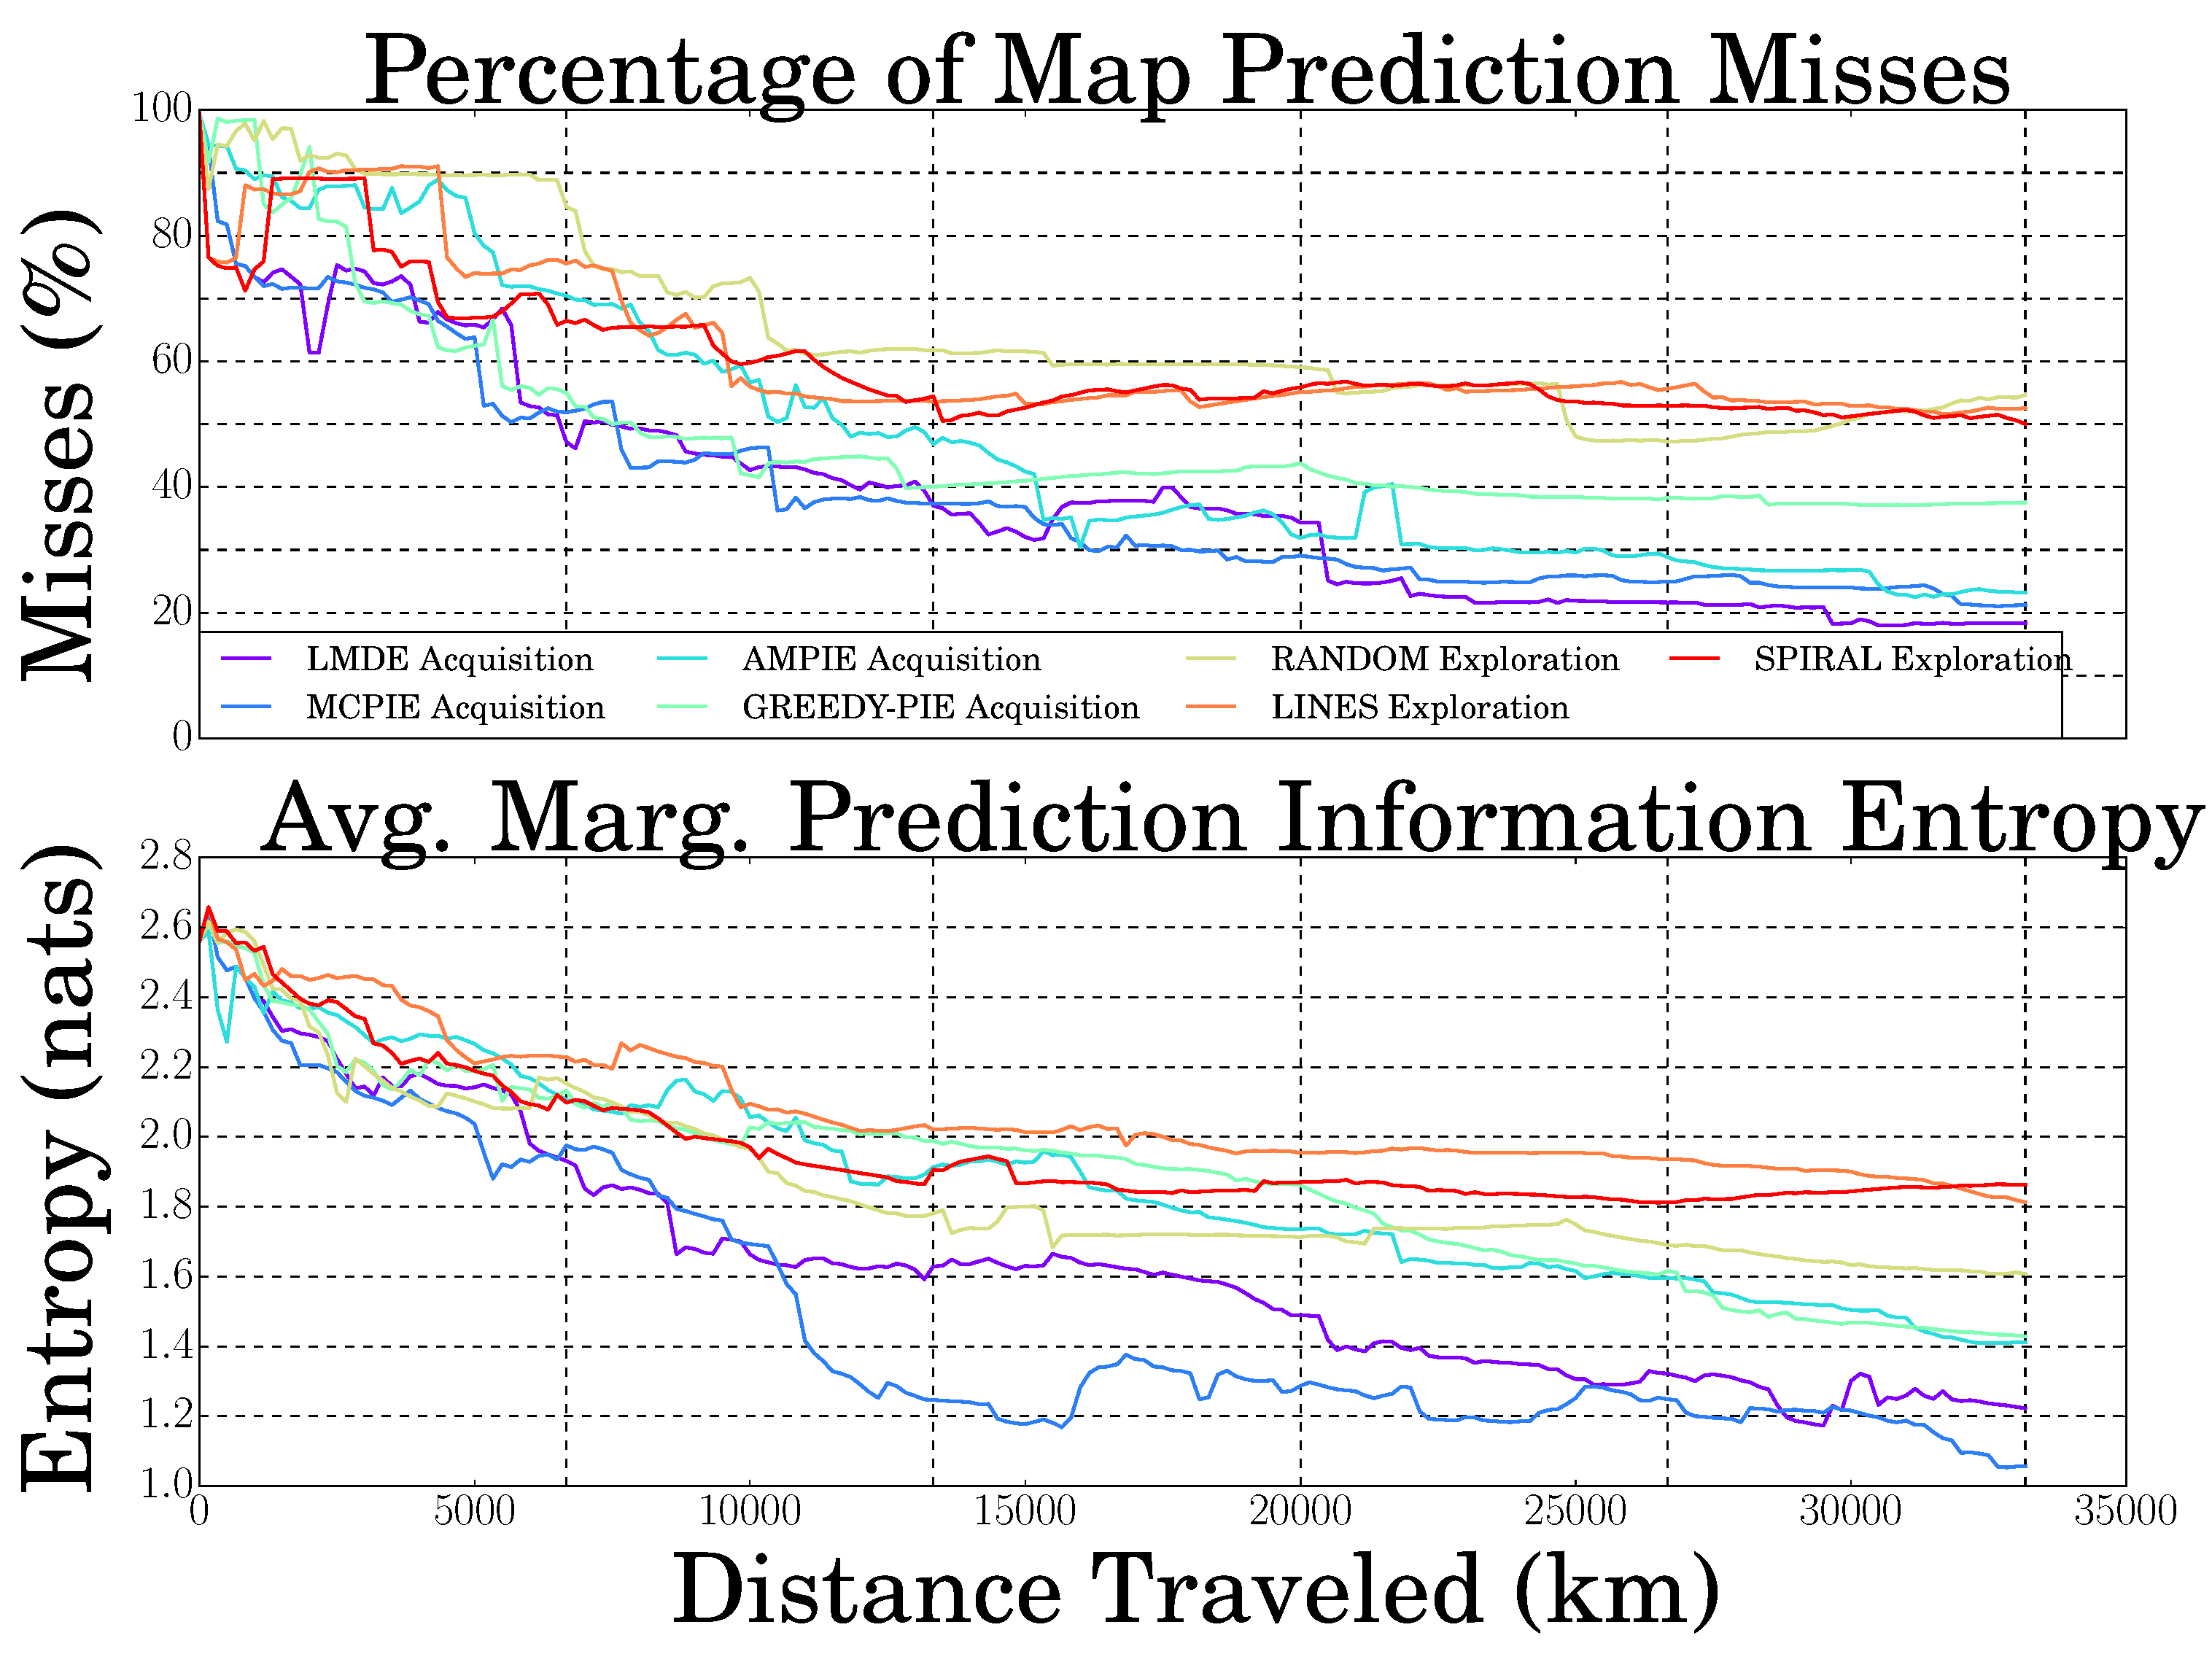
\includegraphics[width = 0.8\linewidth]{Figures/serial_compare_methods.eps}
			\caption{Comparison of informative path planning policies}
			\label{Figure:SerialCompareMethods}
			\end{figure}
						
			Nevertheless, Figure \ref{Figure:SerialCompareMethods} reveals that LMDE and MCPIE acquisitions under the receding horizon framework performs the best. Non-informative methods, however, is only able to achieve no more than 50\% mapping accuracy, with LMDE acquisition achieving more than 30\% mapping accuracy at the end of five missions. As such, simulations verifies the strength of non-myopic, informative path planing policies, and affirms the performance of mutual information measures, LMDE and MCPIE, as acquisition functions.
								
	\section{Summary}
	
		This chapter concludes the work in this thesis through verifying the performance of the two proposed acquisition criteria, LMDE acquisition and MCPIE acquisition. With a proposed receding horizon path planning scheme on the Scott Reef dataset, informative path planning with LMDE acquisition outperforms other methods under a mapping accuracy criteria.
		
		 
		
		
		

\chapter{Conclusion and Future Work}
\lhead{Conclusion and Future Work}
\label{Conclusion}

	This thesis investigates and develops informative seafloor exploration methods for benthic habitat mapping.
	
	After an introduction to the theory behind Bayesian modeling with Gaussian processes (Section \ref{Background:GaussianProcesses}), a review of current literature in informative path planning quickly reveals the need for a more computationally efficient approach that is non-myopic while capturing mutual information (Section \ref{Background:RelatedWork}).
	
	The outset of this thesis then begins by building upon the existing Gaussian process classification framework for benthic habitat mapping (Section \ref{BenthicHabitatMapping}). The benthic habitat mapping problem is first formulated as a supervised learning problem which requires the habitat labels to be modeled upon appropriate bathymetric features through classification. This requires an introduction to bathymetric features (Section \ref{BenthicHabitatMapping:BathymetricFeatures}). Through examining the usual binary classification framework, efficient and parallelisable multiclass classifiers are developed. The All versus All GP classifier is formulated in detail which parallels the way One versus All GP classifiers have been used in. Furthermore, on top of simple normalisation, two novel probability fusion methods, mode keeping and exclusion, are introduced which exhibit better inference properties with respect to computing the prediction information entropy (Section \ref{BenthicHabitatMapping:Classification}). The benthic habitats across the Scott Reef seafloor are then mapped with such classifiers which also provides the initial scenario for path planning to be used later on (Section \ref{BenthicHabitatMapping:ScottReef}).
	
	The work then moves on to investigate informative path planning methods that build upon such Gaussian process classifiers (Section \ref{InformativeSeafloorExploration}). Through motivating the need for a measure of mutual information, a direct approach with Monte Carlo estimation is formulated in order to compute the \textit{joint} prediction information entropy, hereby named Monte Carlo prediction information entropy (MCPIE) (Section \ref{InformativeSeafloorExploration:MCPIE}). Careful analysis of the predictive probabilities obtained under likelihood response transformations of the latent Gaussian process then inspires the concept of model differential entropy (MDE) of a Gaussian process classifier. Analytical tractability is then achieved through a linearisation technique for both the binary, multiclass OVA, and multiclass AVA scenario, thus producing the linearised model differential entropy (LMDE) mutual information measure (Section \ref{InformativeSeafloorExploration:LMDE}). The two measures are then compared in properties and performance, which reveals the complementary nature of the two mutual information measures that resembles the bias-variance trade-off that is ubiquitous in statistics and machine learning (Section \ref{InformativeSeafloorExploration:ComparisonMutualEntropyMeasures}).
	
	A stable and efficient path planning scheme is then developed under the receding horizon formulation (Section \ref{InformativeSeafloorExploration:RecedingHorizonFormulation}). While only optimal in finite horizon at each time instance, such an approach exhibits the following advantages compared to traditional informative path planning methods. Firstly, it avoids the need to compute acquisition criterion throughout the seafloor region, which is extremely costly in time for non-mutual information measures such as AMPIE, and furthurmore memory intensive for mutual information measures such as MCPIE and LMDE. As a result, this formulation make feasible the use of mutual information measures. Secondly, it allows a feedback structure to path planning and avoids executing outdated path plans. Thirdly, with an appropriate horizon structure, the method provides a balance between non-myopic planning and immediate feasibility.
	
	Finally, these acquisition criteria and informative path planning schemes are evaluated in performance with the Scott Reef dataset, which reveals the effectiveness of MCPIE and especially LMDE acquisition approaches over the AMPIE and GREEDY-PIE approaches, as well as non-informative methods (Section \ref{InformativeSeafloorExploration:ScottReef}).
	
	The work presented in this thesis calls for further work in improving and better evaluating the informative path planning methods proposed.
	
	One of the most important and intriguing is the relationship between prediction information entropy and model differential entropy. Semantic interpretations of their meanings have suggested that they are correspondingly similar to variance and bias, which are two sides of the ``coin'' of uncertainty. Further statistical analysis and investigation with probability theory could be interesting in revealing how these measures can be combined for a mutual information measure that allows the agent to intelligently discern uncertainty by variance and uncertainty by bias. With a hopeful outlook such a measure may be able to enable better acquisition properties for mapping problems that requires classification.
	
	On top of more investigations in the acquisition criteria, the path planning scheme itself can also be improved. The work of this thesis also follows the philosophy of transcribing a path planning problem in the continuous domain to the discrete domain. While this is a common approach, it is certainty superseded by techniques that allow planning directly in the original continuous domain, in order to avoid discretisation approximations and hence limitations. 
	
	Nevertheless, there are also immediate work that can be investigated which builds on the current discretised formulation. Firstly, the horizon length could be reduced as the agent reaches the end of each mission. As no missions will continue indefinitely, it may be beneficial to let the agent know that its mission will terminate shortly such that it will switch to a more greedy approach before its time is up. More important however are the choices of the mission length and stopping criteria. Currently, the missions lengths are chosen based on experiences with past missions and the power limitations of the AUV. Nevertheless, it can be interesting to investigate the case where the AUV itself decides when to stop a mission, surface to sea level, and have a ship deliver it to a new location where it finds the most informative. This is based on the fact that underwater velocities are much slower than surface velocities. Such a scheme would involve the AUV constantly evaluating its surroundings for potential information. With appropriately devised loss functions, the AUV would decide whether it has explored the current area enough such that it is time to move to a new area.
		
	The tractability and accuracy of the methods developed above can also be improved. In terms of tractability, one of the major limitations of this work is that the datasets are large in quantity. Much work has been done in the machine learning community for efficient approximations of Gaussian process inference, such as sparse Gaussian process approximations where weak kernel covariances are discarded to save both memory and computational time. In terms of accuracy, while Laplace approximation achieves good performance, there are other approximation techniques that produce even more accurate results, although unfortunately at the expense of higher time complexity. Examples of such approximation methods are Expectation Propagation and Variance Inference \cite{GaussianProcessForMachineLearning}.
	
	The work presented in this thesis is in fact not limited to the underwater domain. It can be used in any setting which requires building a map of discretely labeled objects. Typical examples are mapping the occupancy of an area, classifying between the objects such as cars and buildings, using an aerial monitoring system such as an unmanned aerial vehicle. Another application could be an autonomous ground vehicle building a map of the types of vegetation or environment distributed across an area. As such, the methods presented in this thesis could be tested on these scenarios to better evaluate performance, which can also serve to inspire ways of improvements as above.
	
	The above application domains also motivates the need for a spatial-temporal model. In the benthic habitat mapping scenario, it is assumed that the habitat map stay constant throughout the mapping procedure, so that observations made a long time ago are equally as valid as observations made recently. However, environmental monitoring problems such as simple occupancy mapping at a dynamic environment involve a dynamically changing ground truth. While spatial-temporal models based on Gaussian processes have been investigated before \cite{Roman:SequentialBayesianOptimisation}, these methods typically only address the mapping of continuous outputs which are regression type problems. Further work building upon the Gaussian process classification scheme developed is thus an interesting area to explore.
	
	

	

%% ----------------------------------------------------------------
% Now begin the Appendices, including them as separate files

\addtocontents{toc}{\vspace{2em}} % Add a gap in the Contents, for aesthetics

\appendix % Cue to tell LaTeX that the following 'chapters' are Appendices

\chapter{Computational Aspects of Gaussian Processes}
\lhead{Computational Aspects of Gaussian Processes}
\label{Appendix:ComputationalAspects}

	\section{Numerical Stability}
	\label{Appendix:ComputationalAspects:NumericalStability}
	
		\subsection{Cholesky Decomposition}
		\label{Appendix:ComputationalAspects:NumericalStability:Cholesky}

		\subsection{Cholesky Jittering}
		\label{Appendix:ComputationalAspects:NumericalStability:CholeskyJittering}
				
		\subsection{Solving Triangular Matrix Equations}
		\label{Appendix:ComputationalAspects:NumericalStability:SolvingTriangularMatrices}
		
		\subsection{Stable and Efficient Monte Carlo Sampling}
		\label{Appendix:ComputationalAspects:NumericalStability:MonteCarlo}
		
			Section \ref{InformativeSeafloorExploration:MCPIE} formulates the Monte Carlo prediction information entropy (MCPIE), which involves a Monte Carlo sampling stage for entropy estimation. In order to enhance the computational tractability of the approach, this thesis also investigates the practical implementation methods which would allow efficient computation for MCPIE.
			
			By definition of a GP, drawing from a GP at a \textit{finite} number of query points $X^{\star}$ is equivalent to drawing \textit{jointly} from a multivariate Gaussian distribution, as represented by \eqref{Equation:BinaryPredictiveGaussianDistribution} and \eqref{Equation:MulticlassPredictiveGaussianDistribution}. In general the sampling stage can be summarised by \eqref{Equation:GeneralMultivariateGaussianDistribution} for some mean vector $\vec{\upmu} \in \mathbb{R}^{n^{\star}}$ and covariance vector $\Sigma \in \mathbb{R}^{n^{\star} \times n^{\star}}$. 
			
			\begin{equation}
				{^{s}}\bvec{f}^{\star} \stackrel{\text{sample}}{\sim} \mathcal{N}(\vec{\upmu}^{\star}, \Sigma^{\star}) \qquad \forall s \in I_{n_{S}}
			\label{Equation:GeneralMultivariateGaussianDistribution}
			\end{equation}
			
			Note that $\stackrel{\text{sample}}{\sim}$ denotes that ${^{s}}\bvec{f}$ is not a random vector anymore but a specific vector after sampling. Instead of drawing jointly from the distribution \eqref{Equation:GeneralMultivariateGaussianDistribution} directly, a more advantageous approach involves first drawing \textit{iid} samples from the standard univariate normal distribution. That is, the samples are to be drawn independently.
			
			\begin{equation}
				\begin{aligned}
					z_{i, s} &\stackrel{\text{sample}}{\sim} \mathcal{N}(0, 1) \qquad \forall i \in I_{n^{\star}}, \forall s \in I_{n_{S}} \\
					\bvec{z}_{s} &:= \{z_{i, s}\}_{i \in I_{n^{\star}}} \in \mathbb{R}^{n^{\star}} \\
					Z &:= \{z_{i, s}\}_{i \in I_{n^{\star}}, \; s \in I_{n_{S}}} \equiv \begin{bmatrix} \bvec{z}_{1} & \bvec{z}_{2} & \dots & \bvec{z}_{n_{S}} \end{bmatrix} \in \mathbb{R}^{n^{\star} \times n_{S}}
				\end{aligned}
			\label{Equation:iidGaussianSampling}
			\end{equation}			
			
			Let $L^{\star}$ be the Cholesky Decomposition of $\Sigma^{\star}$, then $L^{\star} \bvec{z}_{s}$ incorporates the covariance structure \eqref{Equation:CovarianceInclusion}.
			
			\begin{equation}
				\begin{aligned}
					L^{\star} \bvec{z}_{s} \stackrel{\text{sample}}{\sim} \mathcal{N}(\bvec{0}, \Sigma^{\star}) \qquad \forall s \in I_{n_{S}}
				\end{aligned}
			\label{Equation:CovarianceInclusion}
			\end{equation}
			
			To incorporate the expectance $\vec{\upmu}^{\star}$, simple add it to the transformed samples \eqref{Equation:ExpectanceInclusion}.
			
			\begin{equation}
				\begin{aligned}
					\vec{\upmu}^{\star} + L^{\star} \bvec{z}_{s} \stackrel{\text{sample}}{\sim} \mathcal{N}(\vec{\upmu}^{\star}, \Sigma^{\star}) \qquad \forall s \in I_{n_{S}}
				\end{aligned}
			\label{Equation:ExpectanceInclusion}
			\end{equation}
			
			Therefore, to sample from any given multivariate Gaussian distribution $\mathcal{N}(\vec{\upmu}^{\star}, \Sigma^{\star})$, simply sample iid samples through \eqref{Equation:iidGaussianSampling} and transform the samples through \eqref{Equation:ExpectanceInclusion}, and set ${^{s}}\bvec{f}^{\star} := \vec{\upmu}^{\star} + L^{\star} \bvec{z}_{s} \quad \forall s \in I_{n_{S}}$. Generating iid samples from standard normal distributions is much faster, especially with sophisticated libraries which may have pseudo-random number generators specifically for values drawn from the standard normal distribution.
			
			Moreover, to vectorise the computation for further computational efficiency, multiple samples can be obtained at once through 
			
			\begin{equation}
				\begin{aligned}
					\begin{bmatrix} {^{1}}\bvec{f}^{\star} & {^{2}}\bvec{f}^{\star} & \dots & {^{n_{S}}}\bvec{f}^{\star} \end{bmatrix} &= \begin{bmatrix} \vec{\upmu}^{\star} + L^{\star} \bvec{z}_{1} & \vec{\upmu}^{\star} + L^{\star} \bvec{z}_{2} & \dots & \vec{\upmu}^{\star} + L^{\star} \bvec{z}_{n_{S}} \end{bmatrix} \\
					&= \mathcal{U} + L^{\star} Z \qquad \text{where} \qquad \mathcal{U} := \{\vec{\upmu}^{\star}\}^{T}_{s \in I_{n_{S}}}
				\end{aligned}
			\label{Equation:VectorisedSampling}
			\end{equation}			
			
	\section{Time Complexity}
	\label{Appendix:ComputationalAspects:TimeComplexity}
	
		Reducing computational time
		
%		\subsection{Numpy and Vectorisation}
		
		\subsection{Cholesky Update and Downdate}
		\label{Appendix:ComputationalAspects:TimeComplexity:CholeskyUpdateDowndate}
		
		\subsection{Caching learned GPs for fast prediction}
		
		\subsection{Parallelisation of GP learning and hyper-parameter batching}
		
		\subsection{Parallelisation of GP prediction and relevant subtleties}
		
%		\subsection{Fast vectorised GP drawing for regression and classification}
		
		
	\section{Time \& Spatial Complexity}
	\label{Appendix:ComputationalAspects:TimeSpaceComplexity}
	
		\subsection{Avoiding full covariance computations}
		\label{Appendix:ComputationalAspects:TimeSpaceComplexity:CovarianceAvoidance}
		
		\subsection{Taking advantage of diagonal log-likelihood Hessians}
		\label{Appendix:ComputationalAspects:TimeSpaceComplexity:DiagonalHessians}
		
		\subsection{Creating predictor objects to modularise prediction}
		
		 % Computational Aspects of Gaussian Processes
\chapter{Common Kernel Functions}
\lhead{Common Kernel Functions}
\label{Appendix:CommonKernelFunctions}

	While the squared exponential kernel suffices for most Gaussian process based inference, in general the choice of kernel covariance allows one to better adapt to the data at hand in order to achieve better predictive capabilities.
	
	This section extends the discussion in Section \ref{Background:GaussianProcesses:KernelFunctions} and covers the widely used \matern class kernels and the non-stationary Paciorek kernel. Again, the following discussion will only cover the minimal background for the structure and significance of kernel functions, as treatments of kernel functions can easily become very detailed and rigorous in topics such as differentiability effects or eigenfunction decomposition.
	
	\section{Other Stationary Kernels}
	\label{Appendix:CommonKernelFunctions:Stationary}
	
		Continuing with the formulation in Section \ref{Background:GaussianProcesses:KernelFunctions}, the \matern class of kernel functions are given by \eqref{Equation:MaternKernel}.
		
		\begin{equation}
			\left.
				\begin{aligned}
					k_{\mathrm{\maternmath}}(\bvec{x}, \bvec{x}') =& \; \sigma_{f}^{2} \frac{2^{1 - \nu}}{\Gamma(\nu)} \Big( \sqrt{2 \nu} a \Big)^{\nu} K_{\nu}\Big( \sqrt{2 \nu} a \Big) \\
					a^{2} :=& \; (\bvec{x} - \bvec{x}')^{T} \Sigma^{-1} (\bvec{x} - \bvec{x}')
				\end{aligned}
			\qquad \right.
		\label{Equation:MaternKernel}
		\end{equation}
					
		Here, $\Gamma$ and $K_{\nu}$ are the Gamma function and modified Bessel function respectively, while $\nu$ is a positive hyperparameter that determines the differentiability property of the \matern class kernel. The GP model with \matern class kernel is $d$-times mean square differentiable if and only if $\nu > d$ \citep{GaussianProcessForMachineLearning}. In the limit of $\nu \rightarrow \infty$ for infinite differentiability, the \matern kernel becomes the squared exponential kernel \eqref{Equation:SquaredExponentialKernel}. While the general \matern class kernel seem complicated due to the Gamma function and modified Bessel function, its form become simple for $\nu = p + \frac{1}{2}$ where $p$ is a non-negative integer. That is, \matern kernels with $\nu = \frac{1}{2}, \frac{3}{2}, \frac{5}{2}, \frac{7}{2}, \dots$ have simple analytic forms without reference to the modified Bessel function. In fact, for $\nu > \frac{5}{2}$, the degree for which the \matern kernel changes becomes quite unnoticeable for most practical purposes such that it may as well be replaced by the squared exponential kernel with $\nu \rightarrow \infty$. Similarly, while there is a more noticeable effect of changing $\nu$ within the range $\nu \in (0, \frac{5}{2})$, in practice is it is often not worth the expense of implementing the complicated form for an almost unnoticeable improvement in modeling accuracy. Hence, it is replaced with the \matern kernel with $\nu = \frac{1}{2}, \frac{3}{2}, \frac{5}{2}$, whichever is the closest. In this way, in practice only the \matern kernels with $\nu = \frac{1}{2}, \frac{3}{2}, \frac{5}{2}$ are employed, and they are respectively termed the \matern 1/2 kernel, \matern 3/2 kernel, and \matern 5/2 kernel - in the order of increasing differentiability. These kernels have the forms listed below \eqref{Equation:PracticalMaternKernels}.
		
		\begin{equation}
			\left.
				\begin{aligned}
					k_{\mathrm{\maternmath}, \; \nu = \frac{1}{2}}(\bvec{x}, \bvec{x}') =& \; \sigma_{f}^{2} \exp ( -a ) \\
					k_{\mathrm{\maternmath}, \; \nu = \frac{3}{2}}(\bvec{x}, \bvec{x}') =& \; \sigma_{f}^{2} (1 + \sqrt{3} a) \exp ( -\sqrt{3} a ) \\
					k_{\mathrm{\maternmath}, \; \nu = \frac{5}{2}}(\bvec{x}, \bvec{x}') =& \; \sigma_{f}^{2} \Big(1 + \sqrt{5} a + \frac{5}{3} a^{2}\Big) \exp ( -\sqrt{5} a )  \\
					a^{2} :=& \; (\bvec{x} - \bvec{x}')^{T} \Sigma^{-1} (\bvec{x} - \bvec{x}')
				\end{aligned}
			\qquad \right.
		\label{Equation:PracticalMaternKernels}
		\end{equation}			
		
		Together, the squared exponential kernel and the \matern class kernels provide a flexible set of kernel functions that can model a multitude of phenomena from various fields such as geology, ecology, finance, logistics, control theory, and machine learning.
		
	\section{Non-Stationary Kernels}
	\label{Appendix:CommonKernelFunctions:NonStationary}
	
		Non-stationary kernels introduce flexibility for modeling phenomenons where the inherent length scales varies across feature locations. The limitations with stationary kernels is that the GP will always learn length scales that are as small as it needs to be for modeling the fastest varying phenomenon in the model. While the marginal likelihood inherently balances modeling accuracy and overfitting, when it comes to the choice between modeling a peak in data variation with a risk of overfitting the rest of the data or ignoring that peak, the optimiser will always prefer the former as marginal likelihood gain from successful modeling is higher than loss from overfitting. Because learning stage is done through optimising the marginal likelihood (see Section \ref{Background:GaussianProcesses:Regression:HyperparameterLearning}), this forces the length scale to be smaller than it needs at slower varying places.

		Figure \ref{Figure:GaussianProcessLengthScale} illustrates the non-stationary Gaussian process for a terrain modeling application, where flat regions have high length scales (slow varying) while rough regions have low length scales (fast varying). Note that this does not imply that it is only relevant for GP regression problems - the latent functions used in GP classification is itself a GP regression problem for which length scale interpretation is almost identical to that shown in Figure \ref{Figure:GaussianProcessLengthScale}.
		
		\begin{figure}[!htbp]
			\centering
				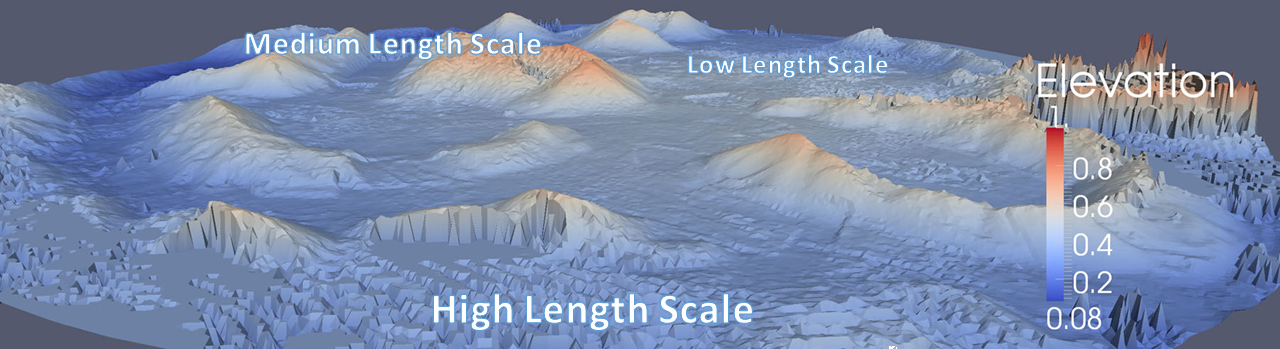
\includegraphics[width=\textwidth]{Figures/gaussianprocesslengthscale.png}
			\caption{Non-stationary Gaussian process for seafloor terrain modeling Adapted from \cite{ROB:ROB21403}}
			\label{Figure:GaussianProcessLengthScale}
		\end{figure}
		
		The non-stationary kernel function employed in this thesis is the Paciorek non-stationary covariance kernel function \eqref{Equation:NonStationaryKernel} \citep{AdaptiveNonStationaryKernel}.
		
		\begin{equation}
			k(\bvec{x}_{i}, \bvec{x}_{j}) = \sigma_{f}^{2} |\Sigma_{i}|^{\frac{1}{4}} |\Sigma_{j}|^{\frac{1}{4}} \Bigg|\frac{\Sigma_{i} + \Sigma_{j}}{2}\Bigg|^{-\frac{1}{2}} \exp\Bigg[ -\frac{1}{2} (\bvec{x}_{i} - \bvec{x}_{j}) \Bigg(\frac{\Sigma_{i} + \Sigma_{j}}{2}\Bigg)^{-1} (\bvec{x}_{i} - \bvec{x}_{j}) \Bigg]
		\label{Equation:NonStationaryKernel}
		\end{equation}			
		
		The matrices $\Sigma_{i}$ and $\Sigma_{j}$ are the local length scale matrices at $\bvec{x}_{i}$ and $\bvec{x}_{j}$ respectively, and are interpreted the same way as the stationary case. The only difference is that these length scale matrices only operate locally, and are functions of the input feature vector $\bvec{x}$. In each kernel location, two length scale matrices are queried. Hence, in a kernel matrix of size $n \times m$, maximally $n + m$ unique queries are made if no feature locations overlap.
		
		It is worthwhile to observe that the effective length scale matrix in the exponent is the average of the two length scale matrices, with its effect reduced with increasing distance between the two points of consideration as with all kernels.
		
		Note that the normalisation matrix determinants are chosen such that the kernel function is reduced into the squared exponential stationary kernel when $\Sigma_{i} = \Sigma_{j} = \Sigma$, as derived in \eqref{Equation:NonStationaryKernelToStationaryKernel}. 

		That is, the Paciorek non-stationary kernel reduces to the squared exponential kernel under the stationary limit. In this way, the Paciorek kernel generalises the squared exponential kernel.
				
		\begin{equation}
			\left.
				\begin{aligned}
					k(\bvec{x}_{i}, \bvec{x}_{j}) &= \sigma_{f}^{2} |\Sigma|^{\frac{1}{4}} |\Sigma|^{\frac{1}{4}} \Bigg|\frac{\Sigma + \Sigma}{2}\Bigg|^{-\frac{1}{2}} \exp\Bigg[ -\frac{1}{2} (\bvec{x}_{i} - \bvec{x}_{j}) \Bigg(\frac{\Sigma + \Sigma}{2}\Bigg)^{-1} (\bvec{x}_{i} - \bvec{x}_{j}) \Bigg] \\
					&= \sigma_{f}^{2} |\Sigma|^{\frac{1}{2}} |\Sigma|^{-\frac{1}{2}} \exp\Bigg[ -\frac{1}{2} (\bvec{x}_{i} - \bvec{x}_{j}) (\Sigma)^{-1} (\bvec{x}_{i} - \bvec{x}_{j}) \Bigg] \\
					&= \sigma_{f}^{2} \exp\Bigg[ -\frac{1}{2} (\bvec{x}_{i} - \bvec{x}_{j}) \Sigma^{-1} (\bvec{x}_{i} - \bvec{x}_{j}) \Bigg]
				\end{aligned}
			\qquad \right.
		\label{Equation:NonStationaryKernelToStationaryKernel}
		\end{equation}		
\chapter{Bathymetric Feature Extraction}
\lhead{Bathymetric Feature Extraction}
\label{Appendix:BathymetricFeatureExtraction}

	The following discussion details the ``Feature Extraction'' bubble in Figure \ref{Figure:InferenceFlow}. Given the bathymetric depth observations, the other bathymetric features, aspect and rugosity, can be computed in the short scale and long scale form in order to obtain a rich feature space for benthic habitat mapping.
	
	\section{Formulation}
	\label{Appendix:BathymetricFeatureExtraction:Formulation}
	
		With the basic structure of the benthic habitat mapping process in Section \ref{BenthicHabitatMapping:BathymetricFeatures}, the model spaces involved can be formulated as below.
		
		As established previously, the spatial space $\mathcal{P} \subseteq \mathbb{R}^{2}$ and feature space $\mathcal{X} \subseteq \mathbb{R}^{5}$ are compact subsets of $\mathbb{R}^{2}$ and $\mathbb{R}^{5}$ respectively. On the other hand, the habitat map space $\mathcal{Y} \subset \mathbb{N}$ is a strict finite subset of the the natural numbers, with each distinct integer representing a particular habitat type. Further, define $\mathscr{P} := \mathscr{P}(\mathcal{P})$, $\mathscr{X} := \mathscr{X}(\mathcal{X})$, and $\mathscr{Y} := \mathscr{Y}(\mathcal{Y})$ as the $\sigma$-algebras generated by $\mathcal{P} \subseteq \mathbb{R}^{2}$, $\mathcal{X} \subseteq \mathbb{R}^{5}$, and $\mathcal{Y} \subset \mathbb{N}$ respectively. Specifically, this means that $X \in \mathscr{X}$ implies $X \subseteq \mathcal{X}$, and similarly for $\mathscr{P}$ and $\mathscr{Y}$. Note that if $X := \{\bvec{x}_{i}\}_{i \in I_{n}} := \{\bvec{x}_{1}, \bvec{x}_{2}, \dots, \bvec{x}_{n}\} \in \mathscr{X}$ is a \textit{finite} collection of feature vectors $\bvec{x}_{i} \in \mathcal{X}$ for all $i \in I_{n}$, then $X$ is equivalent to the matrix $[\bvec{x}_{1}, \bvec{x}_{2}, \dots, \bvec{x}_{n}]^{T} \in \mathbb{R}^{n \times p}$. This notation is used consistently throughout, and a similar formulation applies to spatial coordinates $P \in \mathscr{P}$ and target labels $\bvec{y} := \{y_{i}\}_{i \in I_{n}} := \{y_{1}, y_{2}, \dots, y_{n}\} \in \mathscr{Y}$. Recall that for an arbitrary quantity $q_{i}$ indexed by $i \in I_{n}$, $\{q_{i}\}_{i \in I_{n}}$ is defined to be $\{q_{1}, q_{2}, \dots, q_{n}\}$ which is equivalent to a vector if $q_{i}$ is a scalar and a matrix if $q_{i}$ is a vector.
			
	\section{Data Matching on Real Datasets}
	\label{Appendix:BathymetricFeatureExtraction:DataMatching}
	
		A subtlety that arises from the above formulation is that during the training stage, the bathymetric data and the label data are not necessarily observed at the same places. Figure \ref{Figure:ScottReefBathymetricFeatures} illustrates the spatial distribution of the two datasets in a typical setting using the Scott Reef data set \citep{IMOS} as an example. Note that the colour scales have been shifted to emphasize the feature variations.
		
		Like the Scott Reef dataset, in most cases the bathymetric observations span the entire region of interest densely. However, while bathymetric data are usually collected rather uniformly and densely, the label data are collected from past AUV missions whose trajectory are continuous paths across a very limited region of the ocean floor \citep{Squidle}. As such, the label data are also spatially concentrated on the mission trajectory, while being almost non-existent elsewhere, making it a multi-modal distributed dataset. However, in order for the GP classifier to learn the relationship between the bathymetric features and habitat labels, the bathymetric and label data must have a one-to-one correspondence. That is, they must exist at the same locations. 
		
		Formally, let $P_{b}, P_{h} \in \mathscr{P}$ be the spatial positions at which bathymetric and label data have been observed. Let $X_{b} \in \mathscr{X}$ be the bathymetric features observed at $P_{b}$ and $\bvec{y}_{h} \in \mathscr{Y}$ be the habitat labels observed at $P_{h}$. The data matching problem is to obtain or infer $X_{h} \in \mathscr{X}$, the bathymetric features at locations $P_{h}$, from $X_{b}$. This is a standard supervised learning problem. Specifically, the aim is to learn an inference model $\zeta: P_{h} \mapsto X_{h}$ from the empirical relationship $P_{b} \mapsto X_{b}$.
		
		While it is possible to employ a separate GP regressor to perform the above inference, this adds unnecessary computational complexity. Since GPs are $O(n^{3})$ algorithms, using a layered GP approach where both stages of the benthic habitat mapping process employs GPs will increase the inference bottleneck. Instead, as there exists an abundance of bathymetric data, without much loss of accuracy it suffices to employ a nearest neighbour interpolation to obtain $X_{h}$. 
			
	\section{Aspect and Rugosity}
	\label{Appendix:BathymetricFeatureExtraction:DataMatching:AspectAndRugosity}
		
		The feature extraction process assumes that the bathymetric depth data is available in grid form. That is, one can represent the available depth data $Z = \{z_{k}\}_{k \in {1, 2, ..., N}}$ as $Z = \{z_{ij}\}_{i \in {1, 2, ..., n_{i}}, \;\; j \in {1, 2, ..., n_{j}}}$ where varying $i$ and $j$ corresponds to varying data points in axis 1 and 2 respectively. Axis 1 and 2 is required to form an orthonormal frame. While axis 1 and 2 is usually aligned with the eastings-northings frame, it is generally not required for the feature extraction process.
		
		Without loss of generality, let $x$ and $y$ denote quantities corresponding to the orthogonal axes. We have that at $(x_{i}, y_{j})$ $(i \in {1, 2, ..., n_{i}}, \;\; j \in {1, 2, ..., n_{j}})$ the depth is measured as $z_{ij}$. The partial derivatives of various degrees of accuracy and scale can then be estimated through central differencing. Table \ref{Table:AspectExtraction}  shows the case for extracting aspect in the $x$-direction. Correspondingly, replacing the operations from $i$ to $j$ the aspect in the $y$-direction can also be similarly extracted.
		
		\bgroup
		\def\arraystretch{2}%  1 is the default, change whatever you need
		\begin{table}[t]
			\begin{center}
				\begin{tabular}{ c c }
					\hline
					\hline
					N & Aspect (Slope) Extraction [$x$-direction]\\
					\hline
					\hline
					3 & $^{3}_{x}a_{i, j} := \frac{- z_{i - 1, j} + z_{i + 1, j}}{2h}$ \\
					5 & $^{5}_{x}a_{i, j} := \frac{z_{i - 2, j} - 8 z_{i - 1, j} + 8 z_{i + 1, j} - z_{i + 2, j}}{12h}$ \\
					7 & $^{7}_{x}a_{i, j} := \frac{-z_{i - 3, j} + 9 z_{i - 2, j} - 45 z_{i - 1, j} + 45 z_{i + 1, j} - 9 z_{i + 2, j} + z_{i + 3, j}}{60h}$ \\
					9 & $^{9}_{x}a_{i, j} := \frac{3 z_{i - 4 j} - 32 z_{i - 3, j} + 168 z_{i - 2, j} - 672 z_{i - 1, j} + 672 z_{i + 1, j} - 168 z_{i + 2, j} + 32 z_{i + 3, j} - 3 z_{i + 4, j}}{840h}$ \\
					\hline
					\hline
				\end{tabular}
			\end{center}
	  	\caption{Aspect feature extraction using finite (central) difference approximations}
	  	\label{Table:AspectExtraction}			
	  	\end{table}	
	 		\egroup
	 		
	 		The chosen spacing employed in this thesis are $N = 3$ neighbors for short scale aspect and $N = 9$ neighbors for large scale aspect. That is, \begin{align*} \numberthis \label{Equation:AspectExtraction}
	 				{_{x}\{a_{s}\}_{i, j}} &:= {^{3}_{x}a_{i, j}} \quad && {_{y}\{a_{s}\}_{i, j}} := {^{3}_{y}a_{i, j}} \quad && {\{a_{s}\}_{i, j}} := \sqrt{{_{x}\{a_{s}\}^{2}_{i, j}} + {_{y}\{a_{s}\}^{2}_{i, j}}} \\
	 				{_{x}\{a_{l}\}_{i, j}} &:= {^{9}_{x}a_{i, j}} \quad && {_{y}\{a_{l}\}_{i, j}} := {^{9}_{y}a_{i, j}} \quad && {\{a_{l}\}_{i, j}} := \sqrt{{_{x}\{a_{l}\}^{2}_{i, j}} + {_{y}\{a_{l}\}^{2}_{i, j}}}
	 		\end{align*}
	 						  					
		Central differencing is chosen as it is more numerically accurate. The disadvantages of instability and slightly higher time complexity from dynamic cases are not present in the static feature extraction process. Nevertheless, forward differencing is to be used at the boundaries of the dataset where neighboring data is missing on one side.
					
		With two axis, the result is a 2 element gradient vector. It is possible to treat the 2 elements as separate features. However, this would make the modeling problem frame dependent which would unnecessarily complicate the modeling process. Therefore, the magnitude of this gradient is taken as the aspect feature \eqref{Equation:AspectExtraction}. 
		
		Rugosity is a measure of local height variations in the terrain. By definition, it is computed with $r = A_{r}/A_{g}$, the real surface area divided by the geometric surface area. Under bathymetry measurements that are geo-referenced through stereo imagery, rugosity can be calculated through a Delaunay triangulated surface mesh and projecting areas onto the plane of best fit using Principal Component Analysis (PCA) \citep{Friedman:Rugosity}.
		
		In the case that the bathymetric data is sufficiently sparse or is not distributed uniformly for grid based methods, then the above feature extraction process becomes inaccurate or even infeasible so that feature extraction itself becomes a prediction problem. When this happens, a Gaussian process regression model is proposed for predicting the features at a given spatial location. While this is much more computationally expensive than performing feature extraction, it is also quite rare that this is necessary under abundant bathymetric data. In most cases, it suffices to simply take the nearest neighbouring feature.
		
		In the benthic habitat mapping scenario, however, part of the reason that bathymetric features are used in the beginning is that bathymetric data is abundant and relatively densely observed. Therefore, it is rare to find a case where the above feature extraction does not apply.
		
		After each feature is extracted, each feature can then be whitened, or standardised, in order to allow better numerical properties for the classifier to model the benthic habitats upon the bathymetric features. While this is not necessarily, it ensures that each feature are roughly in the same numerical range so that no particular feature would dominate the model simply due to differences in the orders of magnitude. To standardise, each training feature set is subtracted by its mean and divided by its standard deviation, which are referred to as the \textit{whiten parameters}. The query feature set then undergoes the same transformation using the whiten parameters from the training set to allow uniform transformations.
		
		
		
%\chapter{Approximation Performance of Gaussian Process Classifiers}
\lhead{Approximation Performance of Gaussian Process Classifiers}
\label{Appendix:ApproximationPerformance}


\chapter{Mutual Entropy Measures}
\lhead{Mutual Entropy Measures}
\label{Appendix:MutualEntropyMeasures}

	This section supports the analysis in Section \ref{InformativeSeafloorExploration:ComparisonMutualEntropyMeasures} by providing the corresponding results for the multiclass case.
	
	The tests cases are setup in the same way as the binary classification scenario in Section \ref{InformativeSeafloorExploration:ComparisonMutualEntropyMeasures:EstimationAccuracy}. An OVA multiclass classifier is used (section \ref{BenthicHabitatMapping:Classification:MulticlassClassification:OVA}), and the probabilities are fused using the \textit{exclusion} method (section  \ref{BenthicHabitatMapping:Classification:Multiclass:ProbabilityFusion}).

	\begin{figure}[!htbp]
		\centering
			\includegraphics[width = \linewidth]{Figures/mcpie_lmde_comparison_multiclass/mcpie_lmde_comparison.eps}
		\caption{GP multiclass classifier example}
		\label{Figure:mcpie_lmde_comparison_multiclass}
	\end{figure}
		
	In summary, the results are consistent with the observations with the binary case, in that linearised model differential entropy better captures the decision boundaries and places without observations more distinctly than the usual prediction information entropy (figure \ref{Figure:mcpie_lmde_comparison_multiclass}). Furthermore, it also takes around more than 1000 samples for the Monte Carlo prediction information entropy to converge to the true prediction information entropy (figure \ref{Figure:mcpie_accuracy_multiclass}).
	
	\begin{figure}[!htbp]
		\centering
			\includegraphics[width = \linewidth]{Figures/mcpie_lmde_comparison_multiclass/mcpie_accuracy.eps}
		\caption{Accuracy improvement of MCPIE for a multiclass case}
		\label{Figure:mcpie_accuracy_multiclass}
	\end{figure}
\chapter{Problems and Solutions to Big Data}
\lhead{Problems and Solutions to Big Data}
\label{Appendix:BigData}

		\section{Benthic Habitat Mapping}
		\label{Appendix:BigData:BenthicHabitatMapping}
		
			One of the problems of performing inference on big datasets is that it has high memory and time complexity requirements. In the current Scott Reef example, there are a total of $n = 34890$ training points and $n^{\star} = 17675180$ query points, even after removing all invalid entries. With regards to the training stage, since Gaussian processes are $O(n^{3})$ algorithms, the high number of training points will cause learning bottlenecks in the process.
			
			More importantly, however, is the memory requirements involved in the inference stage. As explained in sections \ref{Background:GaussianProcesses:Regression} and \ref{BenthicHabitatMapping:Classification}, the inference stage requires the computation of a data kernel $K \in \mathbb{R}^{n \times n}$, an inference kernel $K^{\star} \in \mathbb{R}^{n \times n^{\star}}$, and a query kernel $K^{\star \star} \in \mathbb{R}^{n^{\star} \times n^{\star}}$. Since $n^{\star}$ is orders of magnitude greater than $n$, the memory requirements are dominated by $K^{\star \star}$. Fortunately, in the mapping scenario, it is not necessary to know the covariances between all the query points. Merely the variances at each query point needs to be known such that only the diagonal elements of $K^{\star \star}$ is required, which is $n^{\star}$ in length. The details of this computational shortcut is detailed in appendix \ref{Appendix:ComputationalAspects:TimeSpaceComplexity:CovarianceAvoidance}. However, the full inference kernel $K^{\star}$ is required in order to relate the training points to the query points, without which no inference can be performed. The inference kernel has $n \times n^{\star} = 616687030200 \approx 6 \times 10^{11}$ elements. Even if 32 bit floats instead of 64 bit floats are used, each element takes 32 bits = 4 bytes of memory, such that the total memory requirement for the inference kernel using the entire dataset would be $616687030200 \times 4$ bytes $\approx 2297$ GB \textit{for each binary classifier}. With an OVA classifier for 17 labels, this means more than 39 TB of storage is needed, which is infeasible to store on a standard computer of 4 to 16 GB RAM.
			
			As such, it is imperative to perform analysis with a sample of the dataset. As this section also serves to demonstrate the situation before a path planning mission is initiated, small numbers of training points will be chosen to reflect the high uncertainty in the resulting map due to a lack of data. In the following sections, $n = 200$ training points and $n^{\star} = 100000$ query points are randomly selected from the dataset for map inference, which forms the effective training data $(P, X, \bvec{y})$ and query data $(P^{\star}, X^{\star})$.
			
		\section{Informative Seafloor Exploration}
		\label{Appendix:BigData:InformativeSeafloorExploration}
		
			Similar to the problems faced in benthic habitat mapping as discussed in Section \ref{BenthicHabitatMapping:ScottReef:BigData}, big data also poses significant problems for informative path planning.
			
			As many of the acquisition functions discussed in Section \ref{Background:RelatedWork:AcquisitionFunctions} is based on the average marginalised prediction information entropy (AMPIE) \eqref{Equation:AMPIE}, which does not consider mutual information, the entropy computation can be improved in temporal and spatial complexity through only computing the latent GP variance $\{\mathbb{V}[f^{\star}_{i}]\}_{i \in I_{n^{\star}}}$ shown in Figure \ref{Figure:InferenceFlow} (see appendix \ref{Appendix:ComputationalAspects:TimeSpaceComplexity:CovarianceAvoidance}). As such, acquisition criterions such as \eqref{Equation:AsherBenderAcquisitionCriterion} and \eqref{Equation:KrauseAcquisitionCriterion} are able to consider the non-mutual entropy of the entire region of interest $X_{s}$. The memory requirement in this case is dominated by the inference kernel $K^{\star}$ as only the diagonal elements of the query matrix $K^{\star \star}$ are required. 
			
			However, if mutual information is required, then the entire latent covariance matrix $\mathbb{V}[\bvec{f}^{\star}]$ is required. The memory requirement is then dominated by the full query kernel $K^{\star \star}$ on top of the inference kernel $K^{\star}$. It would then be impractical to compute those covariance matrices for the entire region of interest $X_{s}$. That is, it would be impractical to compute the differential acquisition \eqref{Equation:DifferentialAcquisition} for either $H = H_{\mathrm{MCPIE}}$ or $H = H_{\mathrm{LMDE}}$.
			
			\begin{equation}
				I[X_{p} | X, \bvec{y}, X_{s}] = H[X_{s} | X, \bvec{y}] - H[X_{s} | X \cup X_{p}, \bvec{y} \cup \mathbb{E}[\bvec{y}_{p}]]
			\label{Equation:DifferentialAcquisition}
			\end{equation}
			
			Instead, the advantage of LMDE acquisition is that the acquisition criterion can be in the form of \eqref{Equation:PathAcquisition}. In other words, this searches for the path with maximal entropy. In the following section, this acquisition criterion form will be used for LMDE, MCPIE, and AMPIE acquisition, where the entropy measure $H$ is replaced by $H_{\mathrm{LMDE}}$, $H_{\mathrm{MCPIE}}$, and $H_{\mathrm{AMPIE}}$ respectively. That is, the acquisition criterion is to maximise the chosen entropy measure of the candidate path.

			\begin{equation}
				I[X_{p} | X, \bvec{y}, X_{s}] = H[X_{p} | X, \bvec{y}]
			\label{Equation:PathAcquisition}
			\end{equation}
			
\chapter{Seafloor Exploration Time Lapse}
\lhead{Seafloor Exploration Time Lapse}
\label{Appendix:SeafloorExplorationTimeLapse}

	\section{Single Mission Planning for Seafloor Exploration}
	\label{Appendix:SeafloorExplorationTimeLapse:Single}
	
			\begin{figure}[!htbp]
			\centering
			  \subfigure[LMDE Acquisition]{\label{Figure:OptimalPaths:LMDE} 
			  	\includegraphics[width = 0.32\linewidth]{Figures/informative_seafloor_exploration/lmde/mie_propose1.eps}
			  	\includegraphics[width = 0.32\linewidth]{Figures/informative_seafloor_exploration/lmde/mie_propose100.eps}
			  	\includegraphics[width = 0.32\linewidth]{Figures/informative_seafloor_exploration/lmde/mie_propose200.eps}}
			  \subfigure[MCPIE Acquisition]{\label{Figure:OptimalPaths:MCPIE}	
			  	\includegraphics[width = 0.32\linewidth]{Figures/informative_seafloor_exploration/mcpie/mie_propose1.eps}
			  	\includegraphics[width = 0.32\linewidth]{Figures/informative_seafloor_exploration/mcpie/mie_propose100.eps}
			  	\includegraphics[width = 0.32\linewidth]{Figures/informative_seafloor_exploration/mcpie/mie_propose200.eps}}
			\caption{Scott Reef: Exploration paths}
			\label{Figure:OptimalPaths}
			\end{figure}
			
			Figures \ref{Figure:OptimalPaths} show snapshots of the resulting path under LMDE and MCPIE acquisition respectively. Since in the end it is the prediction accuracy, instead of the model accuracy, that determines mapping and classification accuracy, the paths are layered onto the prediction information entropy (PIE) map for this visualisation. The snapshots are taken at 0.17 km (1\%), 16.67 km (50\%), and 33.33 km (100\%) into the journey.

			Under LMDE acquisition, as seen in Figure \ref{Figure:OptimalPaths:LMDE}, the AUV starts from the reef center, travels to the reef edge, returns from the reef edge to observe another inner region, and finally continues to map the reef edge. On the other hand, in Figure \ref{Figure:OptimalPaths:MCPIE}, the AUV simply travels to the reef edge and continues to observe the edges under MCPIE acquisition. As such, both methods focuses on the edges of the reef. However, LMDE acquisition did not neglect other regions while focusing on the reef edge, as it understands that too many observations at similar bathymetric signatures will introduce bias in the model.
			
			This difference is visible through the lower amount of prediction information entropy around the inner regions of the reef under LMDE acquisition compared to MCPIE acquisition, demonstrating better prediction accuracy. Interestingly, although MCPIE acquisition is the joint form of prediction information entropy, it is LMDE acquisition that achieves lower overall prediction information entropy. As discussed in Section \ref{InformativeSeafloorExploration:ComparisonMutualEntropyMeasures:EstimationAccuracy}, while MCPIE acquisition focuses on prediction variance, LMDE acquisition focuses on model variance which translate to both prediction variance and bias. Hence, in general, LMDE acquisition achieves better performance in the long run.

			\begin{figure}[!htbp]
			\centering
			  \subfigure[Initial Starting Positions]{\label{Figure:CompareLocations}	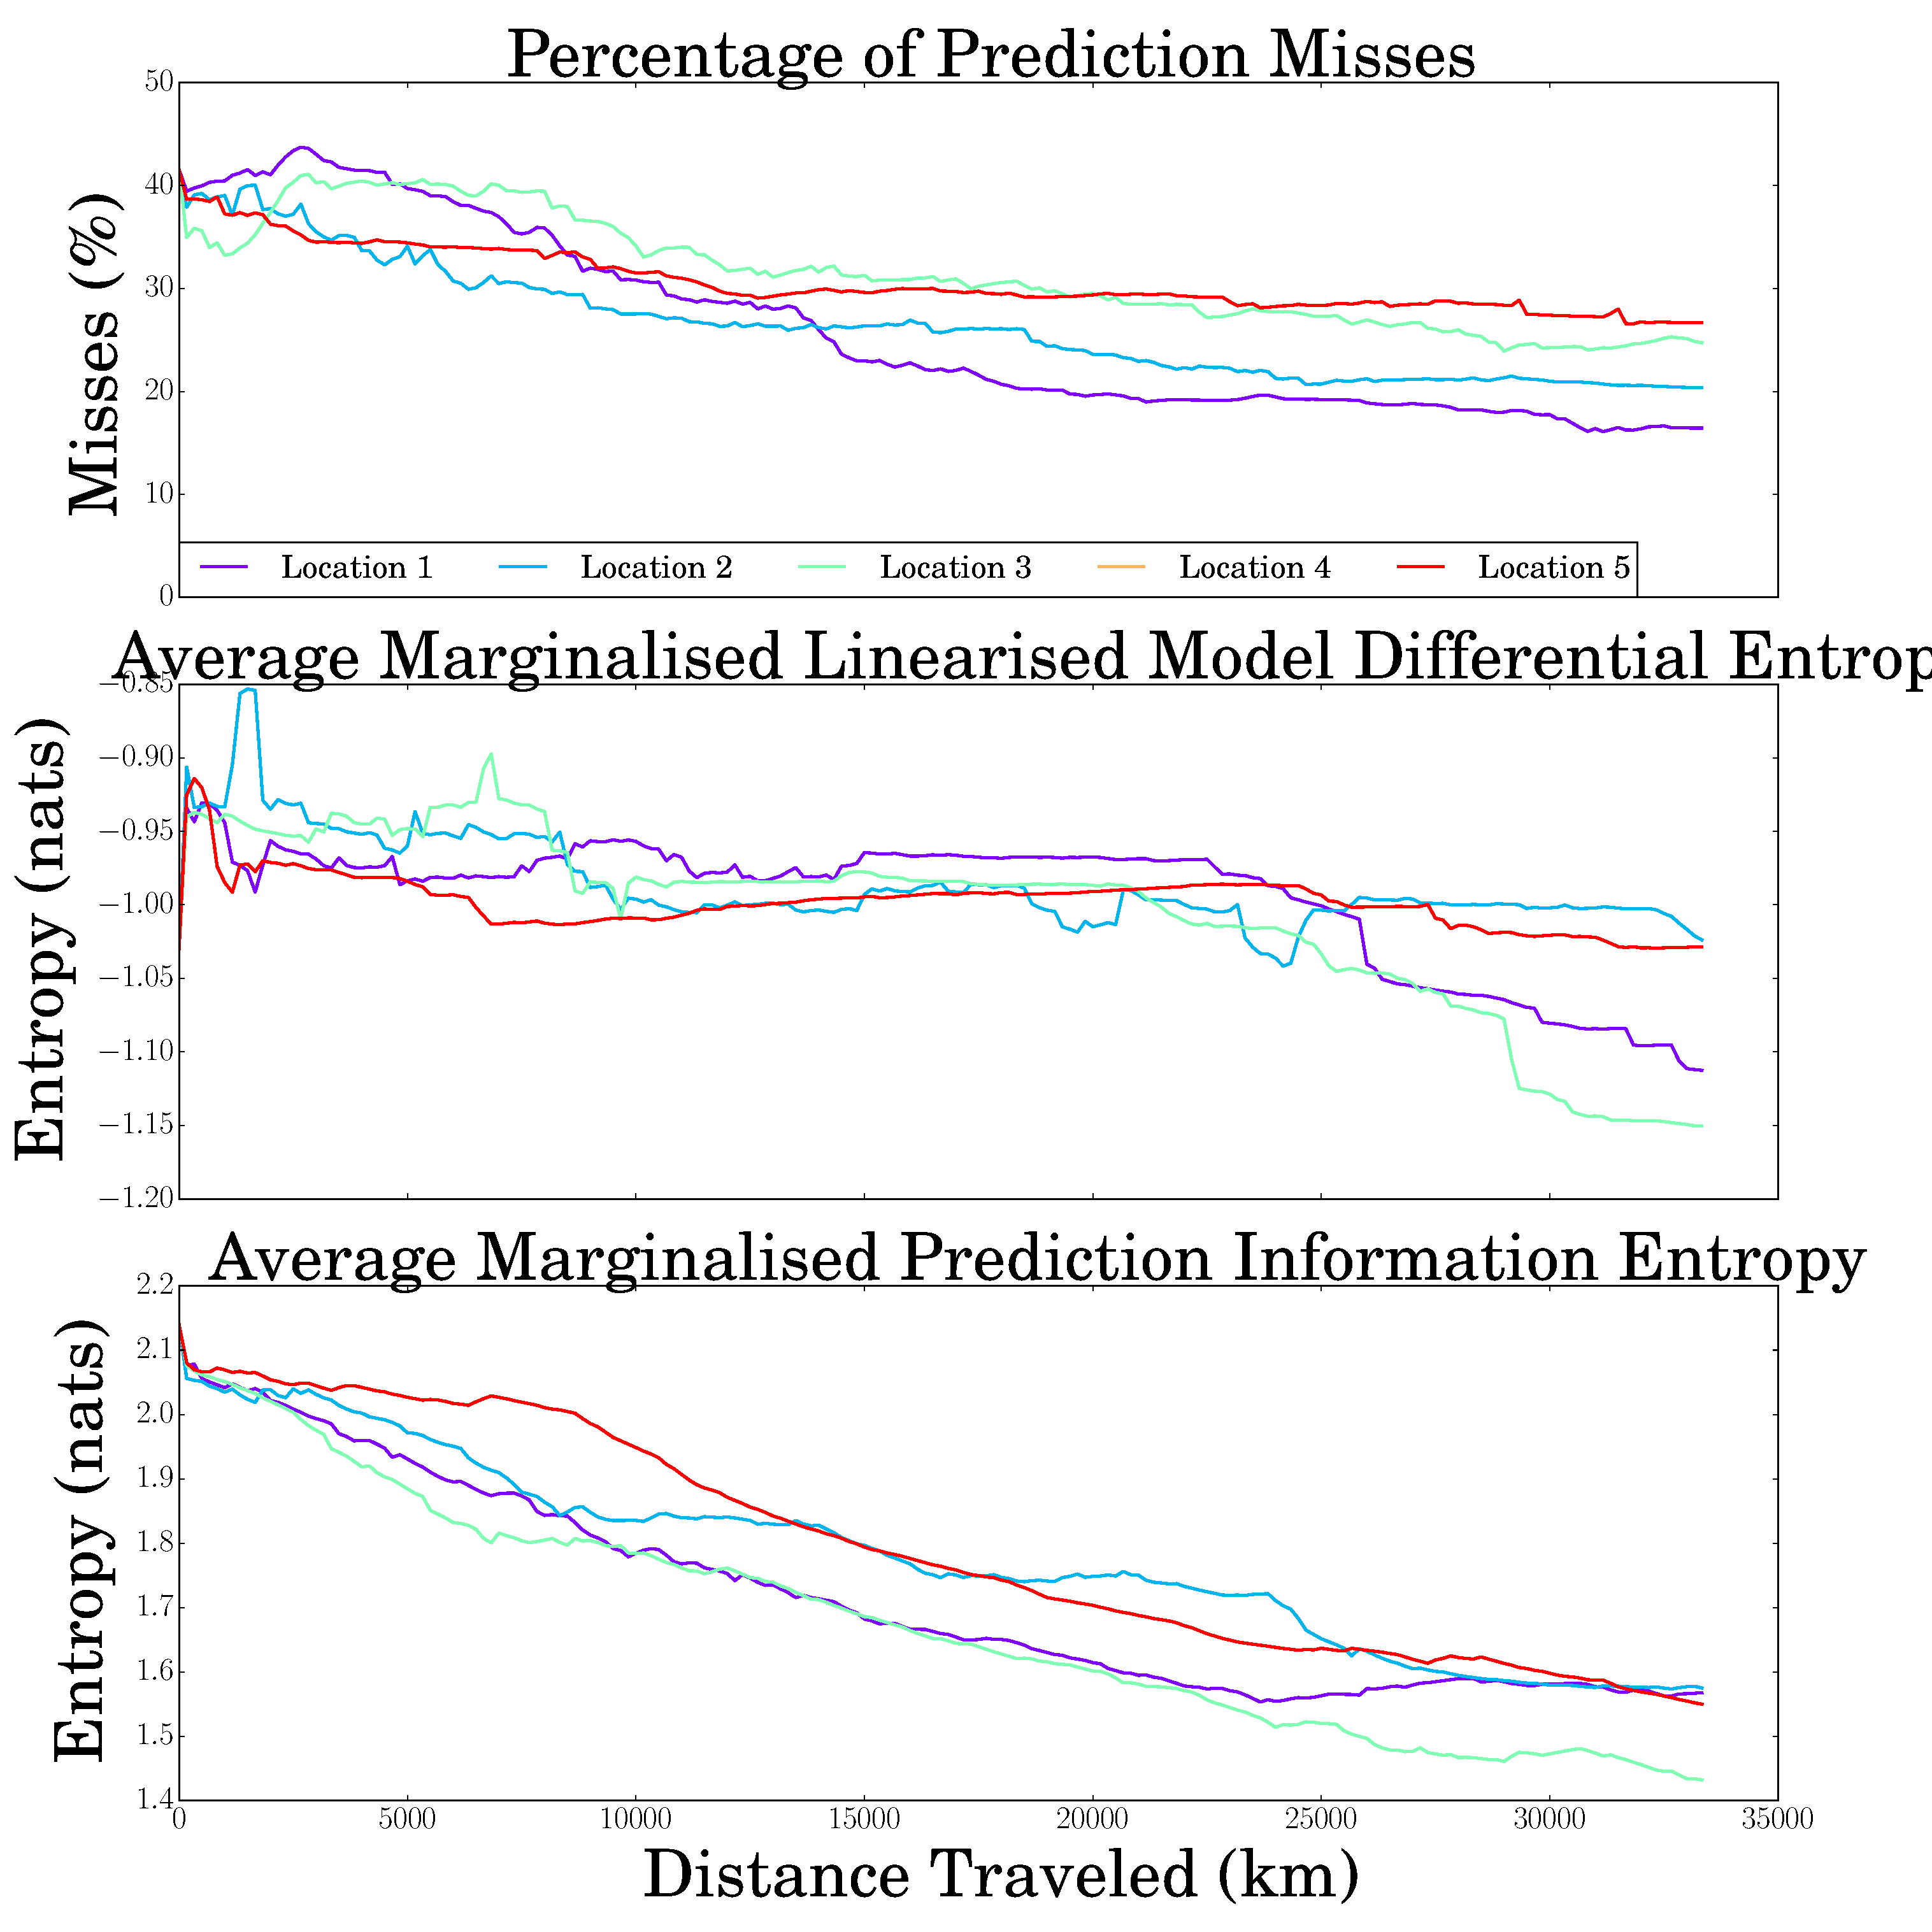
\includegraphics[width=0.48\linewidth]{Figures/compare_locations.eps}}
			  \subfigure[Receding Horizon Lengths]{\label{Figure:CompareHorizons}	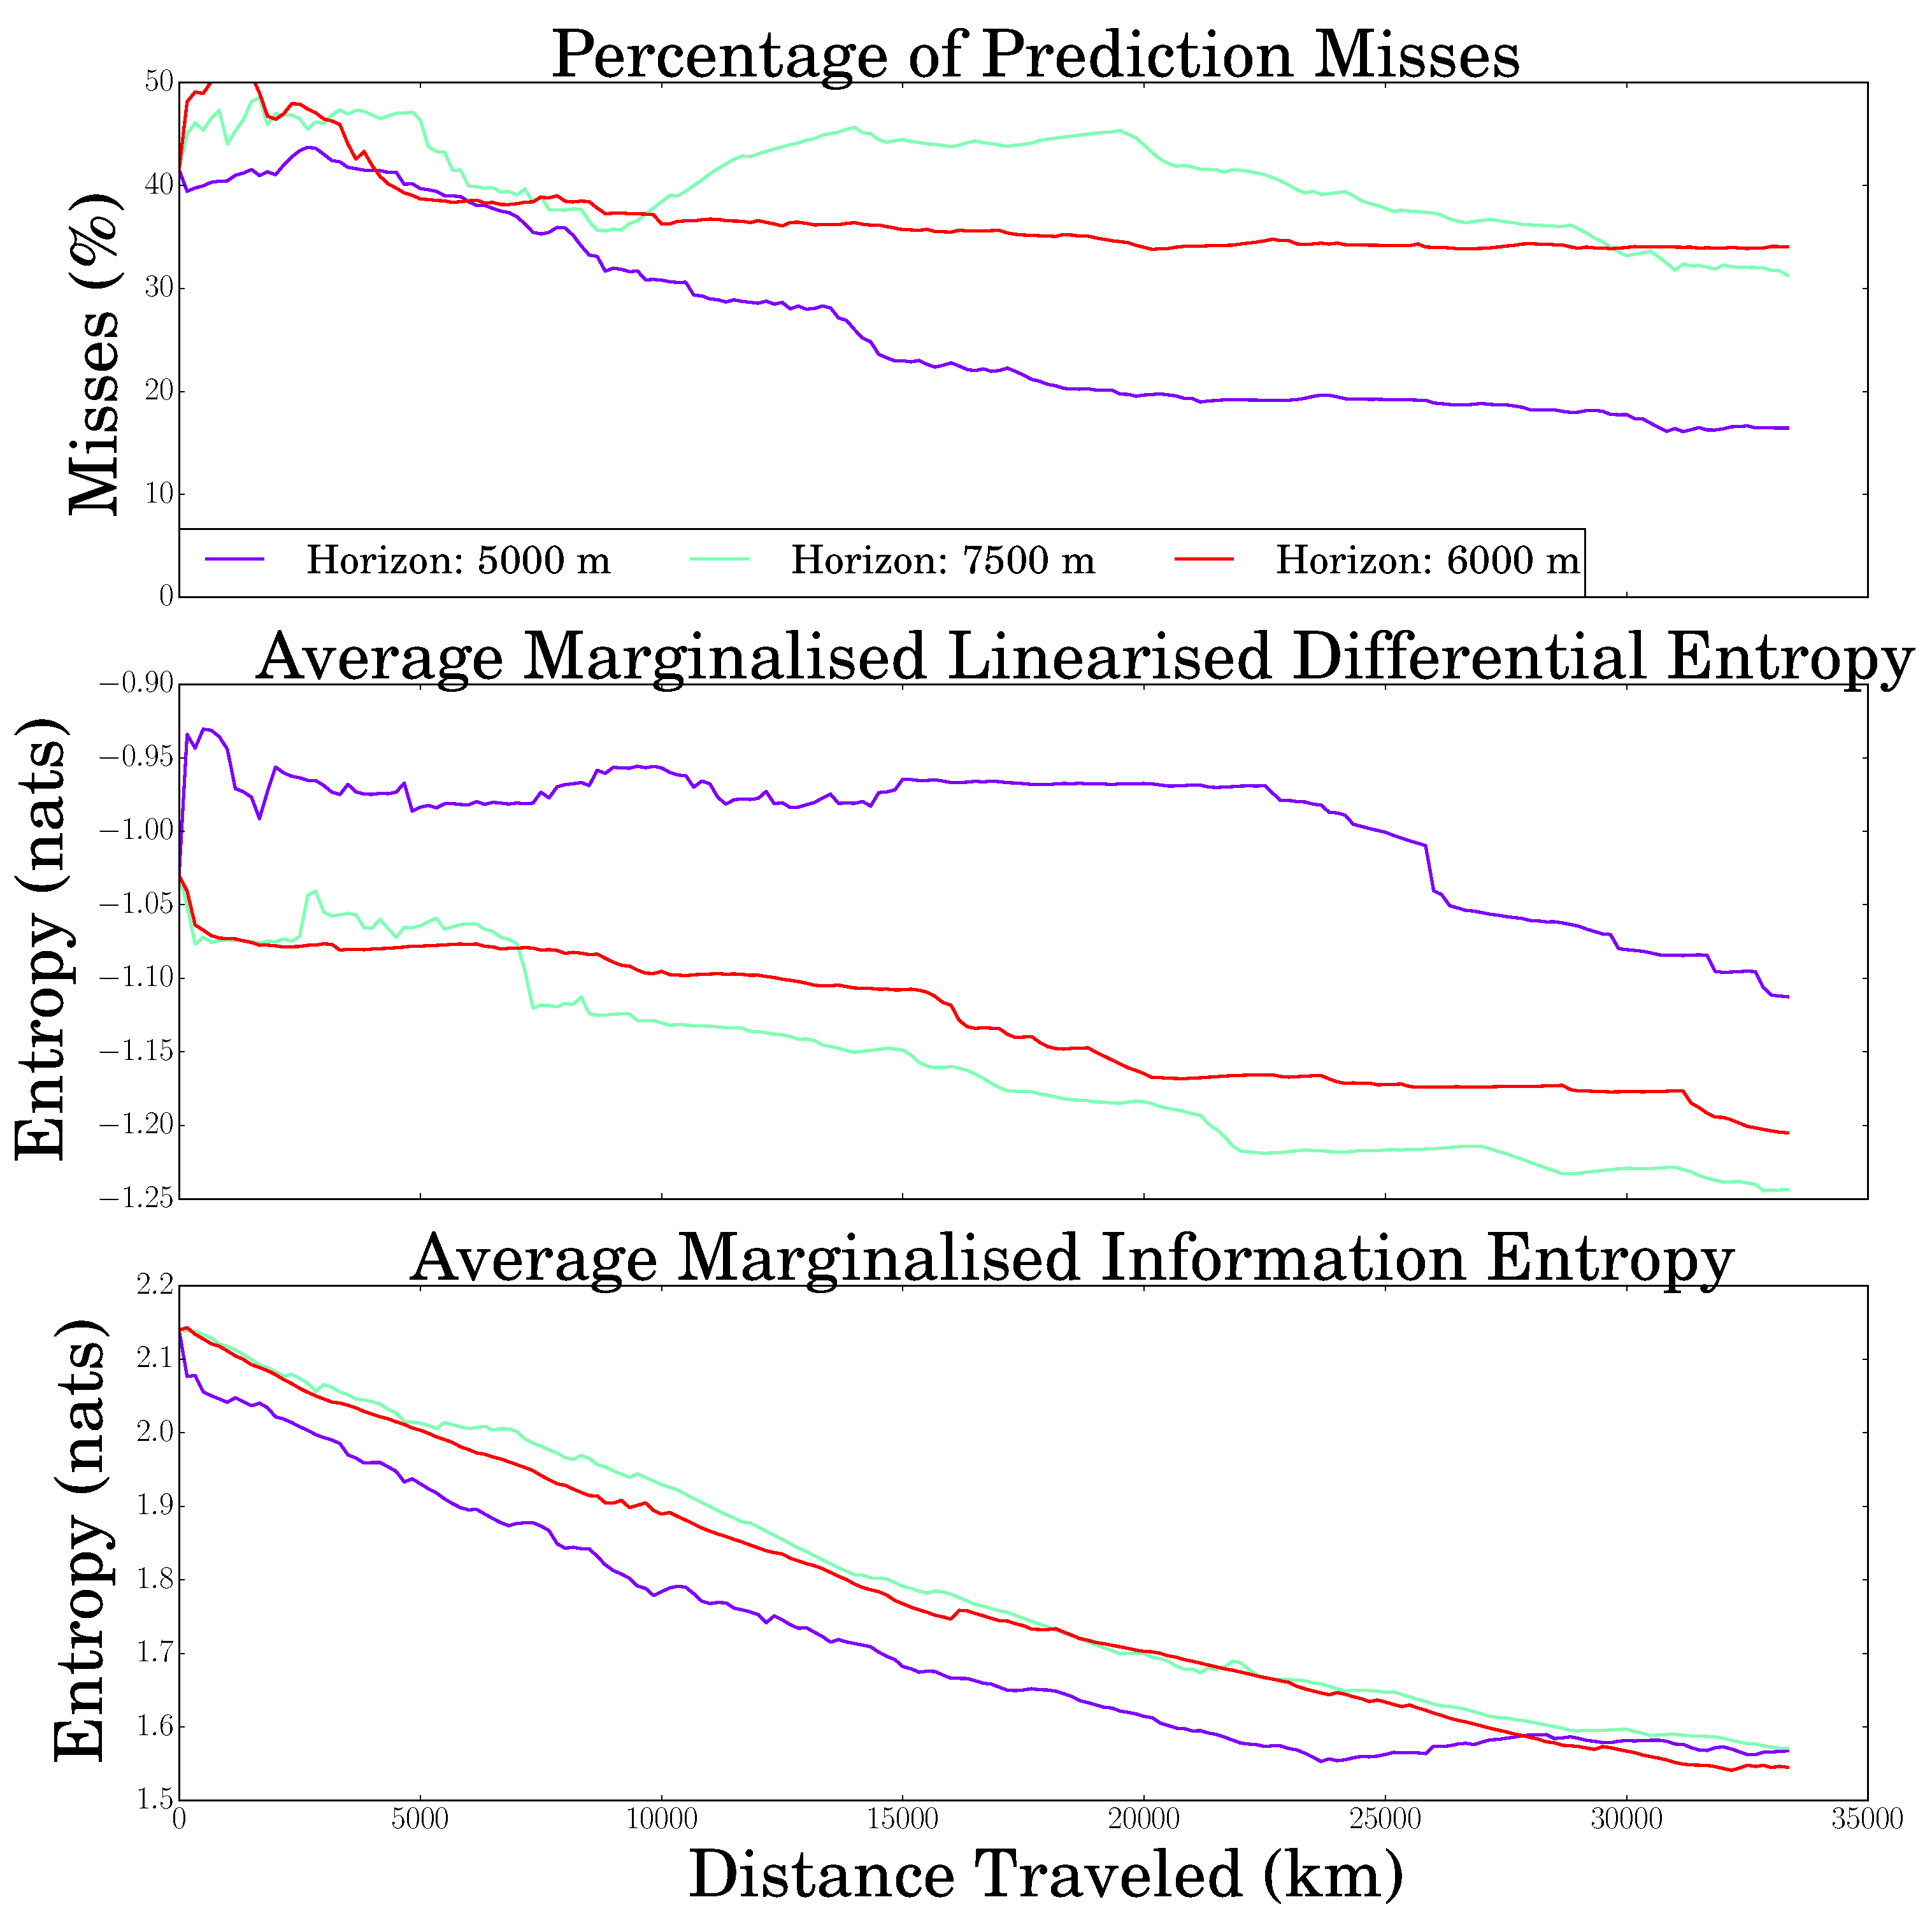
\includegraphics[width=0.48\linewidth]{Figures/compare_horizons.eps}}
			\caption{Variance across initial starting point and receding horizon lengths}
			\label{Figure:VarianceSimulation}
			\end{figure}	
				
			Figure \ref{Figure:VarianceSimulation} demonstrates the stability and consistency of the LMDE acquisition approach under varying horizon lengths and starting locations for the case of Scott Reef. 
			
	\section{Serial Mission Planning for Seafloor Exploration}
	\label{Appendix:SeafloorExplorationTimeLapse:Serial}
	
			\begin{figure}[!htbp]
			\centering
			  \subfigure[Journey: 1\%]{\label{Figure:SerialOptimalPaths:LMDE1} 
			  	\includegraphics[width = 0.31\linewidth]{Figures/informative_seafloor_exploration/serial_lmde/pred_propose1.eps}}
			  \subfigure[Journey: 5\%]{\label{Figure:SerialOptimalPaths:LMDE2} 
			  	\includegraphics[width = 0.31\linewidth]{Figures/informative_seafloor_exploration/serial_lmde/pred_propose10.eps}}
			  \subfigure[Journey: 25\%]{\label{Figure:SerialOptimalPaths:LMDE3} 
			  	\includegraphics[width = 0.31\linewidth]{Figures/informative_seafloor_exploration/serial_lmde/pred_propose50.eps}}
			  \subfigure[Journey: 50\%]{\label{Figure:SerialOptimalPaths:LMDE4} 
				\includegraphics[width = 0.31\linewidth]{Figures/informative_seafloor_exploration/serial_lmde/pred_propose100.eps}}
			  \subfigure[Journey: 75\%]{\label{Figure:SerialOptimalPaths:LMDE5} 
			  	\includegraphics[width = 0.31\linewidth]{Figures/informative_seafloor_exploration/serial_lmde/pred_propose150.eps}}
			  \subfigure[Journey: 100\%]{\label{Figure:SerialOptimalPaths:LMDE6} 
			  	\includegraphics[width = 0.31\linewidth]{Figures/informative_seafloor_exploration/serial_lmde/pred_propose199.eps}}
			\caption{Scott Reef: LMDE Acquisition}
			\label{Figure:SerialOptimalPaths:LMDE}
			\end{figure}

			Figures \ref{Figure:SerialOptimalPaths:LMDE} and \ref{Figure:SerialOptimalPaths:MCPIE} show snapshots of the exploration process for LMDE and MCPIE acquisition. 
			
			\begin{figure}[!htbp]
			\centering
			  \subfigure[Journey: 1\%]{\label{Figure:SerialOptimalPaths:MCPIE1} 
			  	\includegraphics[width = 0.31\linewidth]{Figures/informative_seafloor_exploration/serial_lmde/pred_propose1.eps}}
			  \subfigure[Journey: 5\%]{\label{Figure:SerialOptimalPaths:MCPIE2} 
			  	\includegraphics[width = 0.31\linewidth]{Figures/informative_seafloor_exploration/serial_mcpie/pred_propose10.eps}}
			  \subfigure[Journey: 25\%]{\label{Figure:SerialOptimalPaths:MCPIE3} 
			  	\includegraphics[width = 0.31\linewidth]{Figures/informative_seafloor_exploration/serial_mcpie/pred_propose50.eps}}
			  \subfigure[Journey: 50\%]{\label{Figure:SerialOptimalPaths:MCPIE4} 
				\includegraphics[width = 0.31\linewidth]{Figures/informative_seafloor_exploration/serial_mcpie/pred_propose100.eps}}
			  \subfigure[Journey: 75\%]{\label{Figure:SerialOptimalPaths:MCPIE5} 
			  	\includegraphics[width = 0.31\linewidth]{Figures/informative_seafloor_exploration/serial_mcpie/pred_propose150.eps}}
			  \subfigure[Journey: 100\%]{\label{Figure:SerialOptimalPaths:MCPIE6} 
			  	\includegraphics[width = 0.31\linewidth]{Figures/informative_seafloor_exploration/serial_mcpie/pred_propose199.eps}}
			\caption{Scott Reef: MCPIE Acquisition}
			\label{Figure:SerialOptimalPaths:MCPIE}
			\end{figure}
			

\addtocontents{toc}{\vspace{2em}}  % Add a gap in the Contents, for aesthetics
\backmatter

%% ----------------------------------------------------------------
\label{Bibliography}
\lhead{\emph{Bibliography}}  % Change the left side page header to "Bibliography"
\small
\bibliography{Bibliography}  % The references (bibliography) information are stored in the file named "Bibliography.bib"

\end{document}  % The End
%% ----------------------------------------------------------------